\documentclass[final,10pt,a4paper, DIV12,  twoside, onecolumn, openright, titlepage, headsepline, footsepline, bibliography=totoc,  toc=graduated, numbers=enddot, version=first]{scrbook} 
\usepackage[T1]{fontenc}
\usepackage[english,ngerman]{babel}
\usepackage[utf8]{inputenc}
\setkomafont{sectioning}{\rmfamily\bfseries\boldmath}
\setlength\parskip{1mm}
\setcounter{secnumdepth}{3}
% ngerman %use ngerman instead of english when compiling the pages with german abstract
\selectlanguage {english} 

\usepackage{subfigure}
\usepackage[dvips]{graphicx} \pdfcompresslevel=9
\widowpenalty=10000
\clubpenalty=10000

\usepackage{verbatim}
\usepackage{color}
\usepackage{longtable}
\usepackage{url}
\usepackage{rotating}
\usepackage{amsmath}
\usepackage{amsthm} %Ergänzung zu "amsmath"
\usepackage{amsfonts}
\usepackage{currvita}
\usepackage{datetime}
\usepackage{cite}
\usepackage{enumitem}

%when using algorithms use the following commands
\usepackage{algorithmic}
\usepackage{algorithm}
\usepackage{fancybox}
\numberwithin{algorithm}{subsection}  
\newcommand{\theHalgorithm}{\arabic{algorithm}}
\renewcommand{\algorithmicrequire}{\textbf{Input:}\text{ }}
\renewcommand{\algorithmicensure}{\textbf{Output:}\text{ }} 

%this is for PDF output formatting, please change the data accordingly
\definecolor{darkblue}{rgb}{0,0,.5}
\usepackage{t1enc,dfadobe}
\usepackage[pdftex, pagebackref=true,						colorlinks,linkcolor=darkblue,citecolor=darkblue,urlcolor=darkblue,
    bookmarks=false,
    pdfpagemode=UseNone,plainpages=false,
    pdftitle={Application of electric field sensing systems in smart environments},pdfpagelabels,
    pdfauthor={Andreas Braun},
    pdfsubject={Ph.D.\ Thesis, Technische Universit\"at Darmstadt},
    pdfkeywords={thesis keywords}]{hyperref}

%other stuff AB
\usepackage{booktabs}
\usepackage{tabularx}


\makeindex


% begin document
\begin{document}
%\title{Visual Analytics of Large Two-Dimensional Time-Series and Weighted Directed Graphs\\ with Applications in Finance and Economics}
\title{Application of electric field sensing systems in smart environments}%\\ with Applications in Finance and Economics}
\author{Andreas Braun}

%\date{Draft: \today}

\begin{titlepage}

\begin{center}

\vspace*{1.0cm}
%Huge
\huge {\bf Application of electric field sensing systems in smart environments}
\vfill

\begin{figure}[ht]
    \centering
        
\includegraphics[width=2cm]{athene.pdf}
\end{figure}

\vspace*{0.2cm}

\normalsize

dem Fachbereich Informatik \\
der Technischen Universität Darmstadt \\
vorzulegende \\

\vspace*{0.5cm}
\Large{\scshape DISSERTATION} \\
\vspace*{0.5cm}
\normalsize
zur Erlangung des akademischen Grades eines \\
Doktor-Ingenieurs (Dr.-Ing.) \\
von \\

\vspace*{0.3cm}

\Large { M.Sc. Andreas Braun\\}

{\normalsize geboren in Aschaffenburg, Deutschland } % in Klammern, da sonst zu dicht am Namen

\normalsize
\vspace*{0.2cm}
\vfill

\begin{tabular}{rl}
Referenten der Arbeit: & Prof.\ Dr.\ techn.\ Dieter~W.~Fellner \\ 
												& Technische Universität Darmstadt \\
												%\\
											& Prof.\ XXX \\
											& affiliation of Prof.\ XXX \\
												\\
Tag der Einreichung:  & \ddmmyyyydate \today \\
Tag der mündlichen Prüfung:  \\
\end{tabular}

\vfill

Darmstädter Dissertation \\
D 17

\vspace*{1.0cm}
\end{center}

\end{titlepage}


\newpage
\thispagestyle{empty}

\cleardoublepage

%Inhaltsverzeichnis soll römisch numeriert sein:


\cleardoublepage

\pagenumbering{roman}\setcounter{page}{1}
\chapter*{Erkl\"arung zur Dissertation}
\thispagestyle{empty}

Hiermit versichere ich die vorliegende Dissertation selbst\"andig nur mit den angegebenen Quellen
und Hilfsmitteln angefertigt zu haben. Alle Stellen, die aus Quellen entnommen wurden, sind als solche
kenntlich gemacht. Diese Arbeit hat in gleicher oder ähnlicher Form noch keiner Prüfungsbehörde
vorgelegen.

\vspace{2cm}

Darmstadt, den \ddmmyyyydate \today  \hspace{6cm} Andreas Braun


\cleardoublepage


\chapter*{Abstract}
\label{ch:abstracten}
Summarize the thesis in 1/2--1 page.
\selectlanguage{ngerman}
	\chapter*{Zusammenfassung}
\label{ch:abstractde}

Describe in German in 6--10 pages your thesis. This is compulsory for EN written thesis. Zusammenfassung auf Deutsch.
\selectlanguage{english}

\cleardoublepage

\tableofcontents

\cleardoublepage

\listoffigures

\cleardoublepage

\listoftables

\cleardoublepage

\pagenumbering{arabic}\setcounter{page}{1}

\chapter{Introduction}
Smart environments are comprised of numerous sensing and computing devices that are supporting a number of users in this environment on performing their tasks. Capacitive sensors are a technology that uses electric fields to sense the presence and certain properties of the human body. In this work I present an overview of this technology, how it can be applied in different relevant application scenarios and  based on various prototypes evaluate the particular benefits and limitations of this sensing technology. 
\section{Motivation}
In the last decade the way we interact with computing machines has changed in a profound fashion. Today more than one billion people operate a smartphone, enabling ubiquitous access to communication tools, processing power and information. The vision of ubiquitous computing as proposed by Mark Weiser in the early 90s is inching closer to reality \cite{Weiser1991}. The required technologies of \begin{quote}
"cheap, low-power computers that include equally convenient displays, a network that ties them all together, and software systems implementing ubiquitous applications" 
\end{quote}
are now existing in the form of smartphones and tablets that are connected to the internet, using high-speed connections such as LTE and web-based services such as Google Now, that combine numerous data sources to provide personalized services.

While the vision and underlying ideas remain similar other names have been used in research, including Pervasive Computing and Ambient Intelligence. The concept has been expanded to not only consider devices that can be directly manipulated, but include determining the situation and reacting based on it. This context-aware computing proposes 
\begin{quote}
"systems that examine and react to an individual's changing context. Such systems can promote and mediate people's interactions with devices, computers, and other people" \cite{schilit1994context} 
\end{quote}
Different forms of context can be distinguished, ranging from location and the actual system state, to different activities or even the current mood of the user. In order to acquire this context, the input-and-output based systems originally proposed by Weiser, are augmented by an ensemble of devices that are very small (dust), coordinate in massive numbers (clay) or are flexible, unobtrusive extensions to everyday objects (fabric) \cite{poslad2011ubiquitous}. This devices can be invisibly integrated into our everyday environment and provide sensing capabilities that can be used by sufficiently smart systems. Examples of these devices are microelectromechanical systems (MEMS) or bendable technology, such as OLED screens. The number of computation and sensing devices that we carry with us is growing continuously, yet we want the technology to further disappear, allowing us to focus on the application instead of the underlying technology. 

The famous science fiction author Arthur C. Clarke proposed three laws of prediction, the  third of which is 
\begin{quote}
"Any sufficiently advanced technology is indistinguishable from magic." \cite{clarke1962hazards} 
\end{quote}
Capacitive proximity sensing allows us to measure the influence of the human body (or conductive objects in general) on an electric field. While we would not call this technology magic, a peculiarity of electricity is that humans have no specific sensing organs, thus we generally remain unaware of their presence, unless the field strength is very high. Consequently, when interacting with capacitive sensors there is no awareness of what they are sensing unless it is specifically exposed to the user. The technology is well-understood and varieties have become ubiquitous in some areas, such as touch screens. However, there are numerous other applications for this technology, ranging from industrial fluid level and material detection, to presence detection for cars. A particularly interesting domain for this sensing technology are smart environments that provide services based on unobtrusively acquired information about persons currently acting in this environment. There are numerous sensing technologies that provide similar detection capabilities. Looking at the recognition of simple activities, such as standing, walking and lying, cameras and accelerometers can lead to the same result. Accordingly, in order to discuss the use a sensing technology within a specific domain, it is necessary to provide a benchmark that takes into account abstracted sensor properties and different application domains. In this work we will provide a generic benchmark model for different sensor technologies in smart environments and based on this discuss the use of capacitive proximity sensor technologies in this area. We will establish the most suited application domains and provide prototypes to evaluate different aspects.
\section{Research Challenges}
In the past there have been numerous great works that gave an overview of technologies and applications in smart environments. Cook et al. identified common technologies, frameworks and applications in this domain and give an overview of ongoing research. Poslad specified a more detailed taxonomoy of device classes, provides concepts for interaction between humans and environments and gives an overview of intelligent systems. A different category  of previous work details the different sensing technologies that are supporting various different applications and give an overview of limitations and benefits. However, so far there has been no work that provides a benchmark that maps different sensor characteristics to applications in smart environments. As it was stated by Cook et al.:
\begin{quote}
"Finally, a useful goal for the smart environment research community is to define evaluation mechanisms. While performance measures can be defined for each technology within the architecture hierarchy [...], performance measures for entire smart environments still need to be established. This can form the basis of comparative assessments and identify areas that need further investigation."
\end{quote}
In this work, we will contribute to this challenge and provide a benchmark based on methods previously presented by x. Using this benchmark we can identify application domains that are particularly suited for capacitive proximity sensors and provide a tool that allows researchers to select a suitable sensing technology for the given application.

The past few years have seen several emerging trends in computing, ranging from an increased connectivity of devices, driven by the Internet of Things, ubiquitous usage of mobile computing and sensing devices in the form of smartphones and tablets, and novel, natural interaction paradigms, that aim to provide human-machine interaction similar to interpersonal communication means. 

Driven by improved embedded technology, materials and an increase in computing power, it is possible to provide integrated systems based on capacitive proximity sensing that contribute novel aspects to several of these trends. In the last years we have created various prototypes in the identified application domains and applied state-of-the art sensor technology and novel algorithms. In this process we are able to provide numerous improvements to previously presented systems and enable new applications. Based on this it is possible to provide a thorough review of capacitive proximity sensing technology in the domain of smart environments.
\section{Contributions}
\begin{itemize}
\item Identification of application domains in smart environments
\item Develop benchmark model for mapping sensor features to smart environments
\end{itemize}

\section{Acknowledgments}
While many consider writing a PhD to be a mostly personal endeavor there are always various sources of discourse, collaboration, support and inspiration. 
So in no particular order there are various persons or groups of persons that deserve credit: 
\chapter{Related Work}
\section{Electric field sensing}
Any electric charge is applying an attracting or repelling force to other charged particles in space. This force has a distinct magnitude and direction for any point in space and thus creates an electric field. The presence of conductive objects is modifying the properties this field. Thus, in its most basic definition electric field sensing allows us to gather information about the field properties at a certain point in space. If we continuously monitor the field we are able to measure the disturbance and associate it to objects that are passing through, allowing to gather information about their specific properties. In this section we will give a brief overview of the development of electric field sensing technology, the physical background, different measuring modes and how to process data acquired by digital sensor devices.
\subsection{A brief history of capacitive proximity sensing}
\begin{figure}[h]
\centering
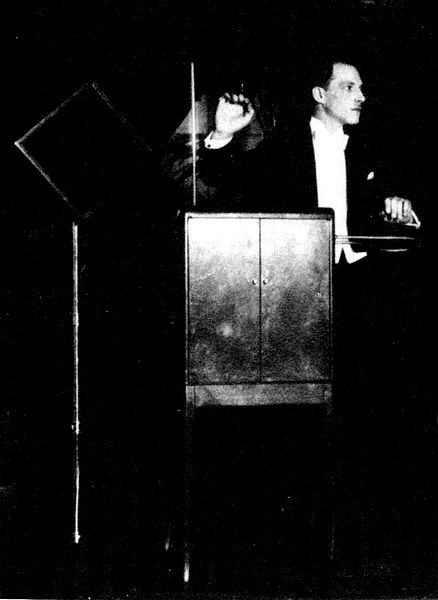
\includegraphics[width=0.4\textwidth]{images/leon_theremin.jpg}
\caption{Leon Theremin playing his epnoymous electronic musical instrument \cite{Glinsky2000}}
\label{fig:leon_theremin}
\end{figure}
In the last decades of the 19th and the beginning of the 20th century a considerable number of inventors and scientists performed research on the application of electric systems, sparking innovations such as electric lighting, electric motors, telegraphy and radio communication. Lev Sergeyevich Termen or Léon Theremin in the American naming was a Russian inventor most famous for designing the theremin. This early electronic musical instrument could be played without touch. One hand is controlling the pitch and the other the volume by changing the distance to an antenna. Initially designed as a motion detector, this device is transferring the influence of the human body on an oscillating electric field to an audible sound \cite{Glinsky2000}. 

Electric field imaging was a research focus at the MIT in the 1990s. A research group in the Media Lab division including Joseph A. Paradiso, Thomas G. Zimmerman, Joshua R. Smith designed various sensing devices and evaluated various applications in HCI \cite{Zimmerman1995}\cite{Smith1999a}.
\subsection{Physical properties}
A complete overview about the electrostatic principles of capacitive proximity sensing can be found in the book by Baxter \cite{Baxter1996}, chapters 2 and 6. We will give a very brief introduction to this topic in the following section.
\begin{figure}[h]
\centering
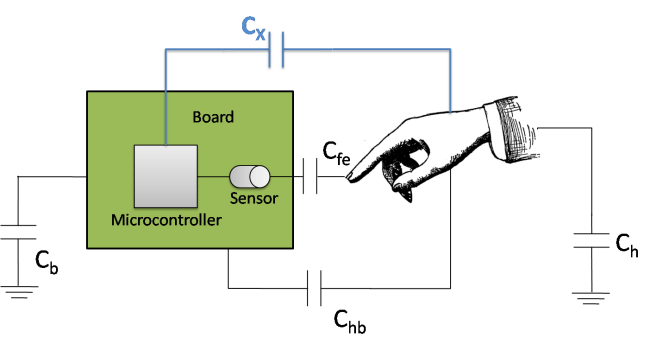
\includegraphics[width=0.4\textwidth]{images/cap_blackbox.png}
\caption{Black box setup of a capacitive proximity sensor}
\label{fig:cap_blackbox}
\end{figure}
The basic setup of a typically used sensor is shown in Figure \ref{fig:cap_blackbox}. The proximity capacitance \(C_{x}\) can be determined using a combination of serial and parallel circuits of capacitors, resulting in the following equation:
\begin{equation}
C_{x}=\left(\left(C_{hb}+\frac{C_{h}C_{b}}{C_{h}+C_{b}}\right)^{-1}\frac{1}{C_{fe}}\right)^{-1}
\end{equation}
Additionally there are parasitic capacitance components, i.e. disturbing capacitance values within the system. Sources are:
\begin{itemize}
\item Sensing electrode capacitance
\item Capacitance between sensing electrode and ground plane
\item Intercapacitance between neighboring traces on the board
\end{itemize}
The present parasitic capacitances \(C_{par}\) amount to values approximately between \(10pF\) and \(300pF\) and are therefore considerably larger than the value of the proximity capacitance \(Cx\), being between \(0.1pF\) and \(10pF\). The total capacitance sensed is the sum of parasitic and proximity components. 
\begin{equation}
C_{S}=C_{X}+C_{par}
\end{equation}

It is obvious that this parasitic capacitance is considerably higher than the capacitance induced by an approaching object. However, this parasitic capacitance is typically static and can therefore be calibrated in a way not affecting the measurement. 
\begin{figure}[h]
\centering
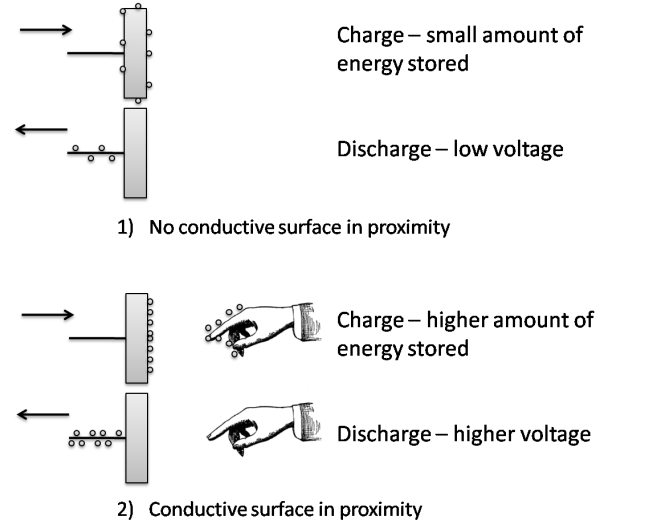
\includegraphics[width=0.4\textwidth]{images/cap_procedure.png}
\caption{Capacitive sensing procedure}
\label{fig:cap_procedure}
\end{figure} 
Now we will shortly discuss how we can estimate the capacitance of common objects that approach the sensor. Any object exhibits capacitance in respect to infinity. Surveying simple geometric shapes this capacitance is analytically determinable, e.g.:
\begin{equation}
C=8\epsilon_{0}r Disk
\end{equation}
\begin{equation}
C=4\pi\epsilon_{0}r	Sphere
\end{equation}

\(\epsilon_{0}\) is the vacuum permittivity and \(r\) the respective radius. This free space capacitance is increasing as soon as another object is approaching, caused by the capacitance of this second object, resulting in mutual capacitance. Looking at generic formulas, determining capacitance between parallel plates this behavior can be described analytically.
\begin{align}
C&=\frac{Q}{V} & C&=\epsilon_{0}\epsilon_{r}\frac{A}{d}
\end{align}
The capacitance is directly proportional to the plate area \(A\) and inversely proportional to the distance d between the plates, with \(\epsilon_{r}\) being the relative static permittivity of the dielectric between the plates. Sensor electronics are grounded with the body acting as ground itself. The sensor plate is continuously charged using a constant voltage \(V\). A higher capacitance allows the system to hold a larger charge. If the system is connected to the ground, the sensor capacitor is discharged through a resistor. The resulting voltage is depending on the available charge, shown in the equation above. Furthermore the required time to discharge the capacitor is increased. This process is symbolized in Figure \ref{fig:cap_procedure}.

\subsection{Proximity sensing versus touch sensing}
\begin{figure}[h]
\centering
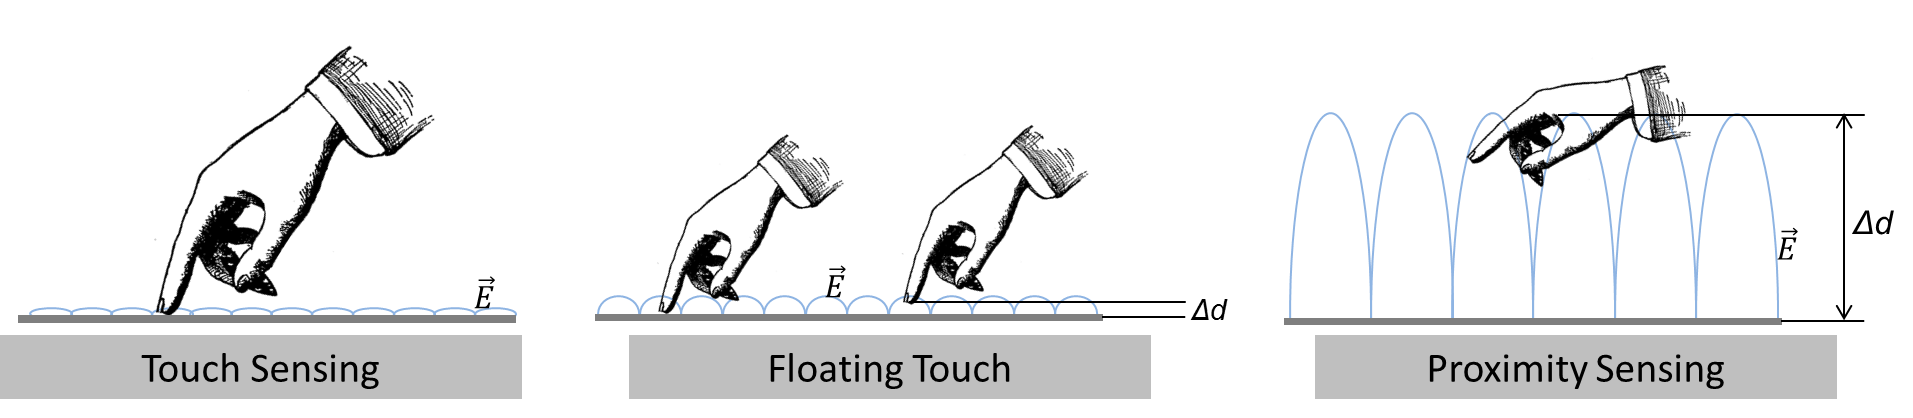
\includegraphics[width=1.0\textwidth]{images/cap_projected_sensing_methods.png}
\caption{Different projected capacitive sensing methods based on distance}
\label{fig:cap_proj_sensing_methods}
\end{figure} 
The most ubiquitous usage of capacitive sensing technology can be found in touch screens. As the trend went from pen-controlled mobile systems to finger controlled devices with the first iPhone in 2007, projected capacitance touch is the most prevalent technology for touch screens. It uses various layers of transparent electrodes or nanowires to detect the mutual capacitance as objects enter the detection area \cite{Barrett2010}. The commercially available devices have gained additional abilities over the last few years, leading to the development of “floating touch” systems that are able to track fingers in gloves or fingers that are hovering above the surface \cite{Cypress2012, Nokia2012}. Applications are the usage of mobile devices in cold outdoor temperatures or additional navigation fea-tures based on the hovering fingers. In consequence we can distinguish the three different projected capacitive sensing methods as shown in Figure \ref{fig:cap_proj_sensing_methods}:
\begin{itemize}
\item Touch sensing - densely distributed sensors are tuned to project a weak electric field in order to detect one or more objects touching the interactive surface. The sensors have to be close to the surface.
\item Floating touch - densely distributed high-sensitivity sensors are able to detect both touches and very near objects (\(<2cm\)) to enable usage using protective gear or additional navigation feature. The sensors have to be close to the surface.
\item Proximity sensing - sparsely distributed sensors create a stronger electric field that propagates into space in order to detect larger objects, such as hands, that are in proximity of the interactive surface. Achievable distances are up to 30 centimeters and the sensors may be applied below thick non-conductive material.
\end{itemize}
\subsection{Measuring modes}
\begin{figure} [h]
\centering
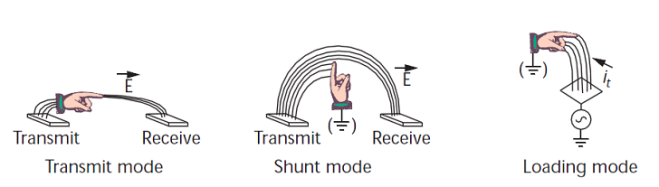
\includegraphics[width=0.6\textwidth]{images/cap_sensing_modes.png} 
\caption{Three measurement modes for capacitive proximity sensing \cite{Smith1996a}}
\label{fig:cap_sensing_modes}
\end{figure}
A classic work in the field of capacitive proximity sensing that will be referenced occasionally in this work is “Electric Field Imaging” by Joshua Smith \cite{Smith1999a}. One contribution was the introduction of different measurement modes in capacitive sensing, as shown in Figure \ref{fig:cap_sensing_modes}. 
Transmit mode is using a transmitting electrode that is coupled to a conductive object; in case of interaction applications typically the human body. The properties of an electric field generated with respect to a receiving electrode will therefore be dependent on the distance of this body, thus extending the achievable range.
Shunt mode similarly uses both a receiving and transmitting electrode generating a static field. However, there is no body coupled and any conductive object will ground the field, thus reducing the energy stored, which is measured. This setup is able to work with various transmitters on a single receiver, enabling a higher amount of virtual sensors using limited hardware. The third measurement mode is called loading mode. An oscillating field is induced on a single electrode measuring the capacitance relative to the environment. Any approaching grounded object results in an increased capacitance that is measured periodically.
\subsection{Materials and geometry}
Two major factors that have to be considered when designing an application based on capacitive sensors are the materials and geometry of the electrodes performing the measurements. The material of the electrode should be picked according to the desired application, i.e. if the interaction device has a flexible surface, conductive thread could be used, if it is solid and opaque, the application of solid metal electrodes is viable. Additionally there are other options for transparent materials. While we traditionally associate solid metals to antennas and electrodes this view can no longer be upheld. Transparent conductive layers have been in use for decades now, e.g. in car windows or solar technology. They typically rely on metal oxide layers, polymer layers or in recent years carbon nanotubes \cite{Moon2005}. The most common technology for usage in displays is projected capacitive touch that uses a multi-layer design of insulated ITO electrodes that are able to detect the movement of several objects close to the surface \cite{Barrett2010}. However, they are typically tuned to allow operation within a small distance of \(1cm\) or less. However, they are typically tuned to allow operation within a small distance of \(1cm\) or less. One recent work was evaluating different types of electrode materials in terms of their spatial resolution at different distances between object and electrode \cite{grosse2013opencapsense}, focusing on larger distance proximity measurements. They benchmarked both ITO and PEDOT:PSS. The first is a thin layer of indium-titanium-oxide, a highly conductive metal layer that possesses good optical properties. PEDOT:PSS is a conductive polymer that has a lower conductivity and slightly less appealing optical properties. In conclusion they evaluated that while copper has still the best properties, at least ITO can be considered a suitable alternative in applications that require optical clarity, as shown in the achievable spatial resolution given in Figure \ref{fig:cap_spatial_resolution}. 
\begin{figure} [h]
\centering
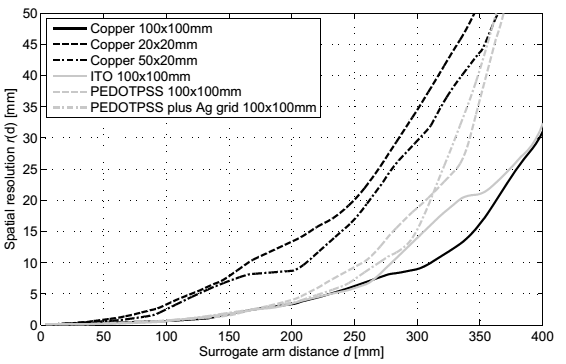
\includegraphics[width=0.6\textwidth]{images/cap_spatial_resolution.png} 
\caption{Spatial resolution of different materials at various distances \cite{grosse2013opencapsense}}
\label{fig:cap_spatial_resolution}
\end{figure}
The most common technology for usage in displays is projected capacitive touch that uses a multi-layer design of insulated ITO electrodes that are able to detect the movement of several objects close to the surface \cite{Barrett2010}. However, they are typically tuned to allow operation within a small distance of 1cm or less. 
Another area that is strongly influenced by the intended application is the geometry, whereas the electrode is considered the part of the electronics directly attached to the measurement circuit. This may range from simple straight wires or plate electrodes to complex optimized multidimensional structures specifically designed for a single task. Even though it is aimed at touch or near-proximity sensing we will give a short overview of  multi-layer designs for touch screens that have been reviewed by Barrett and Omote \cite{BarrettScreen}. They are designed to measure mutual capacitance, i.e. the resulting capacitive properties between a sending and a receiving electrode that are intersecting. If a sensible excitation and measuring process is used, multiple nearby objects may be reliably detected. 
\begin{figure} [h]
\centering
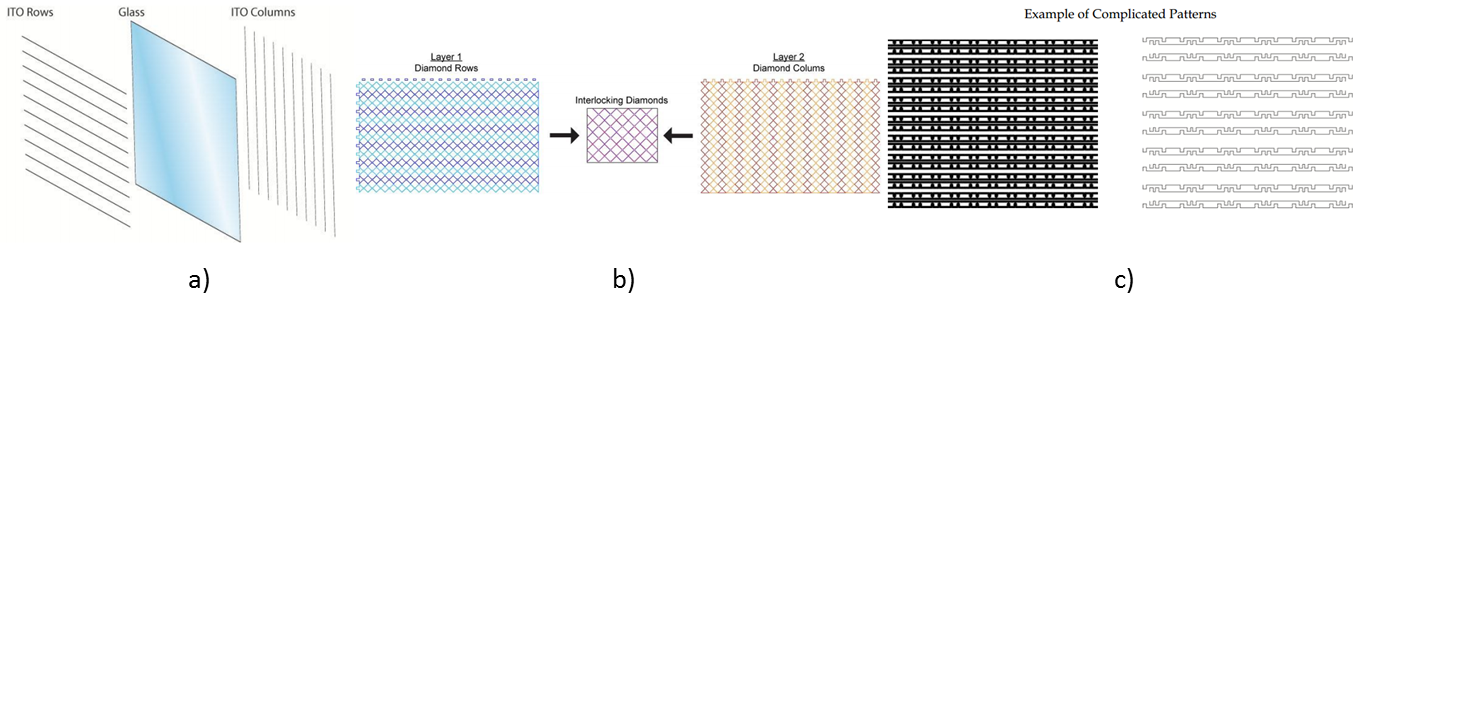
\includegraphics[width=0.8\textwidth]{images/ito_multilayer.png} 
\caption{Examples of multilayer layouts for touch screens - grid (a), interlocking diamonds (b) and  trademarked complex patterns (c) \cite{BarrettScreen}}
\label{fig:ito_multilayer}
\end{figure}
A simple example is two layers of perpendicular straight line electrodes - used by the first iPhone (Figure \ref{fig:ito_multilayer} - a). Another example uses an interlocking diamond shape \cite{Dietz2001a} to create a good spatial coverage (Figure \ref{fig:ito_multilayer} - b). Finally, there are numerous other complex patterns that are often trademarked by the companies that have developed the respective controller. One example is given in (Figure \ref{fig:ito_multilayer} - c). 

Capacitive proximity sensing applications are typically less concerned about intricate designs, but instead use varying electrode sizes and placement over a larger area. As previously mentioned the purpose of capacitive proximity sensing is the detection of objects and their properties. There are numerous factors that can influence the geometrical layout, but they can be abstracted into the following categories:
\begin{itemize}
\item	Number of objects
\item	Object size
\item	Desired spatial resolution
\end{itemize}
Going back to our example of touch screens, we have small objects, a higher number of those (usually up to 10) and require a high spatial resolution to select small items on the screen. The result is a fine multilayer grid, using mutual capacitance to simplify multi-object recognition, fine electrode spacing to achieve a high spatial resolution and thin or transparent electrodes to guarantee good optical properties. A similar rationale can be applied to other applications. If we take the smart couch by Große-Puppendahl et al. the aim is to detect the presence and posture of one or more persons on a couch \cite{Couch2011}. This necessitates detecting large body parts such as head, torso or limbs. There is no fine-grained spatial resolution required, allowing a reduction the number of sensors and it was assumed that a maximum of two persons are on the couch. Furthermore the electrodes are placed below the upholstery, thus requiring a reasonable detection distance. 
\begin{figure} [h]
\centering
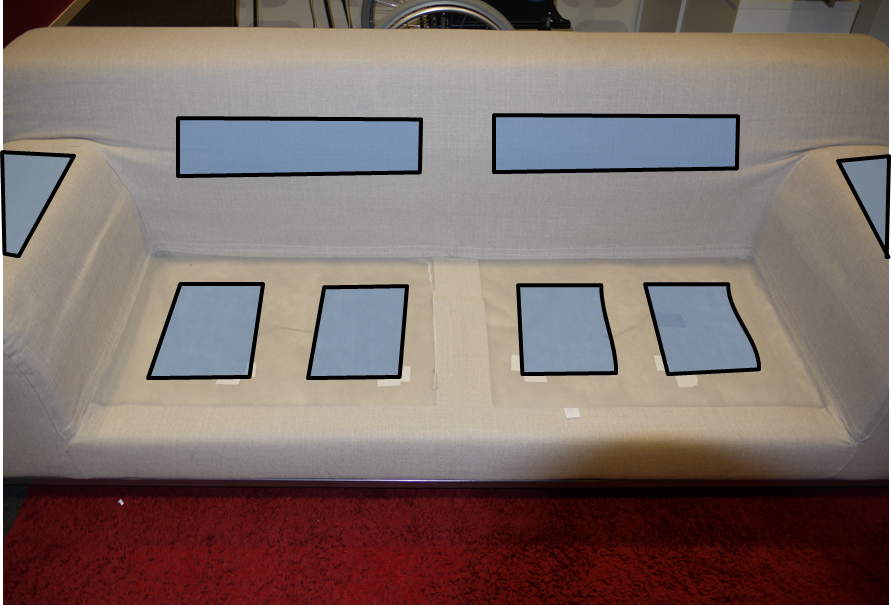
\includegraphics[width=0.7\textwidth]{images/couch_electrodes.png} 
\caption{Electrode placement below upholstery \cite{Couch2011}}
\label{fig:couch_electrodes}
\end{figure}
The resulting electrode placement can be seen in Figure \ref{fig:couch_electrodes}. The layout was designed under the additional constriction of using a single sensor kit, supporting up to eight electrodes. Regarding placement it is most important to distinguish two persons and different sitting positions, thus four electrodes are placed below the sitting area. In the back there are two electrodes spread over the entire width to determine the presence of the upper body close to the backrest. The electrodes in the armrests determine a head and are primarily suitable for detecting lying positions. In consequence this setup is suitable for detecting multiple sitting persons, infer information about their sitting position and recognize lying persons. Regarding those postures it showed good results in the prototype's evaluation \cite{Couch2011}.
 
A third and final example for the rationale of electrode placement is the TileTrack system by Valtonen et al, a capacitive person tracking system using floor tiles \cite{Valtonen2009a}. It is a transmit mode system that has the transmitting electrodes placed below the floor tiles and the receiving electrodes are placed in the walls of the area. The main goal of the system is the tracking of persons on the surface. Thus the floor area should be mostly covered by electrodes to establish a good transmission link to the bodies. The receiving electrodes should be able to pick up all signals generated by the body. Valtonen et al. picked wire or plate electrodes that went from floor level to a height of 190cm that covers most typical body sizes. While the system has some shortcomings with regard to applicability in larger rooms, the design rationale is appropriate for narrow rooms or when only movement close to walls has to be detected and had a reasonable precision in their evaluation.
Looking at the above examples it becomes apparent that the proper selection of materials and geometry is highly depending of the desired application. In consequence it is difficult to give generic guidelines independent of the application. After reviewing the different application domains in the next section we will revisit this topic in section 5.4.

\subsection{Data processing}
\begin{figure}[h]
\centering
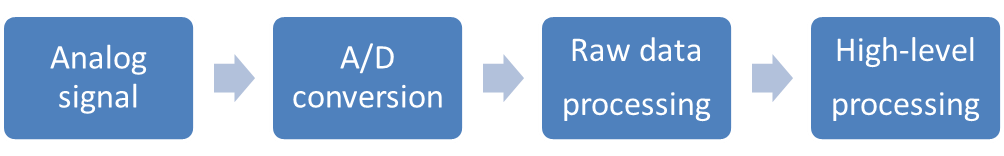
\includegraphics[width=0.4\textwidth]{images/proc_pipe}
\caption{Abstracted sensor data processing pipeline}
\label{fig:rel_proc_pipe}
\end{figure} 
%Figure 10 Abstracted sensor data processing pipeline
In order to acquire usable data from any digital sensor an analog signal has to be acquired and processed. A simplified typical processing pipeline for this is shown in Figure \ref{fig:rel_proc_pipe}. This basic structure is also applicable to the processing of capacitive proximity sensor data. The analog signal is the capacitance of an electric circuit that can be digitized using different methods, e.g. by using the quantized discharge time of the circuit. In the following section some typical steps of raw data processing and high-level processing for capacitive proximity sensors are presented and discussed. 
\subsubsection{Raw data processing}
Raw data processing of capacitive proximity sensor data is primarily intended to compensate for sensor noise and environmental influences. Noise is an inherent property of any measurement system and describes random unwanted data that is added to a signal. Environmental parameters can have strong influence on the signal of a capacitive sensor system. These effecting factors include temperature, humidity, composition of the air, or grounded objects in close proximity. There are numerous additional preprocessing steps that can be taken, such as different multiplexing methods that may be required in some hardware settings, or signal quantization that reduces the outgoing data to a distinct set of values in order to simplify post processing of different applications. These will not be further discussed in the scope of this work.
\paragraph{Noise Reduction}
In order to deal with noise, some sort of filtering is typically applied. Filtering describes a set of methods that attenuate the parts of a signal that are relevant in a given application. In capacitive proximity sensing we are dealing mostly with high-frequency noise that is added to the signal. Therefore, low-pass filtering can be used to deal with this influence. The most typical examples are average filters that take various samples and calculate an average value, and median filters that are sorting a set of samples and select the median element. Each of those filters has a plethora of potential adaptations that are not too specific to discuss in this limited space. Some adaptations are discussed in the specific prototype sections.
\begin{table}[htbp]
  \centering
  \caption{Baseline calibrations terms and methods}
    \begin{tabular}{lp{6cm}p{5cm}}
    \toprule
    \textbf{Name} & \textbf{Description} & \textbf{Application} \\
    \midrule
    \textbf{Initial calibration} & First set-up of baseline at system start, e.g. by taking the average over various samples & Required for any application \\
    \textbf{Static baseline} & Baseline that does not change at run-time & For static environments \\
    \textbf{Dynamic baseline} & Baseline that changes over time & For non-static environments \\
    \textbf{Drift } & Change of system response to environmental factors at run-time & - \\
    \textbf{Drift compensation} & Methods to account for occurring drift, by changing the baseline value & Non-static applications \\
    \textbf{Recalibration} & Change of the baseline value at a specific point in time given a set of rules & Non-static applications \\
    \bottomrule
    \end{tabular}%
  \label{tab:rel_baseline}%
\end{table}%


%Table 1 Baseline calibrations terms and methods
%Name	Description	Application
%Initial calibration	First set-up of baseline at system start, e.g. by taking the average over various samples	Required for any application 
%Static baseline	Baseline that does not change at run-time	For static environments
%Dynamic baseline	Baseline that changes over time	For non-static environments
%Drift 	Change of system response to environmental factors at run-time	-
%Drift compensation	Methods to account for occurring drift, by changing the baseline value	Non-static applications
%Recalibration	Change of the baseline value at a specific point in time given a set of rules	Non-static applications

\paragraph{Baseline Calibration}
A very important aspect of capacitive raw data processing is signal calibration. The generated electric field is subject to changes over time, if either intrinsic parameters change or the environment is modified. Some specific examples include the electronic components heating up, the environmental temperature changing, or objects being moved in and out of detection range. Therefore it is essential to have a well-calibrated and adaptive baseline; that is the sensor signal generated in the environment without the presence of any object that we want to detect. Again, there are numerous methods to adapt and configure the baseline. We have collected a few common terms and methods and give some pointers regarding their application. The results are shown in Table \ref{tab:rel_baseline}. 
\begin{figure}[h]
\centering
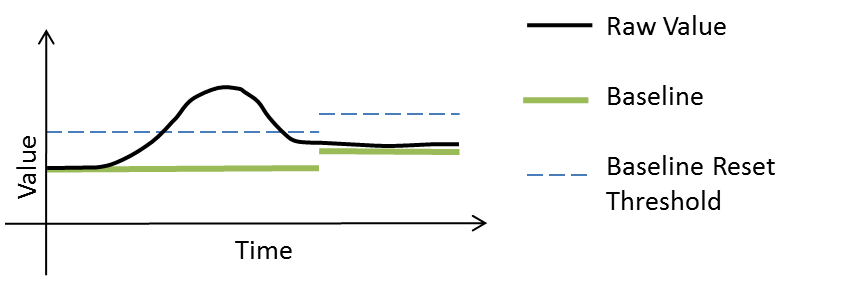
\includegraphics[width=0.5\textwidth]{images/baseline_reset}
\caption{Example of baseline reset using a threshold rule}
\label{fig:rel_base_reset}
\end{figure} 
%Figure 11 Example of baseline reset using a threshold rule
If a dynamic baseline is used, a set of rules will have to be defined that determines at which points in time the baseline has to be recalibrated, what specific methods should be used and the set of parameters that control the methods. One simple example is to define a threshold level that triggers a baseline calibration, as shown in Figure \ref{fig:rel_base_reset}. The raw signal is above the threshold, indicating the presence of a detectable object. Afterwards, it falls back down below the threshold, yet stays for a certain time above the baseline. This triggers a reset of the baseline after a certain amount of time.
\subsubsection{High-level processing}
High-level processing assumes that we already have calibrated (and possibly normalized) sensor values that are used in further steps. The goal of any capacitive sensing application is the acquisition of information about a detectable object, e.g. its current position, the material used or the shape. In order to get this information we need to use knowledge about the object and intrinsic properties of the sensor system. In this section we will discuss methods to combine data from various sensors using the system properties, how to track the position of an object using different methods and how to recognize specific features. An overview of the methods in abridged form is given in Table \ref{tab:rel_highlevel}. 
\begin{table}[htbp]
  \centering
  \caption{Overview of high-level processing methods for capacitive proximity sensors}
    \begin{tabular}{lp{5cm}}
    \toprule
    \textbf{Name} & \textbf{Description} \\
    \midrule
    \textbf{Sensor data fusion} & Combining sensor data into a shared representational format \\
    \textbf{Uniform fusion} & Sensor data fusion that combines all data into a single common format \\
    \textbf{Heterogeneous fusion} & Sensor data fusion that combines groups of data to serve multiple purposes \\
    \textbf{Object tracking } & Continuous identification of an object within the systems range \\
    \textbf{Single object tracking} & Methods to realize object tracking for a single detectable object \\
    \textbf{Multiple object tracking} & Methods to realize object tracking for multiple objects \\
    \textbf{Feature recognition} & Identifying certain parameters of an object within the system range \\
    \bottomrule
    \end{tabular}%
  \label{tab:rel_highlevel}
\end{table}%

%Table 2 Overview of high-level processing methods for capacitive proximity sensors
%Name	Description
%Sensor data fusion	Combining sensor data into a shared representational format
%Uniform fusion	Sensor data fusion that combines all data into a single common format
%Heterogeneous fusion	Sensor data fusion that combines groups of data to serve multiple purposes
%Object tracking 	Continuous identification of an object within the systems range 
%Single object tracking	Methods to realize object tracking for a single detectable object
%Multiple object tracking	Methods to realize object tracking for multiple objects
%Feature recognition	Identifying certain parameters of an object within the system range

\paragraph{Sensor data fusion}
Sensor data fusion in its most general terms describes “the theory, techniques and tools which are used for combining sensor data, or data derived from sensory data, into a common representational format” \cite{mitchell2007introduction}. Using the combined information from various capacitive proximity sensors we are able to generate high-level information that exceeds the capabilities of a single sensor. We can distinguish uniform fusion that uses the information from all involved sensors in one common way or heterogeneous fusion that combines groups of involved sensors that serve multiple purposes, yet are attached to a single system. A simple example for the latter would be a single large electrode sensor that detects the presence of a hand from a farther distance and then a combination of various small electrodes that track single fingers. 
Sensor data fusion often requires taking into account some additional information we possess about the system. A classic example is the precision or bias of the sensor. Various methods, e.g. the class of Kalman filters, use weighted information from several sensor sources \cite{welch1995introduction}. If we know how that a certain sensor is only half as precise as another one working in collaborating, the weighting factors can be adapted accordingly. 

One of the most important additional information we use when fusing data of capacitive proximity sensors, is the geometric layout of the system. This describes position and size of all electrodes that are integrated. Using this information is crucial when trying to localize an object. A simple example would be applying a weighted average algorithm on a set of sensors. In order to determine object location relative to the plane a weighted average algorithm is used. The linear object location $\overline{x}$ is calculated using the sums over sensor positions $x_i$ and sensor values $v_i$ as weight:
\[\overline{x}=\frac{\sum^n_{i=1}{v_i x_i}}{\sum^n_{i=1}{v_i}}\]

Using similar methods we are able to determine the location of multiple objects or additional dimensions of the position.
However, it is possible to use other information in the fusion process as well. The electrode material may result in a different response and thus should be treated differently in a fused data representation and can be weighted. Another example is the shape of the electrode that may result in different responses. How to apply sensor data fusion is strongly depending on the application and the desired common representation that is most suitable for subsequent calculations.

\paragraph{Object tracking}
In the previous section about sensor data fusion we have shortly discussed a method to determine the linear position of a single object using a linear array of capacitive proximity sensor. This is a basic example of a group of methods associated to object tracking. In computer vision applications they can be defined as “the problem of estimating a trajectory of an object in an image plane as it moves around a scene” \cite{yilmaz2006object}. The analogy to capacitive applications is viable if we consider a 3D scene and a distinct interaction space instead of a scene. 
Capacitive proximity sensors allow the detection of conductive objects within their range. However, as this presence is determined indirectly using the influence on an electric field it is not possible to get a direct association between the actual distance between sensor and object and the resulting sensor value. The created electric field is only analytically descriptive for very specific, theoretic classes of objects \cite{Baxter1996}. Nonetheless, we are able to get a relative distance measurement. If we combine this proximity value using geometric information about the electrode location we can infer the relative position of an object in the sensing area. The weighted average method presented in the previous section is one option for relative positioning. Another method is trilateration, similar to many radio-based localization applications, that uses the known location of three or more points and the known distance to the position to be determined. In case of capacitive proximity sensing this position is determined relative to the electrodes as there is no absolute distance measurement. 
A more complex example for direct calculation was presented by Smith, who formulated the issue of detecting multiple objects as a forward problem and used numerical methods to estimate the position and orientation of two hands \cite{Smith1999a}.
\begin{figure}[h]
\centering
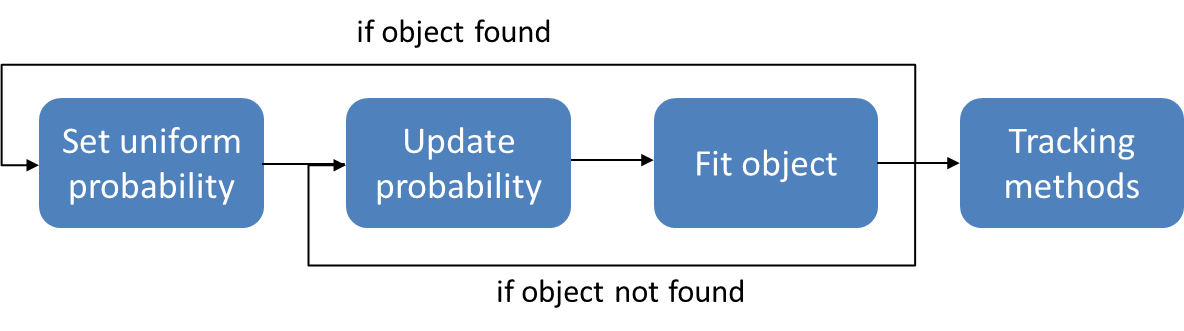
\includegraphics[width=0.5\textwidth]{images/prob_methods}
\caption{Generic pipeline of probability based methods of capacitive proximity sensing}
\label{fig:rel_prob_method}
\end{figure}
%Figure 12 Generic pipeline of probability based methods of capacitive proximity sensing
A second class of methods to track objects is not relying on direct geometrical calculations but instead formulates a numerical solution to a probability distribution. The initial assumption is that the probability of an object to be at a certain point in the detection area is uniform. The methods then follow a few basic steps, as shown in Figure \ref{fig:rel_prob_method}. At first the probability is updated based on the current sensor readings and a priori knowledge that we have about the system. Afterwards we try to fit the objects into the resulting probabilities. This step may or may not work, meaning that it may result in no object found. In the latter case the process will have to start at the beginning. If an object is found the probability update may use the current object location in the update algorithm, thus starting with a non-uniform probability distribution.
One example for probability-based object recognition using capacitive proximity sensors was presented by Grosse-Puppendahl et al. \cite{grosse2013swiss}. Using a model suggested by Smith the basic idea is using the assumption that an object may be present anywhere, remove regions where no objects can be present and then fit an object into the remaining space. This method additionally uses particle filters to track object locations over time. This also allows tracking multiple objects. 
Throughout the years various methods have been suggested for supporting multi-object tracking using capacitive sensors. Touch screens often use inversion of the sender signal to reliably detect the positions of multiple points; however, this method can’t be used in proximity applications \cite{wilson2007}. Some of the previously presented methods support the tracking of two or more objects. There are still various limitations, particularly if not only the object location but also various other features such as rotation should be tracked. This is still an area of ongoing research, leading to the next area of high-level processing - feature recognition.
\begin{table}[htbp]
  \centering
  \caption{Feature recognition methods}
    \begin{tabular}{lp{7cm}}
    \toprule
    \textbf{Name} & \textbf{Description} \\
    \midrule
    \textbf{Data-driven  methods} & Directly associate input data to output features using various methods, e.g. machine learning and training data \\
    \textbf{Model-driven methods} & Input data is manipulating a pre-defined model of the system that is latter mapped to the output \\
    \textbf{Neural networks} & Computational models using a network of neuron-like objects that are often used in machine learning \\
    \textbf{Pattern recognition} & Methods that look for certain patterns in a set of input data \\
    \textbf{Semantic mapping} & Methods to realize object tracking for a single detectable object \\
    \bottomrule
    \end{tabular}%
  \label{tab:rel_feature}%
\end{table}%

%Table 3 Feature recognition methods
%Name	Description
%Data-driven  methods	Directly associate input data to output features using various methods, e.g. machine learning and training data
%Model-driven methods	Input data is manipulating a pre-defined model of the system that is latter mapped to the output
%Neural networks	Computational models using a network of neuron-like objects that are often used in machine learning
%Pattern recognition	Methods that look for certain patterns in a set of input data
%Semantic mapping	Methods to realize object tracking for a single detectable object

\paragraph{Feature recognition}
Feature recognition is primarily used as a term in image processing, traditionally in computer-aided design applications to recognize specific geometric properties of an object but also picture analysis, e.g. in facial recognition \cite{han2000manufacturing}\cite{belhumeur1997eigenfaces}. 
In the domain of capacitive proximity sensing, feature recognition can be defined as the acquisition of non-location information from any detectable object. An important feature in industrial applications is the material of an object \cite{Baxter1996}. With regards to recognizing additional features a system was presented by Wimmer et al. - Thracker \cite{Wimmer2006}, a prototype augmenting a regular monitor with capacitive proximity sensors. In addition to recognizing hand position the system is able to detect grasp gestures, which can be used to select items on the screen and perform pick and drop operations. Capacitive sensors can also be used to distinguish between persons and a children’s seat on the passenger side of a car \cite{george2009seat}. 
The methods to recognize the features can be divers, ranging from typical machine learning algorithms, to model-based approaches. An incomplete list is given in Table \ref{tab:rel_feature}. In order to keep this work contained we refrain from a deeper discussion at this point.


\section{Capacitive proximity sensing applications}
\label{ch:rel_capapps}
\begin{minipage}{\linewidth}
\centering
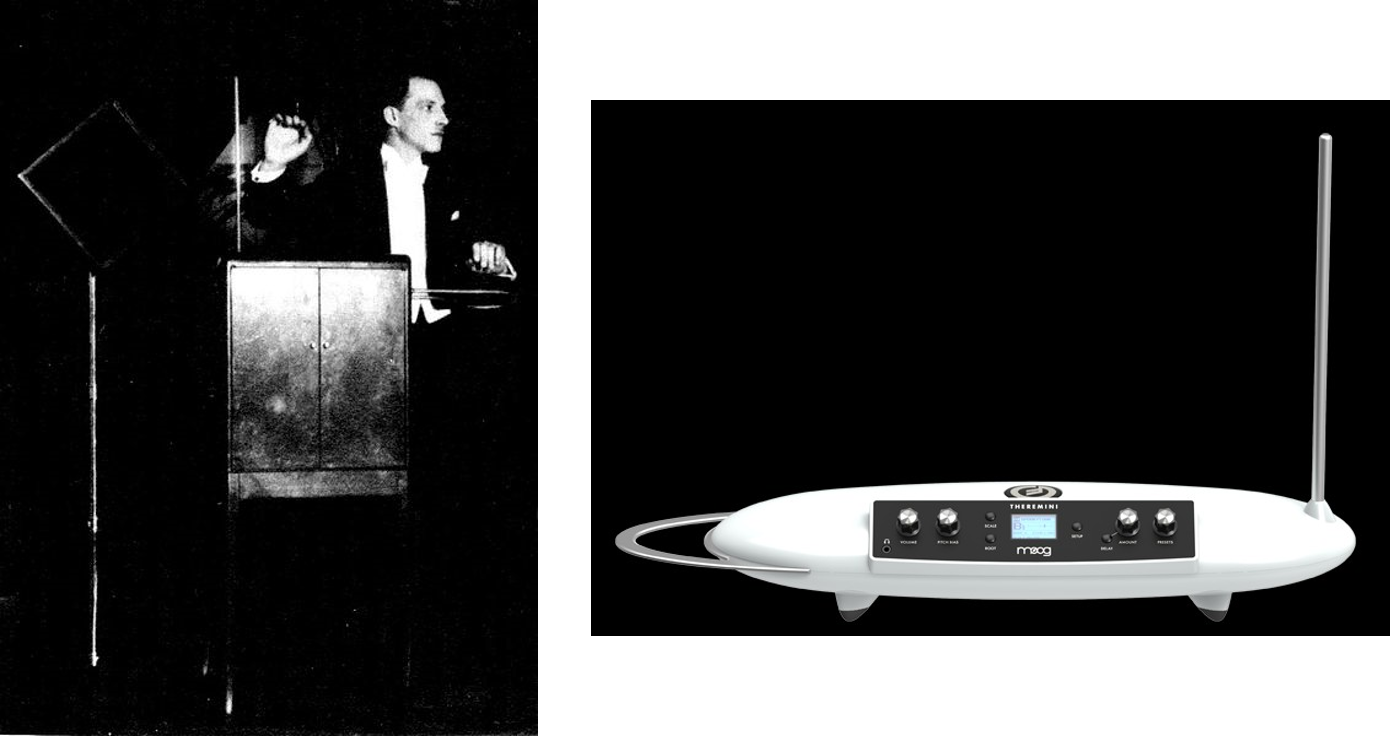
\includegraphics[width=0.9\textwidth]{images/theremins}
\captionof{figure}{\emph{Left:} Leon Theremin playing his epnoymous electronic musical instrument \cite{Glinsky2000}. \emph{Right:} The Theremini by Moog Music Inc., released in 2014 \cite{moog2014}}
\label{fig:theremins}
\end{minipage}
In the last decades of the 19th and the beginning of the 20th century a considerable number of inventors and scientists performed research on the application of electric systems, sparking innovations such as electric lighting, electric motors, telegraphy, and radio communication. Lev Sergeyevich Termen or Léon Theremin in the American naming was a Russian inventor most famous for designing the eponymous theremin. This early electronic musical instrument could be played without touch. One hand is controlling the pitch and the other the volume by changing the distance to an antenna. Initially designed as a motion detector, this device is transferring the influence of the human body on an oscillating electric field to an audible sound \cite{Glinsky2000}. Léon Theremin can be seen playing the instrument in Figure \ref{fig:theremins} on the left. This instrument is still in production to this day, with the electronic music instrument company Moog releasing a new variety that simplifies the sound production by fitting the distance to a sound on a specific musical scale \cite{moog2014}. The instrument is shown in Figure \ref{fig:theremins} on the right.

Electric field imaging was a research focus at the MIT in the 1990s. A research group in the Media Lab division including Joseph A. Paradiso, Thomas G. Zimmerman, Joshua R. Smith designed various sensing devices and evaluated various applications in in the domains of human computer interaction, smart appliances and reactive systems. They drew inspiration from biological precedents - various species of fish, such as Gymnotoidei can sense their surroundings using electric fields \cite{smith1999thesis}. The changing currents created by objects with a different dielectric constant from water can be registered and thus used to avoid obstacles, even if no light source is available. Accordingly, the group named some of their prototypes after this biological precedent, including the LazyFish and School of Fish \cite{smith1999thesis}. The research group created various different applications in the domains of human computer interaction, smart appliances and reactive systems.

\begin{minipage}{\linewidth}
\centering
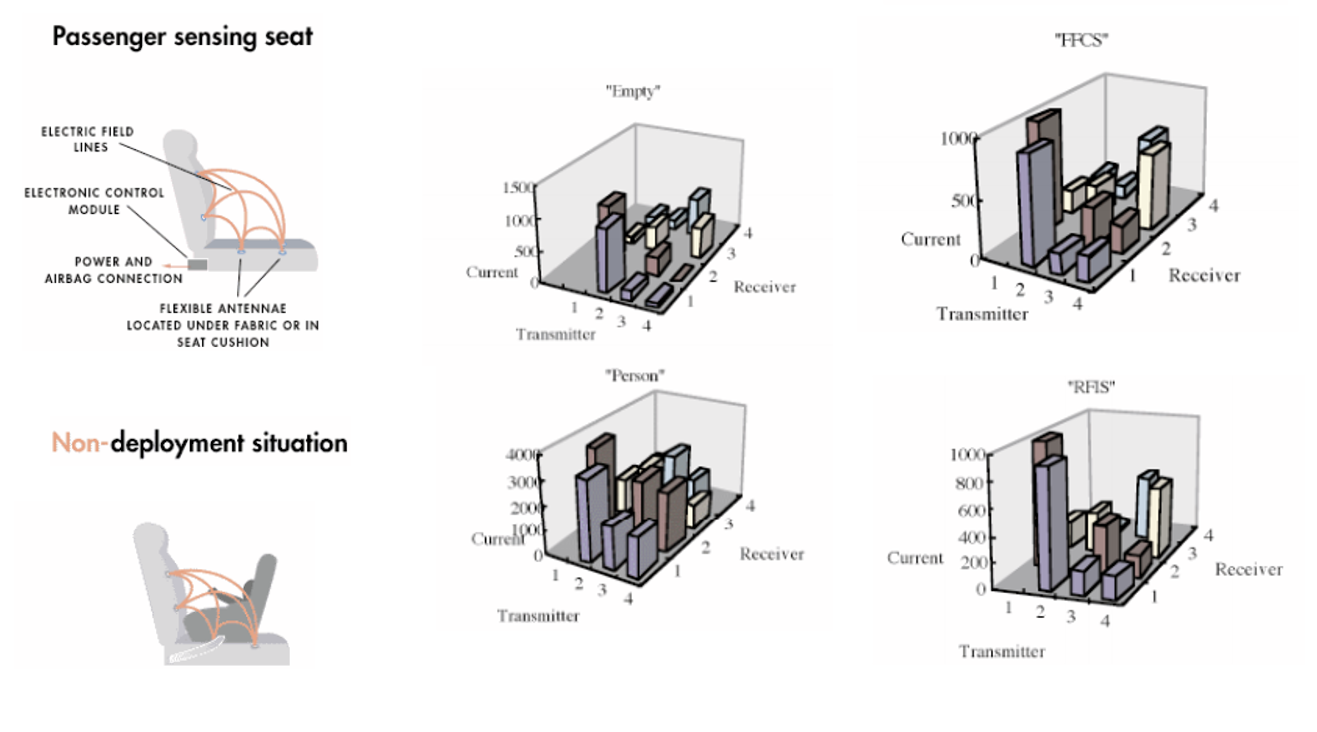
\includegraphics[width=0.9\textwidth]{images/nec_passenger_seat}
\captionof{figure}{\emph{Left:} Concept view of passenger seat set to deploy or not deploy airbag. \emph{Center:} Sensor readings for empty seat and adult person. \emph{Right:} Sensor readings for front-facing child seat (FFCS) and rear-facing child seat (RFCS). \cite{smith1999thesis}}
\label{fig:nec_passenger_seat}
\end{minipage}

In collaboration with NEC a smart passenger seat was created that incorporated capacitive sensors operating in shunt mode to detect if an infant seat is currently present on the passenger seat of car \cite{grosse2012enhancing}. The underlying challenge is that an airbag deployment should be prevented in such cases to prevent potential injuries to the infant. The seat is able to distinguish four different states, “No passenger”, “adult passenger”, “front-facing infant seat” and “rear-facing infant seat”. It uses four sending and four receiving electrodes and classifies the situation according to the current readings - the concept and readings of the sensors in the different situations are shown in Figure \ref{fig:nec_passenger_seat}.

\begin{minipage}{\linewidth}
\centering
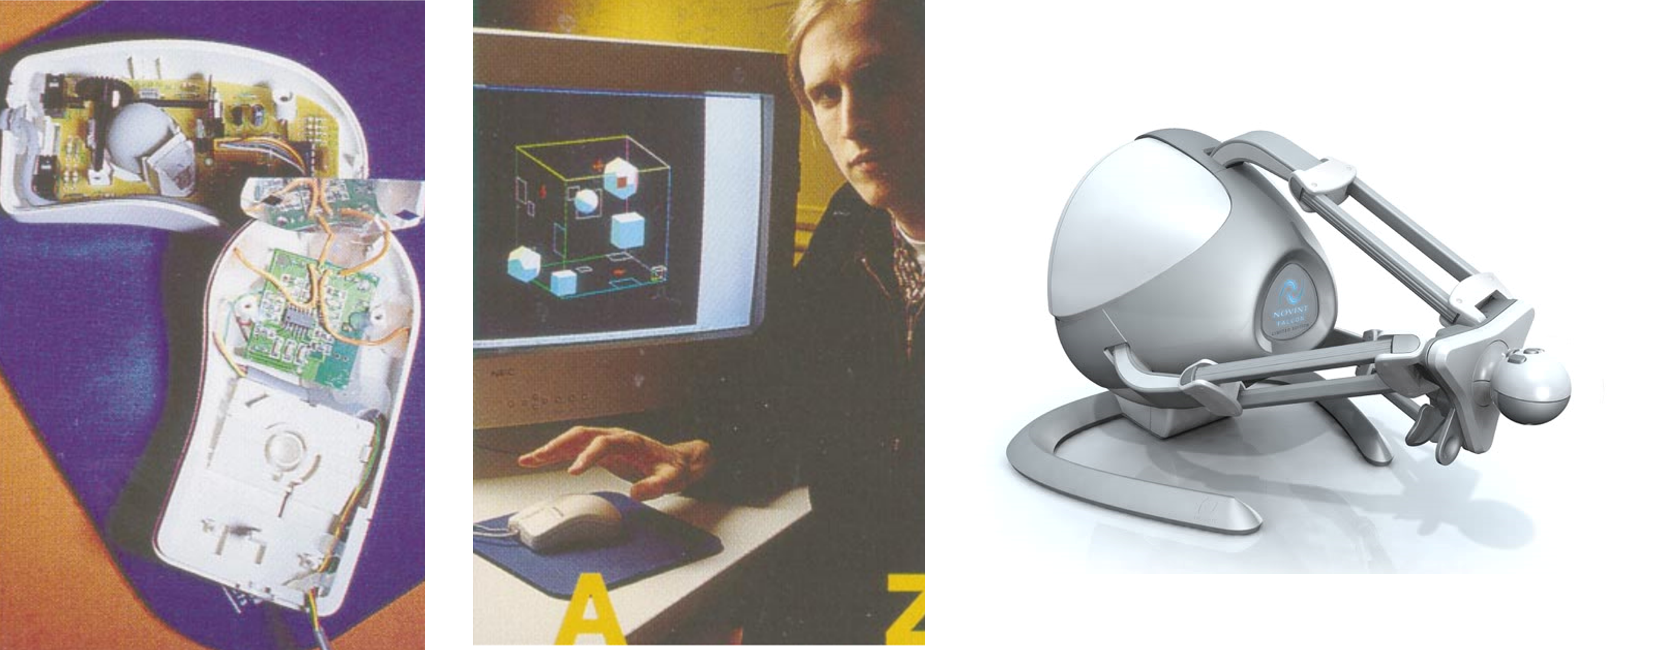
\includegraphics[width=0.9\textwidth]{images/lazmouse}
\captionof{figure}{\emph{Left:} LaZmouse innards \emph{Center:} Joshua R. Smith using LaZmouse \cite{smith1999thesis} \emph{Right:} Novint Falcon 3D input device \cite{novint2014}}
\label{fig:lazmouse}
\end{minipage}

Another prototype is the LaZmouse that extends a regular mouse with shunt mode capacitive sensors, having one transmitting and two receiving electrodes, to measure the proximity between the heel of the hand from the mouse surface, thus allowing the fingers to remain in the common position and the mouse to be moved around \cite{smith1999thesis}. Effectively this creates an input device with three degrees-of-freedom, enabling to perform interactions with a mouse that would usually require a more specialized 3D input device, such as the Novint Falcon that tracks the movement of the moved interaction sphere in three dimensions \cite{novint2014}. Figure \ref{fig:lazmouse} shows on the left, the electronics inside the mouse, the inventor using the device and a graphical representation, and on the right the Novint Falcon.

In another work Paradiso et al. presented numerous applications for capacitive proximity sensors, including smart furniture devices \cite{ Zimmerman1995}. They propose a smart table, comprised of a single transmitter electrode and two receivers that is able to track the position of a hand in two dimensions, a chosen dimension on the table and height. It may be used as gesture input device or to augment video desk applications. They also installed the system in a room, whereas the floor is a single electrode and there are four receivers located on the walls. This allows to infer the location of a person, based on relative signal strength. An additional system in this work is the smart chair, using a single transmitter in the seat and four receivers in the armrests and headrest. It allows to navigate through various audio channels based on head and arm movements \cite{ schmandt1995audiostreamer}.

\begin{minipage}{\linewidth}
\centering
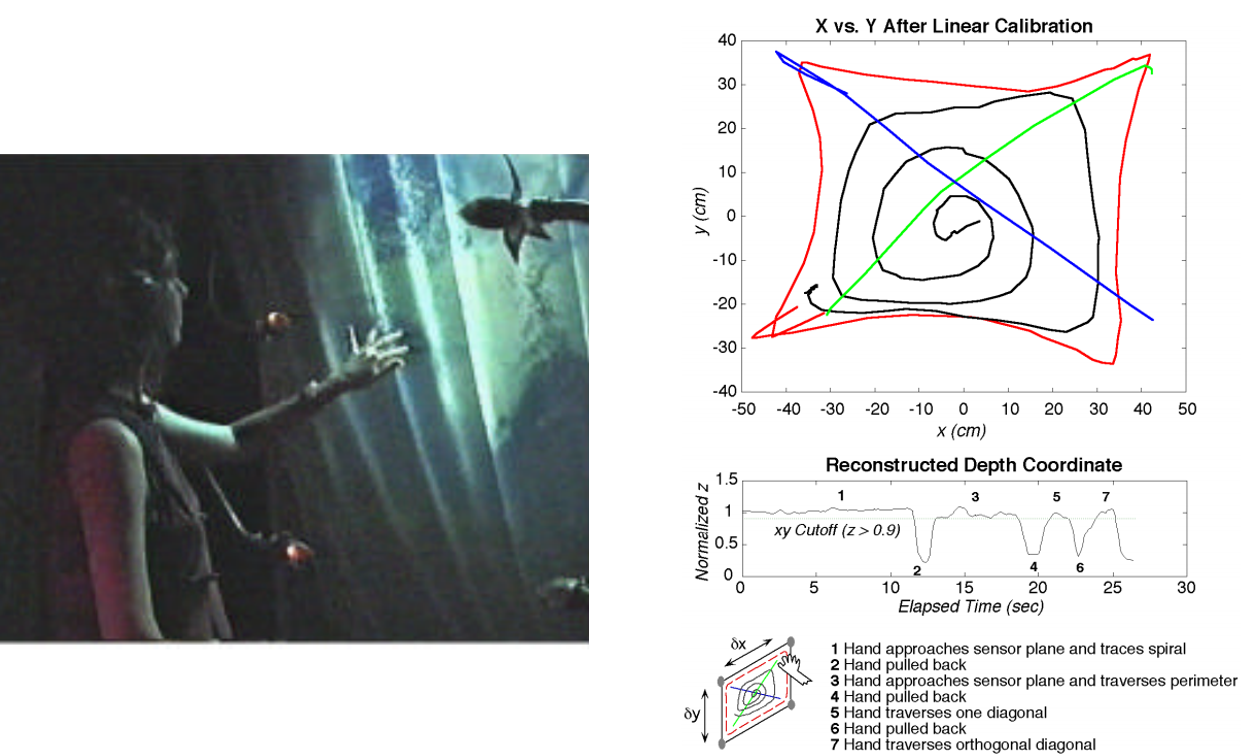
\includegraphics[width=0.8\textwidth]{images/related_gesture_wall}
\captionof{figure}{\emph{Left:} Person interacting with the gesture wall  \emph{Right:} Air drawing results, depth estimation results and associated movements on bottom. \cite{smith1998electric}}
\label{fig:related_gesture_wall}
\end{minipage}

A final prototype of this group I would like to present is the Gesture Wall, a large interactive multimedia wall, designed for public appearances \cite{smith1998electric}. A plate on the floor in front of the screen is acting as transmitter and four receiving electrodes that protruded from the edges of the projection area, as shown in Figure \ref{fig:related_gesture_wall}. It supports interactive experiences, such as drawing in the air, controlling different audio streams and an interactive video clip.

\begin{minipage}{\linewidth}
\centering
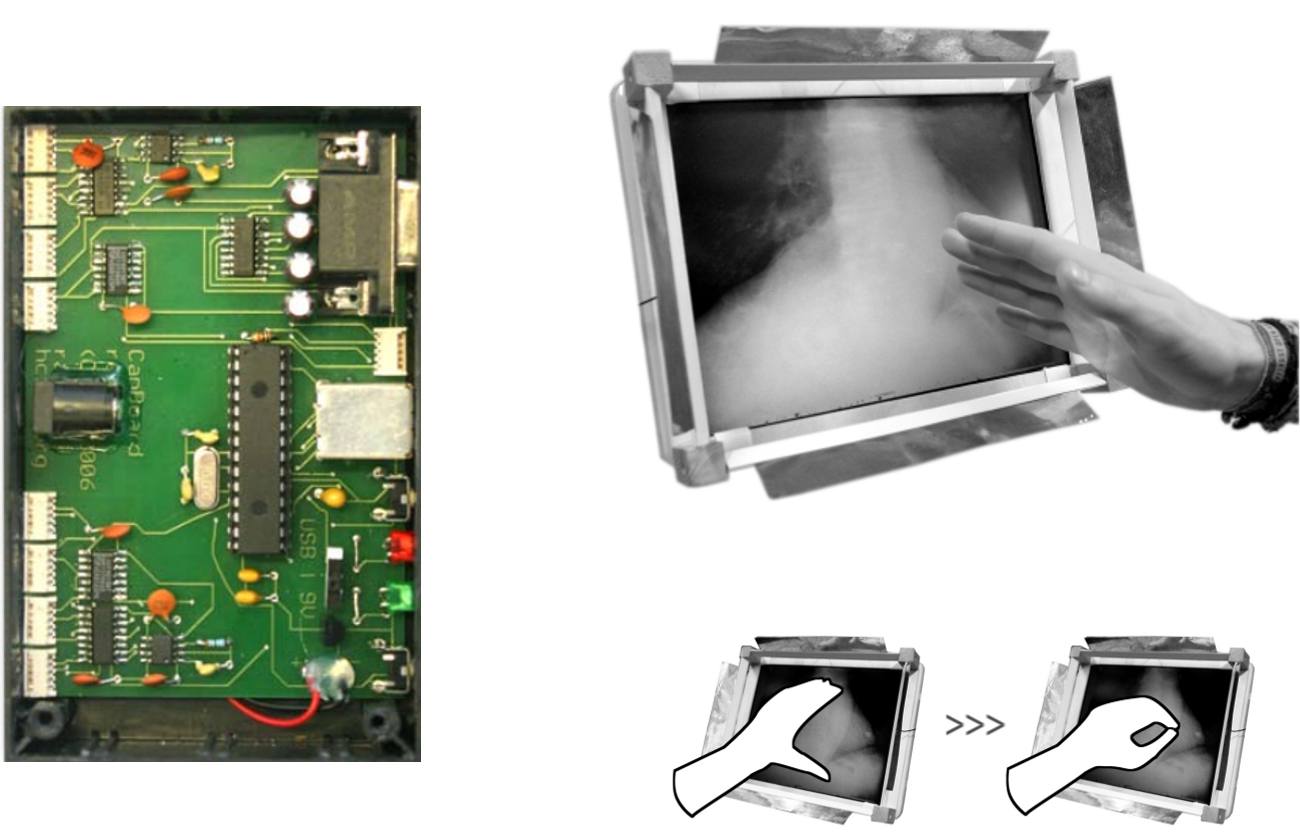
\includegraphics[width=0.9\textwidth]{images/related_ctk_thracker}
\captionof{figure}{\emph{Left:} Prototype of CapToolKit  \cite{Wimmer2007a} \emph{Right:} Thracker prototype and visualized grasping gestures. \cite{Wimmer2006}}
\label{fig:related_ctk_thracker}
\end{minipage}

Another group that was active in capacitive proximity sensing was located at the University of Munich. Raphael Wimmer and colleagues revisited capacitive sensors in the scope of human-computer interaction. They created CapToolKit, a capacitive sensing rapid prototyping toolkit that allows interfacing eight capacitive proximity sensors and enables a quick design and testing of new applications  \cite{Wimmer2007a}. They also created Thracker - a display augmented with four capacitive proximity sensors that allows to detect the position of the hand in front of the screen and supports performed pick-and-drop gestures \cite{Wimmer2006}. Both devices are shown in Figure\ref{fig:related_ctk_thracker}.

\begin{minipage}{\linewidth}
\centering
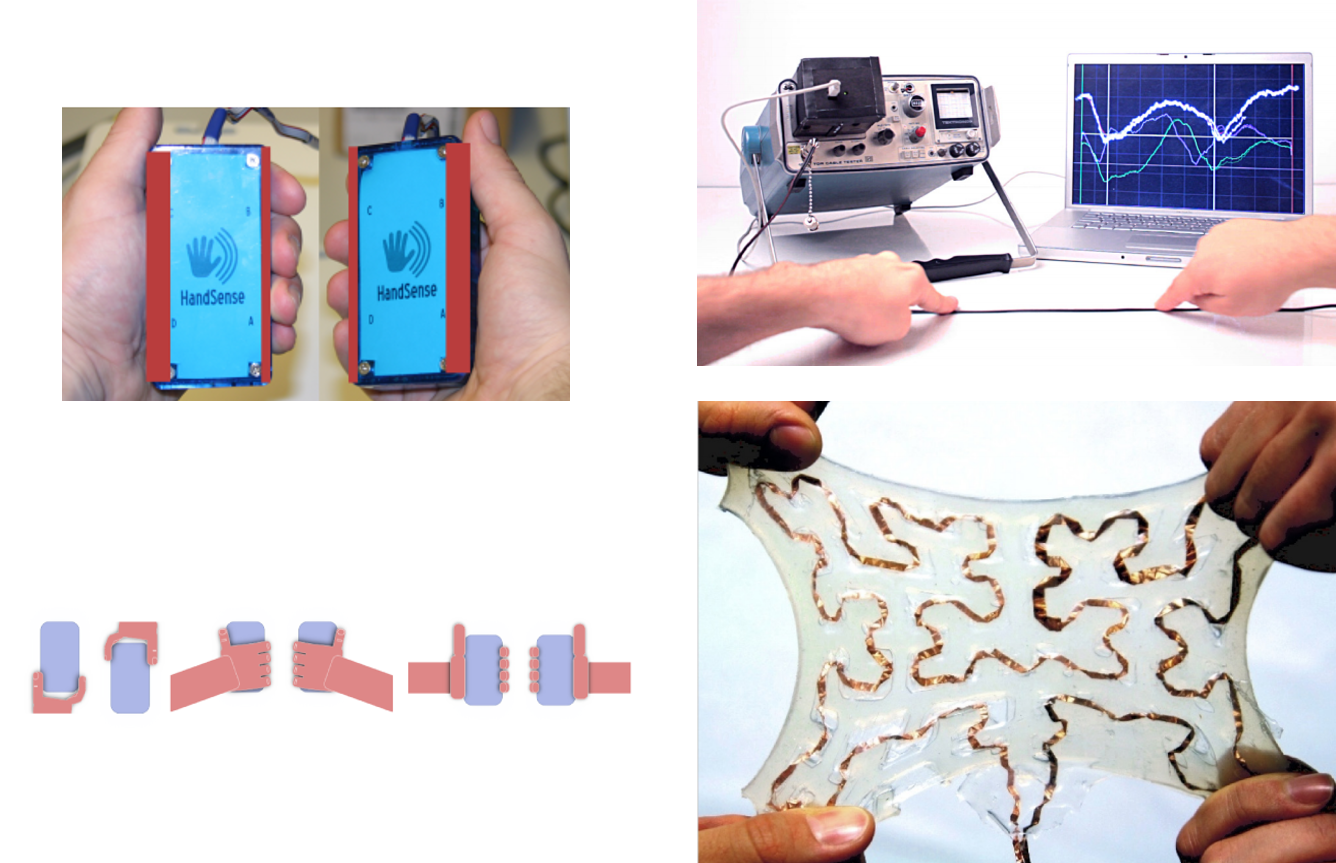
\includegraphics[width=0.8\textwidth]{images/related_handsense_tdr}
\captionof{figure}{\emph{Left:} Prototype of HandSense and supported grasping types \cite{wimmer2009handsense}. \emph{Right:} Setup of time domain reflectometry sensing and example of stretchable material \cite{wimmer2011modular}.}
\label{fig:related_handsense_tdr}
\end{minipage}

In other works they also presented capacitive sensing to allow discriminating the ways an interaction device is held, including distinguishing left and right hand or proximity to a body part \cite{ wimmer2009handsense}. This enables graphical interfaces to be adapted, based on user-handedness, grasping style and spatial cues that can be acquired from this device in collaboration with other sensors. Supported grasping styles and a prototype are shown in Figure \ref{fig:related_handsense_tdr}, on the left.

A final work of this group was concerned with exploring the potential of time domain reflectometry for human-computer interaction \cite{wimmer2011modular}. This technique is sending a short electrical pulse into an electric conductor and measures the time until the signal returns. Originally intended for finding defects in long cables, such as transatlantic phone lines, high-sampling rates enable to also detect the presence of grounding objects close to much shorter conductors. Wimmer and Baudisch use an image analysis on the screen of an older reflectometer to enable applications, such as location tracking, touch detection and stretchable materials. The setup and an example of stretchable materials are shown in Figure \ref{fig:related_handsense_tdr}, on the right.

\begin{minipage}{\linewidth}
\centering
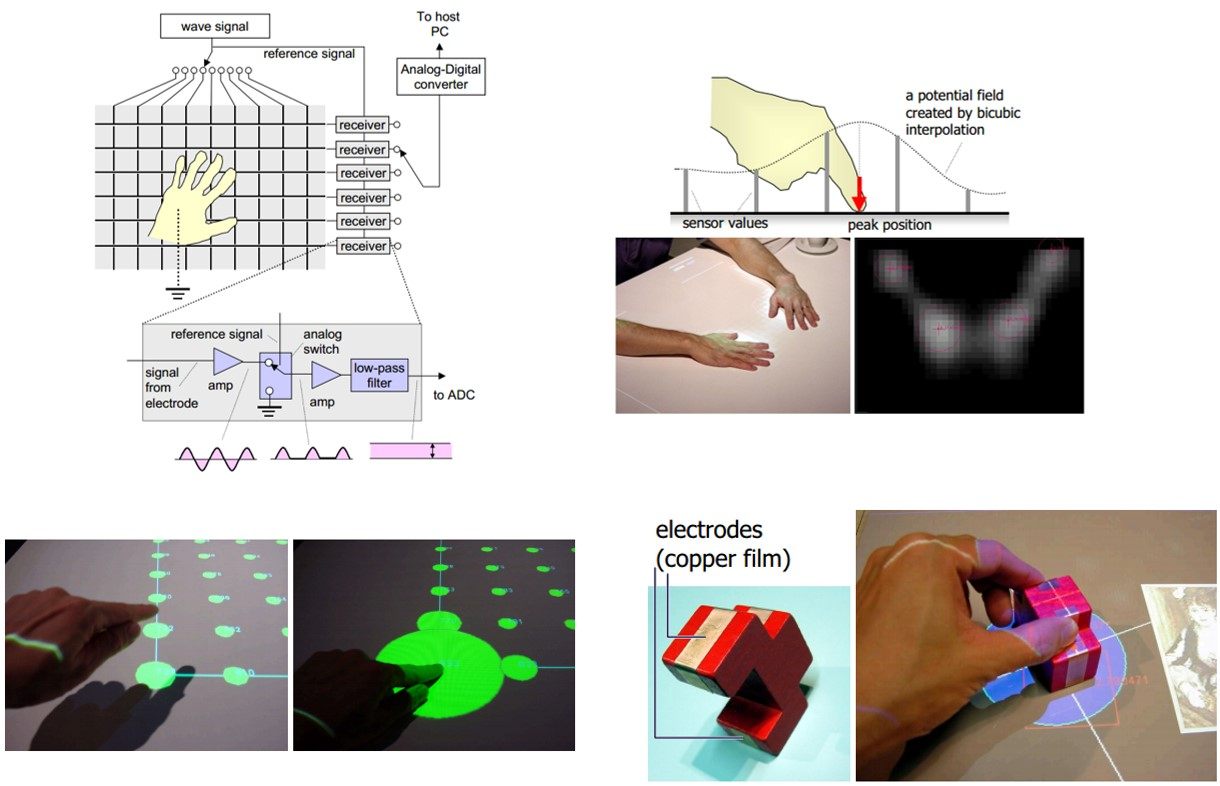
\includegraphics[width=0.8\textwidth]{images/capapp_smartskin}
\captionof{figure}{\emph{Top left:} Technical configuration of SmartSkin. \emph{Top Right:} Bicubic interpolation method to detect the peak of the potential field created by hand proximity. \emph{Bottom left:} Visualized sensor effect of hand hovering in 10 cm distance and touching the surface. \emph{Bottom right:} Capacitance tag having a specific conductive pattern that can be identified \cite{rekimoto2002smartskin}} 
\label{fig:capapp_smartskin}
\end{minipage}

Jun Rekimoto presented SmartSkin, an interactive table based on capacitive proximity sensing based on a number of sensors configured in shunt mode \cite{rekimoto2002smartskin}. They are able to detect hands and fingers at a distance of up to 10 cm, the sensor response being shown in Figure \ref{fig:capapp_smartskin} on the bottom left. He investigated two different prototypes based on this technology and developed an image-based method to detect the position of hand or fingers above the surface, as shown in Figure \ref{fig:capapp_smartskin} on the top right. Additionally, capacitive tags were introduced that enable tangible interaction by detecting the type of object the user is currently touching on top of the surface, analyzing their specific capacitance pattern, resulting from a difference in shape and layout of conductive material covering the object, shown in Figure \ref{fig:capapp_smartskin} on the bottom right.

\begin{minipage}{\linewidth}
\centering
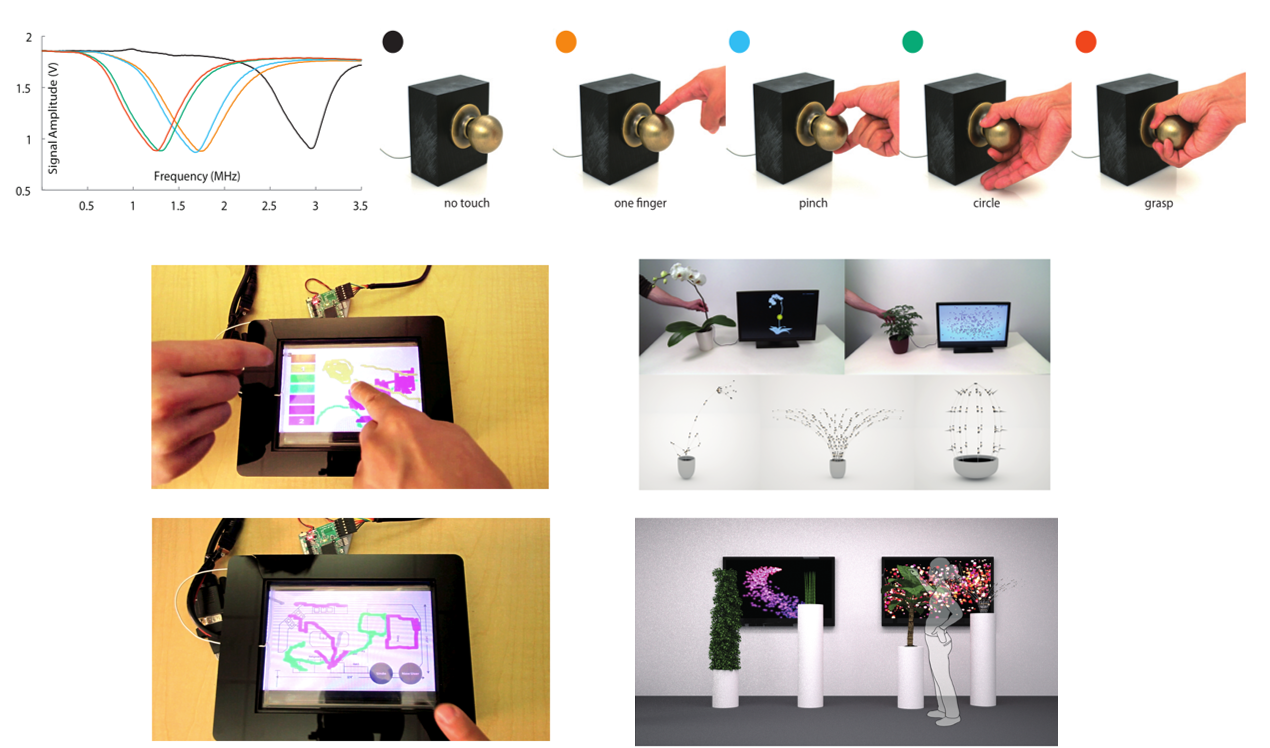
\includegraphics[width=0.8\textwidth]{images/rel_cap_disney}
\captionof{figure}{\emph{Top:} Capacitive profiles of different gestures on a door knob \cite{Sato2012}. \emph{Bottom Left:} User identification using capacitive fingerprinting \cite{harrison2012capacitive}. \emph{Bottom Right:} Botanicus Interacticus prototype and interaction concept \cite{poupyrev2012botanicus}} 
\label{fig:rel_cap_disney}
\end{minipage}

Another research group that has been recently active with capacitive sensing systems is centered around Ivan Poupyrev. They presented Touché, proposing a novel sensing technology called swept-frequency capacitive sensing \cite{Sato2012}. Instead of relying on a single excitation frequency like typical capacitive sensors this measurement system is sweeping a larger range of frequencies, thus allowing to get more data points from a single electrode. Many systems react differently to changing frequencies, including the human body and its complex structure of bone, muscle, fat and other tissues. The result is a capacitive profile comprised of values at different frequencies, as shown in Figure \ref{fig:rel_cap_disney} on the top. Using these profiles it is possible to distinguish numerous events based on the application, e.g. the different ways in which a mobile device can be held. Other applications proposed in this work were sensing of body postures on a table, on-body gestures using wrist-worn sensors, interaction with a body of water and grasping a door knob using different gestures. Building on this work Harrison et al. proposed a system using this technology to identify the users of a touch screen with a capacitive fingerprint \cite{harrison2012capacitive}. This allows to distinguish the touches of different users, thus enabling a variety of applications on collaboratively used touch screen devices, such as gaming and multiuser drawing tools, as shown in Figure \ref{fig:rel_cap_disney} on the bottom left. An interesting suggestion are personalized undo stacks that allow a more seamless collaboration. A final system is the Botanicus Interacticus, that uses the same technology to realize interactive installations using plants  \cite{poupyrev2012botanicus}. It is possible to distinguish the location a certain plant is touched and associate it to different input events. In this first system it was used in an interactive art installation, that is shown in Figure \ref{fig:rel_cap_disney} on the bottom right.

\begin{minipage}{\linewidth}
\centering
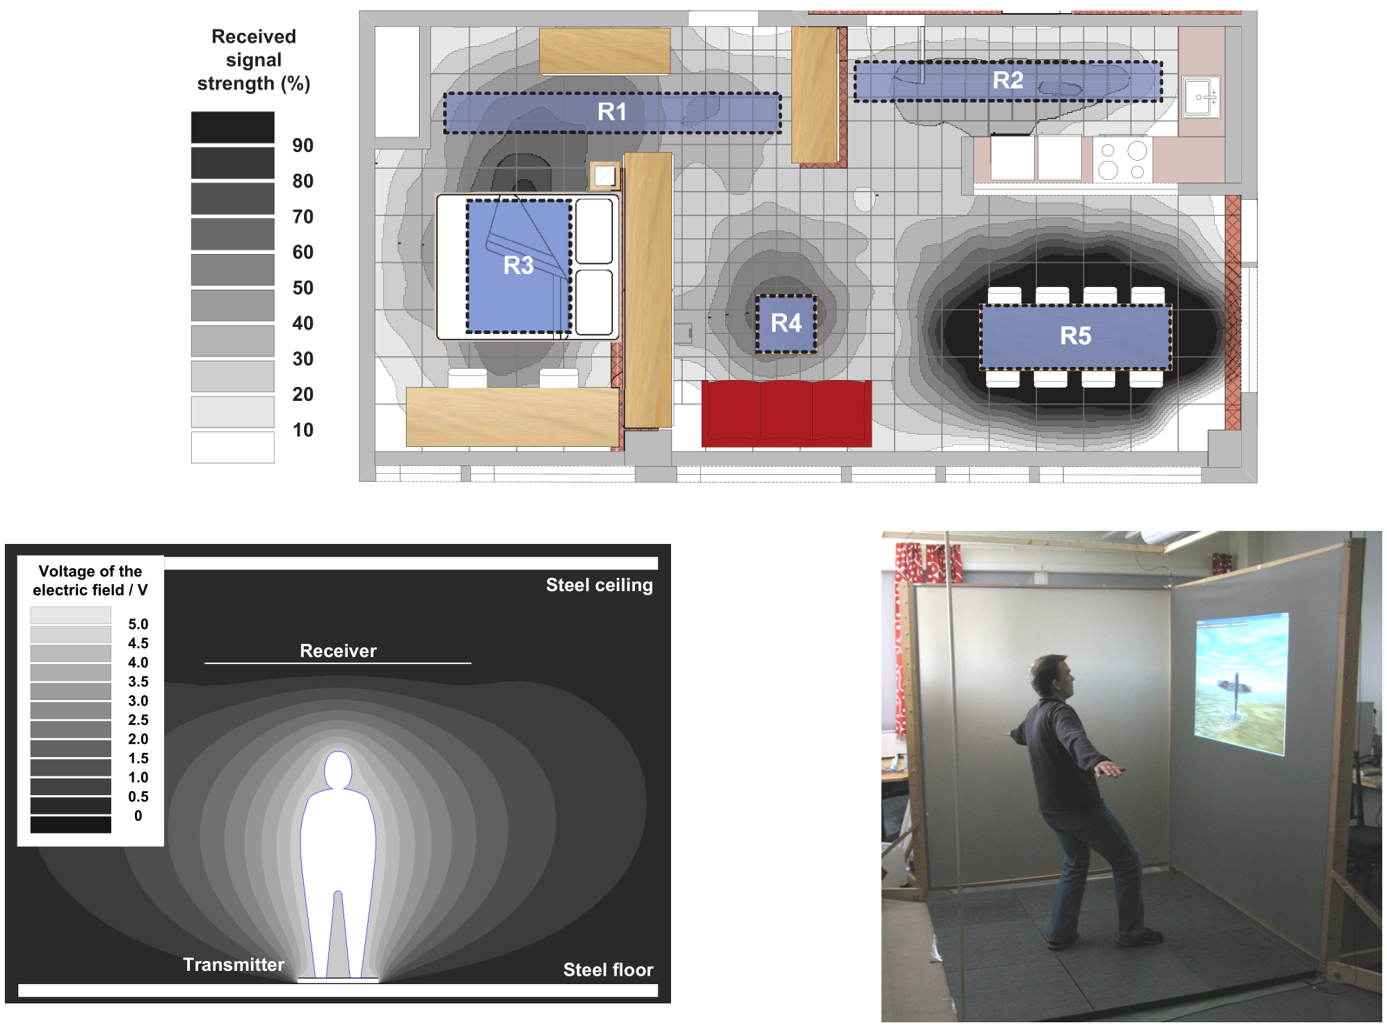
\includegraphics[width=0.8\textwidth]{images/rel_cap_tampere}
\captionof{figure}{\emph{Top:} Capacitive profiles of different gestures on a door knob \cite{Sato2012}. \emph{Bottom Left:} User identification using capacitive fingerprinting \cite{harrison2012capacitive}. \emph{Bottom Right:} Botanicus Interacticus prototype and interaction concept \cite{poupyrev2012botanicus}} 
\label{fig:rel_cap_tampere}
\end{minipage}

A final research group working with capacitive proximity sensing that I would like to present is located at the Tampere University of Technology. Valtonen et al. have been working on a capacitive proximity sensing system tracking the position of users in a room \cite{Valtonen2009a,valtonen2012capacitive}. A transmitting electrode is placed under the floor and several receiver electrodes are hidden in the walls or other objects of the room. The system therefor is using the presented transmit mode, coupling the users present in the environment to an electrode in the floor and measuring the effect on the receiver electrodes. A downside of this system is the required proximity to a wall electrode, making application in larger rooms impossible. Accordingly, an addition was presented that hides the receiving electrodes in different items of furniture to provide a more reliable localization in living environments \cite{valtonen2012capacitive}. The placement of the receiver electrodes (R) and the received signal strength in the environment are shown in Figure \ref{fig:rel_cap_tampere} on the top. An extension of this principle is using a similar electrode configuration to  determine height and posture of a person between a transmitter electrode on the bottom and a receiver electrode on the ceiling \cite{valtonen2011unobtrusive}. A simulation of the electric field voltages created in this setup is shown in Figure \ref{fig:rel_cap_tampere} on the bottom left. The taller a person, the higher the resulting signal. Accordingly, a sitting or lying person will have a much smaller effect and can be classified. A similar setup was also used to identify different gestures performed in an interaction area, as shown in Figure \ref{fig:rel_cap_tampere} on the bottom right \cite{valtonen2010human}. Using a single transmitter and four wire receivers in the corners it is possible to track different body postures and control some example applications.

\begin{minipage}{\linewidth}
\centering
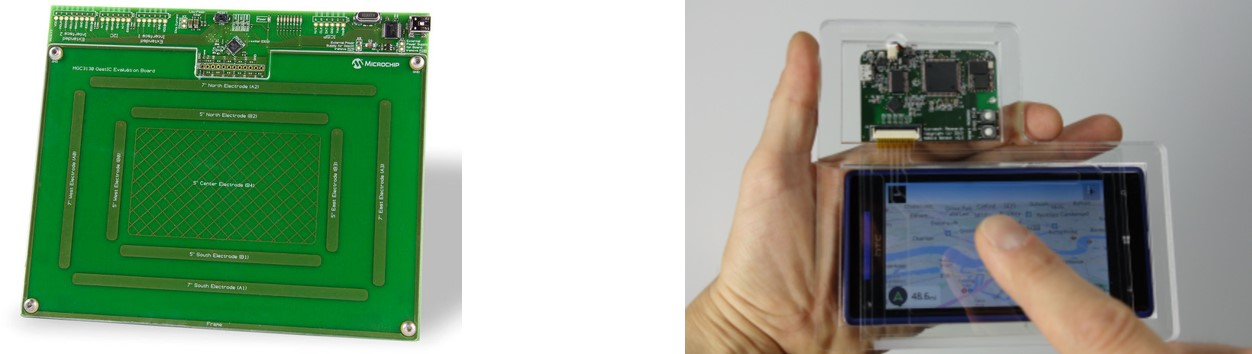
\includegraphics[width=0.8\textwidth]{images/cap_gestic}
\captionof{figure}{\emph{Left:} GestIC sabrewing prototyping board \cite{microchip2013}. \emph{Right:} Transparent interaction device based on GestIC \cite{le2014low}} 
\label{fig:cap_gestic}
\end{minipage}

Recently capacitive gesture interaction has also captured the interest of industry. GestIC by Microchip Technologies Inc. is a controller for electric near field 3D tracking based on capacitive proximity sensing \cite{microchip2013}. A prototyp1ing board is shown in Figure \ref{fig:cap_gestic} on the left. Using a set of several electrodes and on-board processing it is capable of tracking the 3D position of a hand and provides gesture recognition at a distance between 0 and 15 cm. It is based on shunt mode sensing and has a number of different available electrode configurations. This system was used in a recent publication by Le Goc et al. \cite{le2014low}. They used a transparent ITO electrode configuration mimicking the prototyping board configuration and presented a novel machine learning method, that improves the precision of the object localization. They presented a prototype system, augmenting a mobile device with 3D gesture interaction, as shown in Figure \ref{fig:cap_gestic} on the right.




\section{Sensor systems in smart environments}
\label{ch:rel_sensor_tech}
In the most general definition a sensor is a device that transforms a physical property into an observable signal. This definition includes traditional systems such as mercury-based thermometers or hair-based hygrometers. Yet nowadays we are usually considering digital sensors that transfer the measured property to a binary signal that can be further processed by computing devices. 
A common variety is the smart sensor that provides additional functionality beyond generating a correct sensing signal \cite{frank2013understanding}. The main goal is to simplify installation and maintenance of distributed sensing systems by having processing close to the measurement device. Early considerations in this domain were put to the standard family IEEE 1451 - IEEE Standard for a Smart Transducer Interface for Sensors and Actuators between 1997 and 2007 \cite{ieee1451}. An additional concept is the Virtual Sensor that includes digital signal processing and conditioning and therefor abstracts the processing steps from devices interfacing the sensor. 
The number of available sensors is very high, but it is possible to restrict them based on application domain. Lewis and Cook et al. \cite{lewis2004wireless,cook2007smart} have proposed a collection for smart environments focused on wireless sensor networks. The overview is shown in table \ref{tab:sen_smart_env}.
\begin{table}[htbp]
  \centering
  \caption{Sensors for smart environments \cite{cook2007smart}}
    \begin{tabular}{rr}
    \toprule
    \textbf{Properties } & \textbf{Measurand} \\
    \midrule
    Physical properties  & Pressure, temperature, humidity, flow \\ \addlinespace
    Motion properties  & Position, velocity, angular velocity, acceleration \\ \addlinespace
    Contact properties  & Strain, force, torque, slip, vibration \\ \addlinespace
    Presence  & Tactile/contact, proximity, distance/range, motion \\ \addlinespace
    Biochemical  & Biochemical agents \\ \addlinespace
    Identification  & Personal features, RFID or personal ID \\
    \bottomrule
    \end{tabular}%

  \label{tab:sen_smart_env}%
\end{table}%
This sensor categorization is based on the property to be measured and is agnostic to the specific measurement technology. Physical properties, such as pressure, temperature, humidity and flow, can also be noted as environmental properties. They are measurements that determine the state of the smart environment, e.g. temperature in different rooms, or the current water usage. Motion properties denote the movement parameters of actors in this environment and can refer to both humans and machines. Angular velocity is important in self-localization of robots in an environment. Contact properties groups the different types of interaction between surfaces in the smart environment and actors. Presence as a group is similar to motion paramteres, but does not require a series of measurements for tracking an actor. Biochemical sensors enable measuring the presence of specifc chemical compounds in the environment and are most suited for measuring pollution or air quality. Finally, identification of actors allows to provide personalized services and can be realized with different methods ranging from tags to biometric systems.

While this listing provides a decent overview of sensing properties in smart environments it is abstracted from sensor technologies. Various types of sensors, including capacitive proximity sensors, allow us to detect multiple of these properties and thus providing a higher flexibility. Therefore it is possible to provide an inverse listing of sensor technologies that allow measuring different properties. A short overview of sensor technologies with this capabilities and that are commonly used in smart environments is given in table \ref{tab:sen_tech_prop}. In the following sections I want to give an overview on how these sensor systems are used in this domain, in order to provide a basis for the benchmarking model that will be introduced in section \ref{ch:benchmark}.
\begin{table}[htbp]
  \centering
  \caption{Sensing technologies and measured properties}
    \begin{tabular}{rr}
    \toprule
    \textbf{Technology} & \textbf{Properties} \\
    \midrule
    RGB cameras  & Motion, Presence, Identification \\ \addlinespace
    Infrared cameras & Motion, Presence, Contact \\ \addlinespace
    Ultrasound sensing & Motion, Presence, Contact, Identification \\ \addlinespace
    Microphone arrays & Motion, Presence, Contact, Identification \\ \addlinespace
    Radiofrequency sensing & Motion, Presence, Identification \\
    \bottomrule
    \end{tabular}%
  \label{tab:sen_tech_prop}%
\end{table}%

\subsection{RGB cameras}
\begin{figure}[h]
\centering
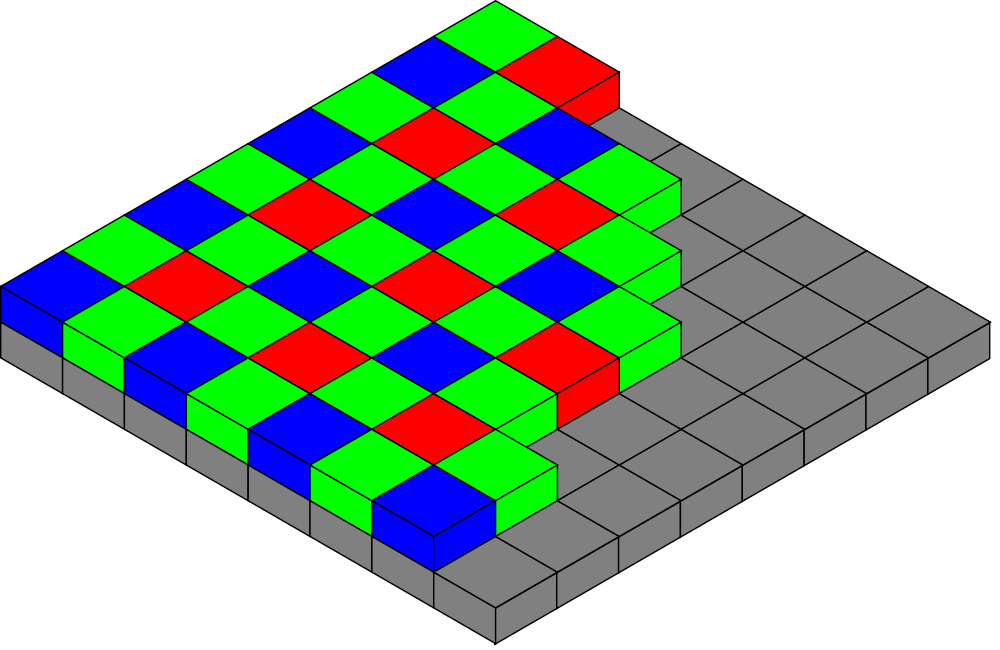
\includegraphics[width=0.4\textwidth]{images/bayer_pattern_on_sensor}
\caption{A bayer pattern on a sensor in isometric perspective \cite{img_bayer_pattern}}
\label{fig:bayer_pattern}
\end{figure}
A RGB camera is an image processing device that processes light in the visible spectrum, similar to the human eye. Modeled after the retina it has three distinct color channels - red, green and blue. There are different methods available to distinguish these channels from visible light, such as Bayer filters (Figure \ref{fig:bayer_pattern}) in front of a single sensor or using multiple sensors behind a prism.
The usage of cameras in smart environments is very common. I will present five different examples and afterwards will specify how they are linked to the properties that were defined previously.
Tabar et al. have been using a combined system of cameras, RF transmitters and wearable sensors in a home care scenario \cite{tabar2006smart}. The cameras are used to improve the accuracy of the accelerometer-based fall detection by eliminating false positives. Once a fall event occurs an algorithm tracks the posture of detected humans in the scene (Figure \ref{fig:rel_tech_body_face} - left). They used an edge detector to distinguish the human body from other objects and applied a heuristic to differentiate lying and standing.  Additionally a face detector was used to improve the recognition of human objects. Combining this with information from the fall detecting sensor and a RF based localization system they were able to achieve a good reliability in eliminating false positive alerts.
\begin{figure}[h]
\centering
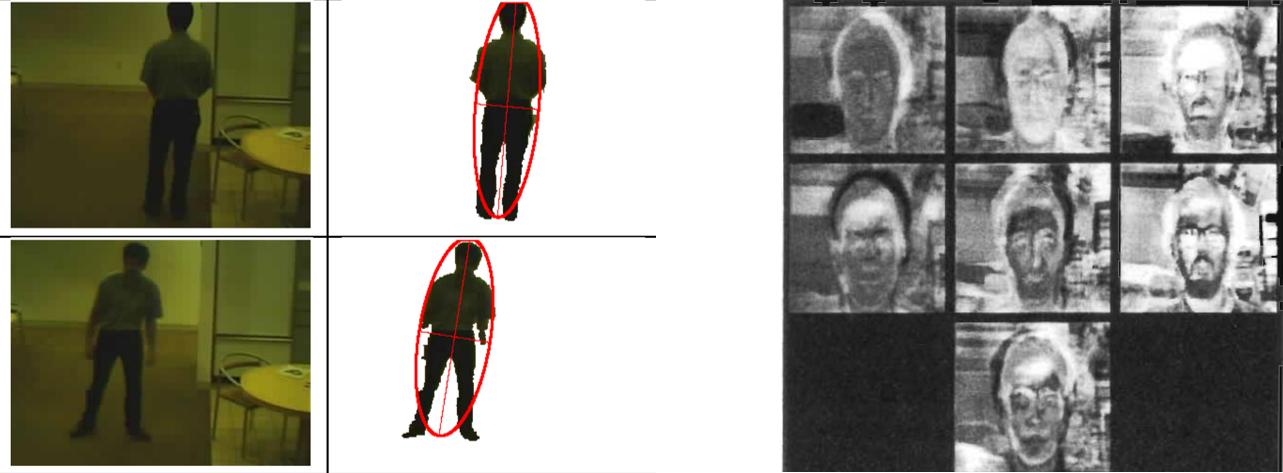
\includegraphics[width=0.9\textwidth]{images/rel_tech_body_face}
\caption{\emph{Left}: Tracking of body masks using cameras  \cite{tabar2006smart}. \emph{Right}: Eigenfaces created from input picture set \cite{pentland2000face}}
\label{fig:rel_tech_body_face}
\end{figure}

Pentland and Choudhury provided an overview of vision-based face recognition systems in the domain of smart environments \cite{pentland2000face}. The systems are able to identify users and recognize facial expressions. The proposed applications in smart environments include personalized shopping experiences based on customer recognition, behavior monitoring in child care facilities and emotion-aware systems that react to the user's current awareness. The described techniques include PCA-supported, eigenvector-based classification, face-based localization and systems based on local feature analysis (Figure \ref{fig:rel_tech_body_face} - right). Newer systems are able to operate well in unconstrained environments, that include varying expression and illumination, ageing of persons, occlusion and disguise \cite{wright2009robust}.
\begin{figure}[h]
\centering
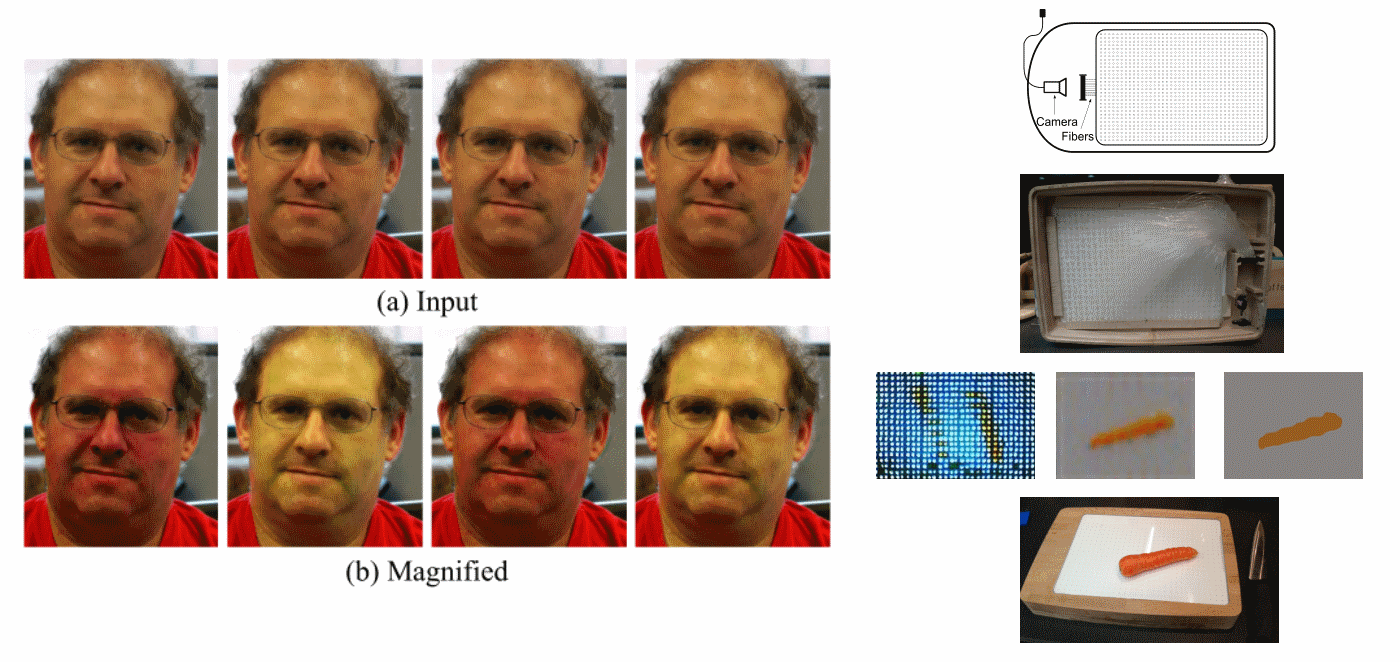
\includegraphics[width=0.7\textwidth]{images/rgb_euler_food}
\caption{\emph{Left}: Eulerian Video Magnification to attenuate the human pulse with original (a) and amplified (b) video sequence  \cite{Wu2012}. \emph{Right}: FoodBoard schematics (top), underside view (second row), original, reconstructed and segmented image (third row) and final system (bottom) \cite{pham2013foodboard}}
\label{fig:rgb_euler_food}
\end{figure}

An example for a novel image processing method that is useful in smart environments was presented by Vu et al. in 2012 \cite{Wu2012}. They are using  temporal variances of pixel values to exaggerate spatial movements and color changes that would typically be invisible to the naked eye. The method is called Eulerian Video Magnification and uses a combination of spatial decomposition and temporal filtering applied to adjacent frames. It can be tuned to different time-frequency bands to attenuate different classes of signals. Some of the proposed applications include the tracking of breathing rates of infants by attenuating chest movement, or the tracking of subtle movements, such as vibration in appliances. The example shown in Figure \ref{fig:rgb_euler_food} on the left is using a magnification of colors, in order to identify the heart rate of a person. The latter can be used for personal health applications, e.g. by integrating the system into the bath room mirror to provide an unobtrusive daily measurement and give the user feedback over a longer period of time.

A final example in this section is the FoodBoard, a smart chopping board that uses image processing to recognize the food items that are put on it \cite{pham2013foodboard}. It is shown in Figure \ref{fig:rgb_euler_food} on the right. To enable a thin footprint, ambient light is transferred to a camera using glass fibers. The picture is reconstructed and segmented, allowing to identify different items of food that are placed on it. The classification is based on a combination of Fast-Hessian and color histogram feature extractors. Pham et al. were able to distinguish 12 different ingredients with an accuracy between 59\% and 93\%. The system can be used to support dietary monitoring, give recipe guidance or support visually impaired users in identifying and tracking food.
\subsection{Infrared cameras}
\begin{figure}[h]
\centering
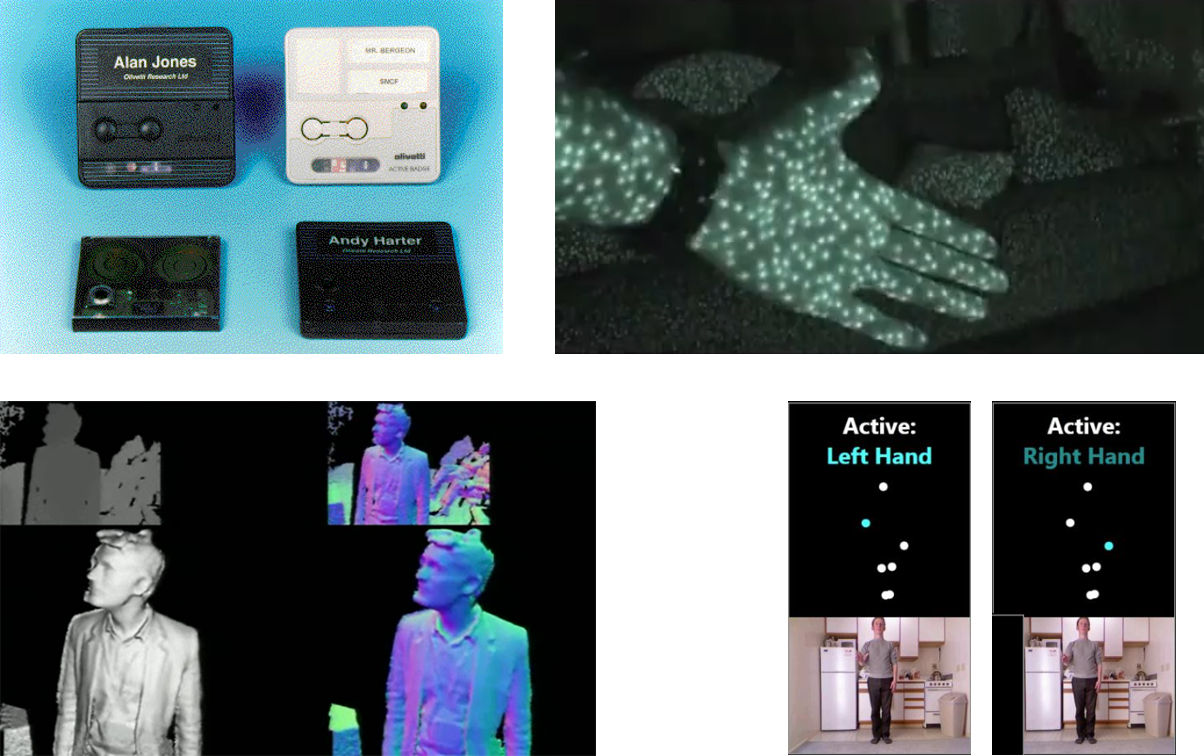
\includegraphics[width=0.9\textwidth]{images/rel_tech_infra}
\caption{\emph{Top Left}: ORL Active Badge  \cite{Weiser1991}. \emph{Top Right}: Kinect infrared projection \cite{zhang2012microsoft}. \emph{Bottom Left}: Kinect Fusion reconstrucion  \cite{Izadi2011}. \emph{Bottom Right}: Kinect kitchen interaction \cite{panger2012kinect}}
\label{fig:rel_tech_infra}
\end{figure}
Infrared imaging is using the same sensors that are suitable for visible light imaging. The difference is that they are tuned to collect electromagnetic waves of a lower wavelength that are just outside of the visible spectrum. This allows for distinct applications, such as thermal imaging, as it is possible to detect heat radiation. One of the earliest prototypes in Ubiquitous Computing designed by PARC was using the ORL Active Badge, an infrared emitter developed by Olivietti Research Laboratories that was used to identify persons operating in the environment \cite{Weiser1991} (Figure \ref{fig:rel_tech_infra} Top Left). In smart environments the most common application is using infrared cameras in combination with infrared light sources. This allows to illuminate spaces without visible artifacts to the user, thus providing imaging capabilities in dark rooms, or very specific conditions that may be required by a certain application. Another very interesting option is to use a specific projection of patterns into the scene. Analyzing the returning infrared light it is possible to infer the depth of specific pixels of the camera (Figure \ref{fig:rel_tech_infra} Top Right). This variety is called a depth camera. Particularly in the last few years the research in this domain has expanded strongly, sparked by the availability of an affordable depth camera/RGB camera combination - the Kinect by Microsoft \cite{zhang2012microsoft}. On the following pages we will present various examples of how this device can be used in smart environments to enable different applications in interaction and activity tracking.

Sung et al. have presented a system that is tracking activities of daily life based on the movements of a skeleton that is provided by the Kinect API \cite{sung2011human}. This skeleton model is based on a pose reconstruction algorithm developed by Shotton et al. \cite{Shotton2013} and is used in many different Kinect-based applications. The algorithm is using a method called hierarchical maximum entropy Markov model (MEMM). Each activity is considered to be composed of sub-activities. Based on this assumption a two-level graph is generated using dynamic programming. The system was tested with twelve activities performed in an office, a kitchen, a living room, a bathroom and a bedroom. If the person was part of the training set the precision was 84.3\% and 64.2\% for unknown persons. Some example activities of the acquired dataset are shown in Figure .

A novel method to use the Kinect for fast 3D reconstruction of scenes was presented by Izadi et al. in 2011 \cite{Izadi2011} (Figure \ref{fig:rel_tech_infra} Bottom Left). The basic premise is to use a fast registration method to combine point clouds that are generated by the system and continuously extend and optimize the current model of the scene. They are using a GPU-based ICP implementation to track the position of the camera in six degrees-of-freedom. This allows to reliably integrate the different point clouds into a single voxel grid that can be used to represent and render the scene. They proposed a number of applications ranging from phyiscal simulation of particles in the scene, to system control based on segmenting and tracking the user's hands and their interaction with arbitrary surfaces in the environment. Figure  shows some results of the touch recognition in a reconstructed scene.

Galen has presented a method to use a Kinect in a kitchen to provide touch free interaction \cite{panger2012kinect}. Two different interaction schemes are proposed. The first allows to control the applications with messy hands, the second enables to use other limbs if the hands are currently occupied (Figure \ref{fig:rel_tech_infra} Bottom Right). Three different test applications have been implemented. A recipe navigator that allows to open and navigate through different recipes. A timer that enables setting different alarm times, similar to a kitchen clock and a music player that can be controlled to choose different stations according to preference. A real life test with five subjects  did also test installation complexity, which was deemed favorable. There were some concerns in clearly distinguishing commands from random movements performed in the kitchen.

The final system based on infrared cameras is an immersive telepresence system developed by Beck et al. \cite{beck2013immersive}. Telepresence enables persons to be present as a representation in a remote place. A typical example is video conferences, but advanced system may include robotics or virtual elements. The presented system is using a single Kinect for each participant. A 3D representation is created based on the depth information of the infrared camera and on-the-fly texturing using the included RGB camera. The virtual user representations are put into a shared virutal environment and can interact with each other. Some variations were tested where local and remote users were decoupled, side-by-side or face-to-face. Different tracing and pointing gestures are supported. The supported applications included the exploration of a virtual city.

\subsection{Ultrasound sensors}
\begin{figure}[h]
\centering
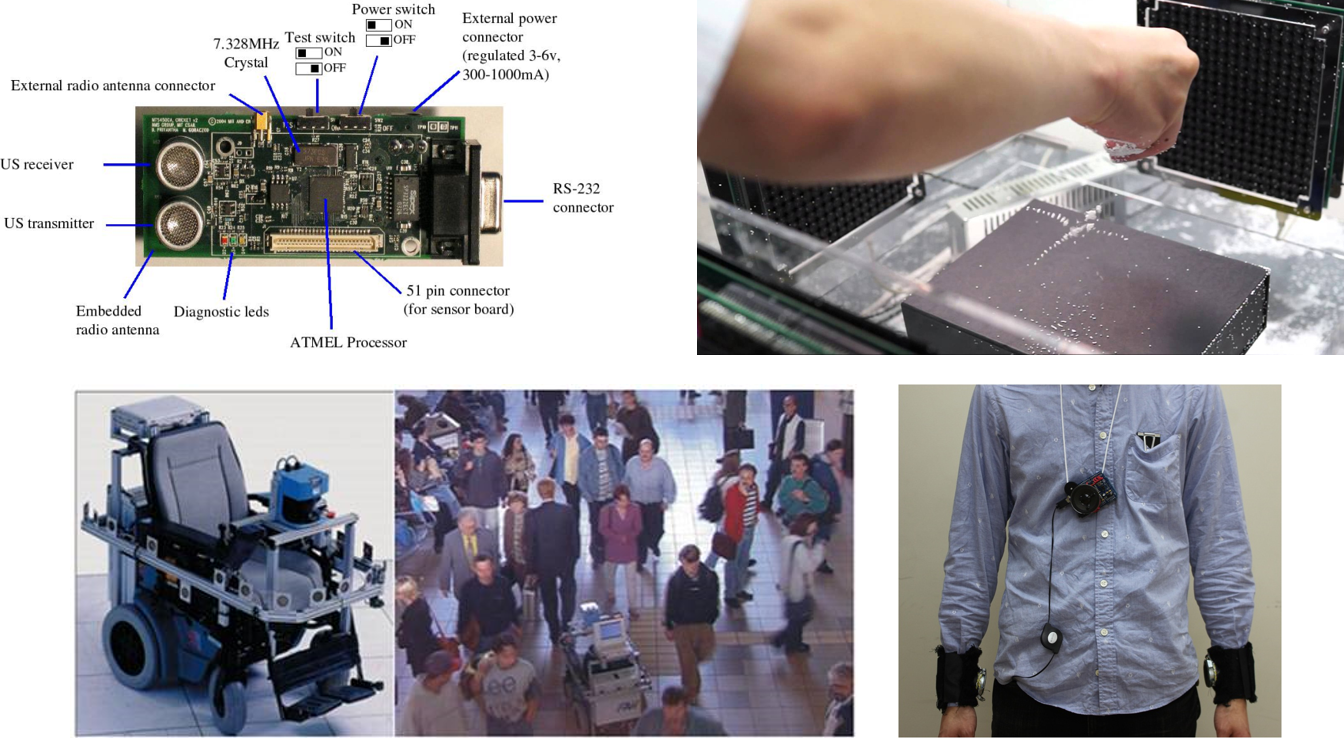
\includegraphics[width=0.9\textwidth]{images/rel_tech_ultra}
\caption{\emph{Top Left}: Cricket Indoor Localization hardware \cite{priyantha2000cricket}. \emph{Top Right}: Mid-air particle manipulation \cite{ochiai2013three}. \emph{Bottom Left}: Robotic wheelchair MAid with ultrasound range sensors \cite{prassler2001robotics}. \emph{Bottom Right}: Activity and context recognition using ultrasound sensors \cite{watanabe2013ultrasound}}
\label{fig:rel_tech_ultra}
\end{figure}
Ultrasound sensors allow detecting sound wave signals that have a frequency beyond 20kHz and are thus not audible to humans. Their propagation and reflection properties are similar to audible sound waves, thus the generated measurements can be similar. While there are natural sources of ultrasound waves the applications in smart environments do rely on active systems, that combine sound generators and sensors that measure the resulting signal. By timing the time distance between sending the signal and receiving a response it is possible to measure distances between the sender and different object.  If various receivers are used it is possible to localize the sound source, making ultrasound sensing a popular candidate in indoor localization systems. In Figure we can see a sketch of the basic functionality of ultrasound sensing systems on the left, and an example of localization using three receivers and a single source. We will present four different examples on how ultrasound sensors are used in smart environment applications.

The Cricket developed by Pryantha et al. is an example for an indoor localization system based on a badge the tracked object has to wear \cite{priyantha2000cricket}. The badge is periodically sending signals to a set of beacons that determine the distance and calculate a location. Initially it was supposed to solely rely on radiofrequency signals, but was modified to use a combination of RF and ultrasound. The rationale of this decision is the considerably slower speed of sound that simplifies measuring the time-of-flight and thus allows for more precise distance measurements. Consequently this also leads to a better precision in the localization algorithm. Additionally, the system uses some novel methods to deal with interference and multipath issues, that is dealing with reflected signals. As potential applications they propose space-dependent services that are provided as the user is identified in a certain region and guidance scenarios on a floor plan. The hardware is shown in Figure \ref{fig:rel_tech_ultra} (Top Left).

The robotic wheelchair MAid (Mobility Aid for Elderly and Disabled People) was designed to support and transport people with limited motion skills \cite{prassler2001robotics}. It is based on a commercial wheelchair that has been equipped with an intelligent control and navigation system. The system includes an ultrasound-based range finder that allows to detect obstacles in the path and circumnavigate around (Figure \ref{fig:rel_tech_ultra} Bottom Left). 

Watanabe et al. investigate the role of ultrasound sensors in recognizing activities and gestures of a user \cite{watanabe2013ultrasound}. The system is comprised of a microphone attached to a necklace and two speakers that are attached to each wrist. Based on the acquired volume and evaluation of the Doppler effect it is possible to determine both distance of the wrists from the neck and the speed of movement (Figure \ref{fig:rel_tech_ultra} Bottom Right). Watanabe et al. want to determine if this system allows for similar performance compared to other body-worn systems based on accelerometer and gyroscope data. Additionally it was evaluated if external microphones can perform as well as the neck worn microphone. The system was able to recognize 87\% of activities and gestures in a set of 10 test persons if no influencing sound was present. The ultrasound did also improve results if environmental noise was present.

A recent project at the University of Tokyo evaluates the potential of ultrasound in manipulating small particles in free-air \cite{ochiai2013three}. Using standing waves to  create sound pressure notes it is possible to apply a force to small particles that is sufficient to counteract gravity. Using a set of ultrasonic phased arrays it is possible to create these sound pressure nodes at arbitrary positions in three dimensions (Figure \ref{fig:rel_tech_ultra} Top Right). Ochiai et al. use this to move small objects around and investigate required object properties and their floating properties. So far the moved items have to be very light and smaller than 2 mm in diameter, resulting in the usage of polystyrene. The technology is also able to hold and move small amounts of fluid. Suggested applications include object manipulation in microgravity environments and projected haptic feedback systems.

\subsection{Microphone arrays}
\begin{figure}[h]
\centering
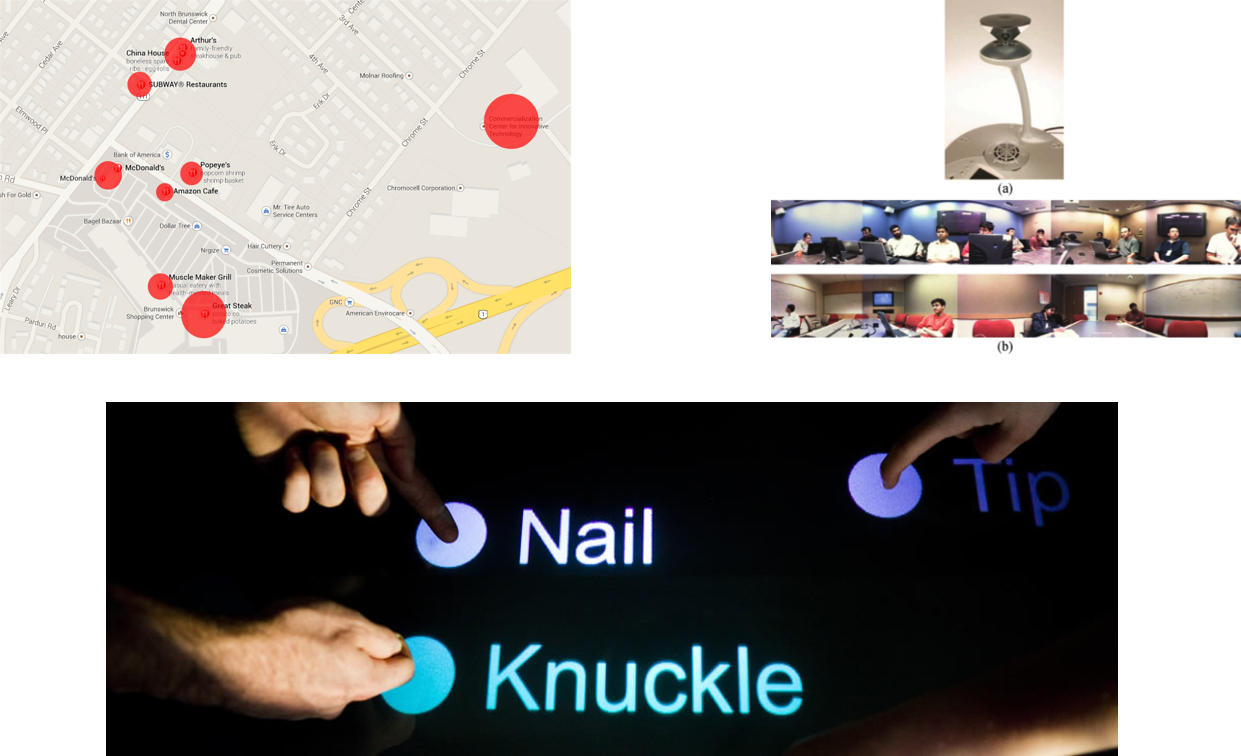
\includegraphics[width=0.9\textwidth]{images/rel_tech_mic}
\caption{\emph{Top Left}: Visualization of speaker count in different areas \cite{xu2013crowd++}. \emph{Top Right}: Directional microphone and conference room for speech source localization \cite{zhang2008maximum}. \emph{Bottom}: TapSense detecting different tap events \cite{harrison2011tapsense}.}
\label{fig:rel_tech_mic}
\end{figure}
Microphones are signal receivers that are tuned to detect sound frequency ranges that are audible by humans. Typically they consist of a piezo element that transfers vibration to an electric current that is amplified. Most human activities produce some kind of sound. As opposed to the presented ultrasound system, microphones typically operate passive. That is there is usually no dedicated signal source, but instead naturally occurring sounds are picked up. By combining microphones or arrays thereof with data processing systems that are aimed at analyzing specific sound patterns we are able to get feedback on human activities. Looking at smart environments there are numerous use cases that can benefit from microphones as sensors. In this section we will present four different systems that cover a large variety of different applications, ranging from breathing rate detection to estimating the number of speakers in large groups.

Detecting the breathing pattern of a person has several applications in smart environments. Apart from medical applications that require detecting abnormal breathing in risk groups it is also possible to track training progress using such a system or provide a measure for the current attention level in affective computing. Corbishley et al. investigated using very small microphones in mobile devices to enable detecting the breathing rate \cite{corbishley2008breathing}. The algorithm is designed to be applicable on single ICs, allowing for miniaturization and energy efficiency. Even with the presence of noise the combined score for true negatives and true positives was as high as 91.3\%. Using small and energy efficient systems also enables unobtrusive applications in non-mobile environments, e.g. placing such a system close to the bed to detect the breathing rate while the user is sleeping.

Collaborative applications are an important aspect of smart environments, e.g. to link together meeting places at different places, similar to the presented telepresence applications. If a multitude of speakers is present it gets increasingly difficult to provide a system that enables proper speech transmission for all participants. Using an array of microphones it is possible to focus the attention on the person currently speaking and filter out environmental noise. A project at Microsoft Research investigated using a maximum likelihood of two known techniques, beamforming and speech source localization, to enable a reliable speaker selection \cite{zhang2008maximum} (Figure \ref{fig:rel_tech_mic} - Top Right). Additionally the framework enables a good adaptation even if directional microphones are used that are placed close to each other. The method provides a real life accuracy of more than 90\%.

A fairly new work was performed by Xu et al. \cite{xu2013crowd++}, called Crowd++. Their idea is to use smartphone microphones to identify the number of speakers in crowded environments. Such system could be used to estimate the number of persons in a given place and potentially react quickly if a crowd panic may occur. The method is based on an unsupervised machine learning classification of short audio parts that are picked up by the individual microphones in the handsets. It was tested by 120 participants in 10 different environments and allowed detecting the number of persons with an average error of 1.5 persons (Figure \ref{fig:rel_tech_mic} - Top Left). No dedicated hardware is required to achieve this precision, enabling an application using off-the-shelf smartphones.

Microphones can also be used to analyze the mechanical surface waves that occur when objects interact with each other. Harrison et al. have designed TapSense, a microphone based sensor system that improves touch interaction by classifying the sounds created by different objects hitting the surface \cite{harrison2011tapsense}. In particular different parts of the hand can be distinguished, including nail, knuckle or tip. Potential applications are improving touch interaction on touch screens by enabling different forms of interaction, but also can be adapted to mobile devices, that typically have less interaction space and increase the expressiveness of different touch gestures. The achievable accuracy was between 95\% using four different input types up to 99\% when using just two input sets, such as finger and pen (Figure \ref{fig:rel_tech_mic} - Bottom).

\subsection{Radiofrequency sensing}
\begin{figure}[h]
\centering
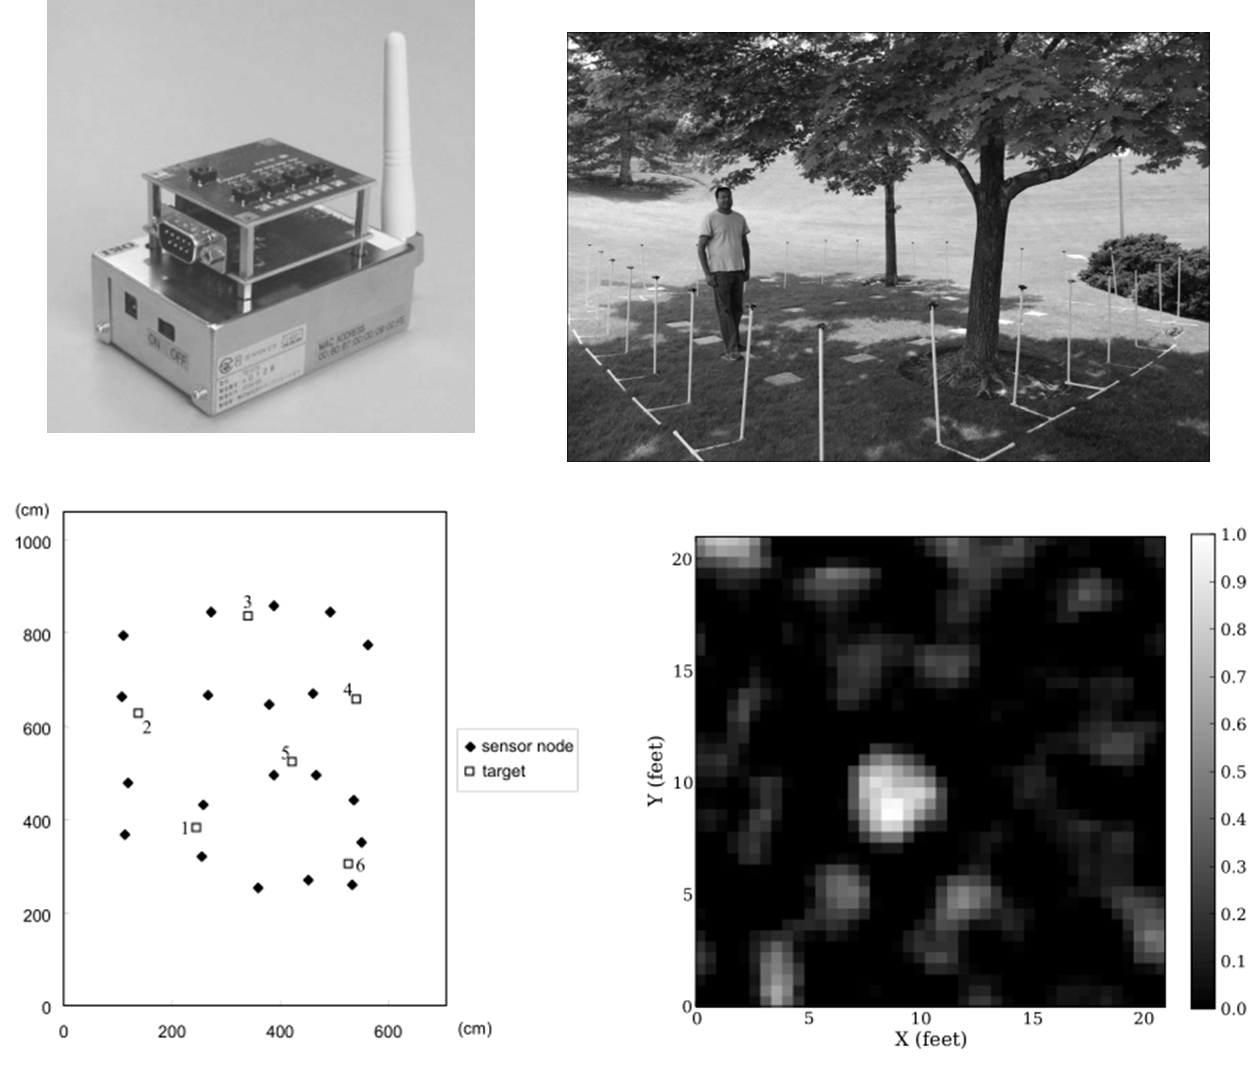
\includegraphics[width=0.9\textwidth]{images/tech_mic1}
\caption{\emph{Top left} ZigBee node. \emph{Bottom Left} Sensors and targets in larger room \cite{sugano2006indoor}. \emph{Top right} Photo of radio tomography setup. \emph{Bottom right} Result attenuated signal \cite{wilson2010radio}.}
\label{fig:tech_mic1}
\end{figure}

Radiofrequency sensing is a traditional field for sensors. Radar is a system that uses radio waves to acquire direction, speed, distance or altitude of objects and was developed at the beginning of World War II. This variety is using active sensing and emits radio waves that are reflected by objects. Most applications in smart environments similarly rely on active systems. A popular signal source are WiFi signals, intended to wirelessly transmit information between several systems. The systems are wide-spread, with all smartphones possesing two or more wireless technologies (typically 4G/3G/GSM for long range communication, WLAN for medium range communication and Bluetooth/NFC for short range communication) that can be used in coordination with stations placed in the environment. The signal processing of the wireless LAN sets generates some additional data that can be used, most notably the signal strength (RSSI). We will present different systems that show some different ways how radiofrequency sensing can be used in smart environments.

Radiofrequency based systems are very popular for indoor localization applications. We previously glimpsed at the difficulty of time-of-flight systems in the electromagnetic specturm. Thus most systems rely on a different approach, using the received signal strength (RSSI). If the initial signal strength is known and we have a good estimate how the signal propagates we can estimate the loss of signal strength at a certain distance. An accepted work that helped shaping this domain is the system created by Sugano et al. in 2006 that uses a ZigBee-based network with a limited number of nodes receiving RSSI information \cite{sugano2006indoor}. Based on this it is possible to locate one or more users with an error between 1.5-2m. This often is sufficient to distinguish the room a person is currently in, enabling a room-based system adaptation, which is suitable for many applications. A photo of a ZigBee node and results in a larger conference room are shown in Figure \ref{fig:tech_mic1} on the left.

A different approach for RSSI based systems was presented by Wilson and Patwari in 2010 \cite{wilson2010radio}. They are using tomography methods to determine the location of users. By placing a large number of sensors on the outer limits of the environment and creating a unique link between each, it is possible to infer the position based on the signal attenuation when a person moves in the environment. The human body absorbs some of the signal, resulting in a reduced received RSSI in the affected nodes. The error for standing persons was between 0.64cm for a single person and 1.10cm for two persons. An image of the test area and the resulting reconstructed attenuation map are shown in Figure \ref{fig:tech_mic1} on the right.

\begin{figure}[h]
\centering
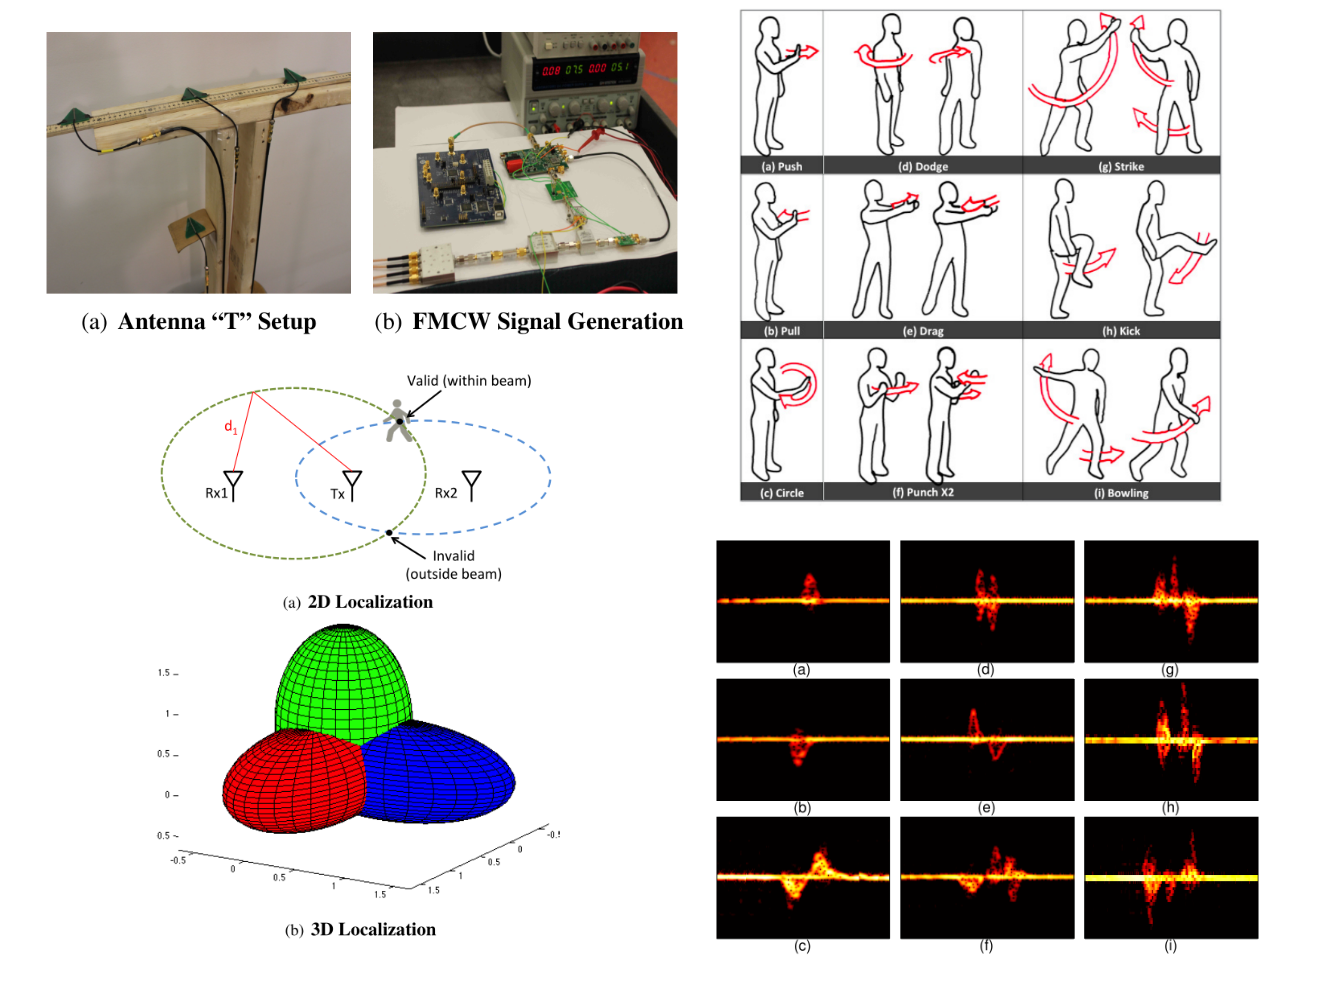
\includegraphics[width=0.9\textwidth]{images/tech_mic2}
\caption{\emph{Top left} WiTrack antennas and signal generator. \emph{Bottom Left} WiTrack 2D and 3D localization method \cite{adib20133d}. \emph{Top right} WiSee supported gestures. \emph{Bottom right} WiSee Doppler profiles of gestures \cite{pu2013whole}.}
\label{fig:tech_mic2}
\end{figure}

A final system that provides a localization is WiTrack, presented by Adib et al in 2013 \cite{adib20133d}. It uses the signal reflected by the human body to provide a location estimate based on time-of-flight. As mentioned previously this is challenging due to the propagation speed within the electromagnetic field. To overcome this issue they are using a method called frequency modulated carrier wave that transfers time differences to the frequency domain. Looking at the spectrum of received signal these shifts can be analyzed. The resulting location has an accuracy of 10-13 cm in x and y and 21 cm in z dimension. Additional use cases are provided in determining coarse arm or foot gestures and enabling an accurate detection of falls of a person. Some limitations of this approach include a restriction to just one person and that the tracked object has to move. In Figure \ref{fig:tech_mic2} on the left we can see pictures of the antenna setup, the signal generator and how the location is determined in two and three dimensions.

The final radiofrequency system I want to present is WiSee, developed at the University of Washington by Pu et al. \cite{pu2013whole}. They are using Wi-Fi to enable gesture recognition in large areas without requiring a line-of-sight. They are analyzing the Doppler shift resulting from human activity in order to classify different gestures. They are using MIMO (multiple input multiple output) to distinguish between non-interacting persons in the environment and the person performing gestures. To equip a whole appartment only a single receiver and two transmitters are necessary. The achievable accuracy varies according to persons present and number/type of devices involved but peaks at an accuracy of 94\% for detecting nine different whole body gestures. The supported gestures and their Doppler profiles are shown in Figure \ref{fig:tech_mic2} on the right.
\section{Applications in smart environments}
The field of smart environments is not strictly and conclusively limited and distinguished from other fields in technology, using influences from disciplines including electric engineering, behavioral psychology, computer science or mechanical engineering. Accordingly, it is difficult to formally list or distinguish all applications that are relevant or have been tackled in previous work. Thus, I will refer to previous collections of surveys, books and state-of-the-art in the associated disciplines smart environments, ambient intelligence and ubiquitous computing to get an informed selection of relevant applications that could potentially be supported by capacitive proximity sensors. The chosen collections of applications are taken from Cook et al. that presented a survey on recent developments in smart environments research in 2007 \cite{cook2007smart}. Augusto et al. edited a book on ambient intelligence in 2009, including chapters on various domains and applications. The final source is the book \emph{Ubiquitous Computing} by Poslad, released in 2011 \cite{poslad2011ubiquitous}.

The applications presented in those works are analyzed and grouped into a limited set of higher level applications. With this grouping I have tried to emphasize the technological similarities of the different applications in preparation for the later benchmarking process. The results can be found in Table . On the following pages the different groups will be introduced with some examples and specific information on the sensor measurements that are required. The determined groups are the basis for further references to different use cases and will be referred to throughout this work.
\subsection{Localization}
\subsection{Activity Recognition}
\subsection{Smart Appliances}
\subsection{Human-Computer Interaction}
\subsection{Physiological Sensing}
\subsection{Augmented and Virtual Reality}




\chapter{Benchmarking model for capacitive proximity sensors in smart environments} \label{ch:benchmark}
\section{Overview of application domains in smart environments}
\section{Evaluation model}
\section{Discussion and selection}

This chapter describes what do you want to do better :)
\chapter{Use cases for capacitive proximity sensors}
\label{ch:usecases}
After having defined the potential application domains for capacitive proximity sensors, in the following section I would like to evaluate the actual use cases by presenting associated challenges, presenting data processing methods on how to tackle these, and present a number of prototypes that have been created implementing these methods. This allows to gather the information required to discuss the application of capacitive proximity sensors in smart environments and validate their use in Chapter \ref{ch:eval}. In addition to the application specific challenges there are also numerous implementation challenges that are detailed in the descriptions of the associated prototypes.
\section{Use cases and associated challenges}
Looking at the previously defined application domains for capacitive proximity sensing, we can get more specific and derive actual use cases that belong in the different domains. While it would be possible to associate the different systems presented in the related works, this approach would not allow to capture actual challenges in the application process, apart from the discussion within the specific work. Thus, I am focusing on the implemented prototype systems that will be presented in the subsequent sections. Table \ref{tab:usecase_list} shows the different application domains, how capacitive proximity sensors can be applied, and the use cases that were derived from it. In this section I will discuss how this table was derived and create a list of challenges that become apparent when designing the specific systems. Based on these challenges it is possible to identify a number of improved and new methods in the processing of capacitive proximity sensor datam that are required to design the presented applications. These specific contributions to the processing methods will be detailed in the following section.

% Table generated by Excel2LaTeX from sheet 'Tabelle1'
\begin{table}[htbp]
  \centering
  \caption{Application domains and derived implemented use cases for capacitive proximity sensing}
    \begin{tabularx}{\linewidth}{p{3.5cm}XX}
    \toprule
    Application Domain & Applying capacitive proximity sensors & Implemented use cases \\
    \midrule
    Indoor Localization & Sensing system hidden in environment & Capacitive sensing below floor cover \\
    Smart Appliances & System detecting presence and other parameters of human bodies in range & Posture recognizing office chair, occupation sensing bed, arm detecting armrest \\
    Physiological Sensing & Determine physiological parameters associated to movement & Breathing rate detection via chest movement, long-term movement analysis \\
    Gesture Interaction & Hand interaction in near range & Finger gestures, single hand 3D gestures, combined multi-hand and touch tracker \\
    \bottomrule
    \end{tabularx}%
  \label{tab:usecase_list}%
\end{table}%



Indoor localization has been presented as one of the application examples for smart environments in the related works section. The main advantage of capacitive systems is their unobtrusive application in the environment as presented in TileTrack \cite{Valtonen2009a} and SensFloor \cite{lauterbach2009}. Capacitive indoor localization systems can be hidden below any non-conductive material and enable tracking of users on a distance. Particularly interesting is the ability to place the sensing equipment below the floor cover as an additional layer, e.g. when installing a new carpet or wood parquet. SensFloor as commercially available solution is designed to be placed as an additional layer and integrates sensors and communication systems therein. While this enables precise sensing close to the walking persons, it is costly and can lead to maintenance issues once the sensors integrated in the layer fail. Instead, it is also a viable option to separate sensor hardware and electrodes, e.g. by placing the sensors on the borders of the indoor area and use a specific electrode layout below the floor. The electrodes can be made of any conductive material and can be insulated using non-conductive isolation to prevent corrosion and physical damage. The system components that are most prone for failure are the connections between electrode and sensor and the sensor hardware and its communication channels. Those can e.g. be placed within the border covers.

The main challenge of this solution is to balance the number of sensors and the intended resolution. Using a limited set of sensors placed on the border it should nonetheless be possible to determine the positions of one or more persons on the area above. Preferably additional information should be gathered, e.g. if a person is standing, sitting or lying. In addition to the cost factor, a larger number of sensors also causes several other issues. One example is cross-talk between the different electrodes that has to be avoided using a variety of multiplexing methods. The achievable resolution of the single electrodes is depending on several factors, including the measurement time, the applied voltage, distance between electrodes and floor surface, or the geometric layout of the electrodes. Thus, it is important to find an electrode layout and processing methods that achieve this balance.

Smart appliances as presented in the related works comprise a very diverse group of devices that are in the current environment. There is a huge variety of sensor categories and processing that can be applied to any given task. Looking at capacitive proximity sensors, the major advantage is the invisible application that allows to create smart appliances that are indistinguishable from non-equipped systems. Using different conductive materials for the electrodes this integration can range from solid antennas hidden within the appliance to conductive threads that can be woven into fabric. The main application for capacitive proximity sensors in smart appliances is the sensing of different parameters of persons interacting with the system. For example the sensors can be used to recognize the posture of a user and use it to adapt certain parameters of the appliance or the environment. This type of interaction has also been called implicit interaction, as the user does not directly attempt to manipulate the environment, but instead the activities are interpreted as input according to the given situation \cite{schmidt2001build}. In many instances it is sufficient to get information about the presence of the user. A simplified posture recognition can be used to detect presence or occupation, based on the data acquired by one or more sensors. Finally, it is often also interesting to detect if certain body parts are currently at a given location, e.g. the arm resting on the armrest of a chair, indicating a specific situation that the system can react on.

The challenges in this domain are manifold. Existing posture recognition systems might rely on a different sensor category, supporting hundreds of measurement spread over a larger area. Again, capacitive proximity sensors are distributed sparsely and need methods that enable gaining a similar amount of higher-level information. Here it is necessary to create models of the human body that are suited for the processing of capacitive data. According to the parameters that are supposed to be detected the models can be more or less complex and thus optimize the required processing time. A sensing bed that has to detect if a person is lying would require a simpler model, as opposed to a sensing chair that has to detect a larger variety of different postures. Often the capacitive systems are combined with other systems, or use a custom non-uniform distribution of electrodes in the device that require methods of data fusion and processing of heterogeneous signals to acquire higher level information, e.g. an armrest that combines the detection of an arm and an interactive area that allows gesture interaction.

Physiological sensing allows us to measure signals generated by the different process of the human body. One common application the tracking of training effects by athletes. This may include measuring heart rate or respiration. There are numerous medical applications ranging from long-term blood pressure sensing, to blood glucose level sensing or tracking the quality of sleep throughout the night. Additionally, there are physiological signals derived from long-term monitoring, such as movement-based sleep-phase detection. Measuring electric properties is the most common variety to detect physiological parameters. This includes EEG, measuring the brain activity, ECG,  measuring the heart rate, or sensors for skin conductance that can infer the stress level. For all these applications electrodes are placed very close to the measured property, often even requiring contact. Capacitive proximity sensors on the other hand are used over a distance. The systems can be designed to enable a high resolution that can track very small movements of the body. Rob MacLachlan has created a spread spectrum system that is able to measure the chest movement associated to breathing over a distance of more than 30cm \cite{MacLachlan2004}. Other examples include the detection of swallow movements \cite{cheng2010active}. 

There are various challenges when trying to gather physiological signals from capacitive proximity sensors. A major problem is to distinguish the measured property from other signals generated by movement of the body. Here it is possible to use the effect that the measured properties often are prevalent in a specific frequency range. Thus, if the signals are analyzed in the frequency domain it is possible to extract the physiological properties from the overall signal, e.g. when analyzing the chest movement associated to respiratory rate and focusing on the most important frequency intervals. Regarding long-term physiological signals, capacitive proximity sensors can be used to aggregate data on movements. In this regard, it is interesting how the sensor data in time-domain can be associated to particular movements that can be used in long-term analysis of the user's physiological patterns, e.g. to detect sleep phases. Based on the particular setup of the system a different set of features has to be selected and evaluated.

Gesture interaction is a very diverse application area that reaches from the acquisition and interpretation of whole body gestures to small movements of the fingers registered on surfaces. It is maybe the most thoroughly researched domain for capacitive proximity sensors. It started with Leon Theremin's musical instrument that was controlled by fine movements of the hand. The MIT research group experimenting with capacitive interaction in the 90s created some concepts for touchless interaction, e.g. the Field Mouse that allowed to track position and orientation of two hands to enable 3D interaction \cite{Smith1996a}, or an art installation that could be controlled using a set of gestures \cite{smith1998electric}. A new category of interaction devices such as Wii remote, Kinect or Leap motion led to the proclamation of more natural interaction between human and machine \cite{Valli2008}. While capacitive touch sensors have become ubiquitous in mobile devices, the proximity variety is less frequently used. Wimmer integrated several sensors into a table to enable a regional interaction on the surface \cite{Wimmer2006}. 

While the area has been well-researched there are still several challenging aspects. In many instances the capacitive interaction devices will have a different resolution depening on the direction of the approaching object. In the last years there has been a rise in methods that allow a generic recognition of gestures in two dimensions, e.g. from mouse cursor movement and finger movement on touch screens. It is interesting to evaluate if this is also possible for 3D positions acquired from capacitive proximity sensors. The acquisition of the hand position is also challenging, as the sensors can't distinguish between hands and other conductive parts of the body. Thus it is necessary to investigate different methods of fitting arms and hands, particularly on larger area interaction devices. Additionally, it is challenging to enable gestures via multiple hands and arms. In many gesture interaction applications fatigue may occur if the hands have to be moved too much, or the arms have to be held in free air for a longer period. Thus it is necessary to design specific graphical user interfaces that are suited for this form of interaction. If the capacitive proximity sensors are placed under thicker layers of non-conductive material it is difficult to detect touch events from capacitance data alone. It becomes interesting to combine capacitive proximity sensors with other sensor categories that can detect touch or even different touch events, thus allowing a richer interaction. 

% Table generated by Excel2LaTeX from sheet 'Tabelle1'
\begin{table}[htbp]
  \centering
  \caption{Challenges associated to the different use cases for capacitive proximity sensors}
    \begin{tabular}{lr}
    \toprule
    Use cases & Challenges \\
    \midrule
    Capacitive floor sensors & Sparse sensor distribution in large areas, geometric electrode layout \\
    Posture chair & Multi-body models, electrode material \\
    Occupation sensing bed & Single-body models, movement tracking \\
    Armrest supporting gestures & Heterogeneous capacitive arrays \\
    Breathing rate detection & Frequency spetrum analysis \\
    Sleep phase detection & Long-term movement features \\
    Finger micro gestures & Small 3D movements \\
    Multi-arm tracking & Arm and hand fitting, interaction design \\
    Combined touch sensing & Combining position tracking and touch events \\
    \bottomrule
    \end{tabular}%
  \label{tab:usecase_challenge}%
\end{table}%

In consequence, there is a large number of specific challenges that can be tackled in the different domains. They can be associated to the identified use cases using Table \ref{tab:usecase_challenge}. In the following section I will present the methods that contribute to the different challenges in processing the data generated from capacitive proximity sensors.

   
\section{Processing methods}
Looking at the challenges presented in the previous section it is obvious that there are numerous factors, in which the existing state-of-the-art systems for capacitive sensing can be improved. 
\subsection{Sparsely distributed sensor arrays}
Sparsely distributed sensor arrays refer to layouts that limit the number of available sensors either by environmental parameters or by design. 
\subsubsection{3D location tracking}
 \begin{figure}[h]
\centering
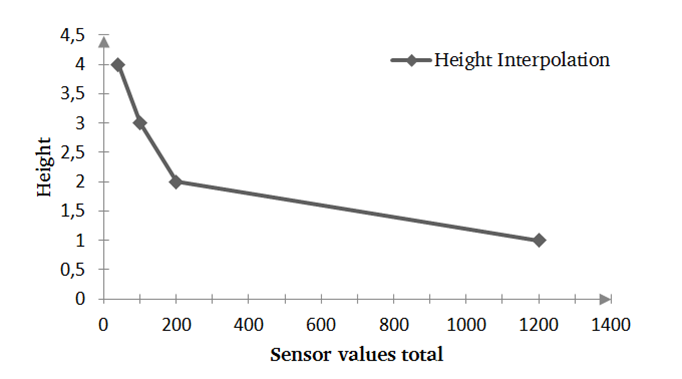
\includegraphics[width=0.6\textwidth]{images/magicbox_data_zaxis}
\caption{Piecewise linear hand distance estimation \cite{Braun2011MultiInputDevice}}
\label{fig:magicbox_data_zaxis}
\end{figure}
%Figure 29 Piecewise linear hand distance estimation [78]
The first data processing step of the MagicBox is the planar localization of the hand, following the weighted average algorithm previously presented. In order to calculate the distance of the hand from the plane we are using a piecewise linear interpolation, that resembles the response curve of a single sensor \cite{Braun2011MultiInputDevice}.
\begin{figure}[h]
\centering
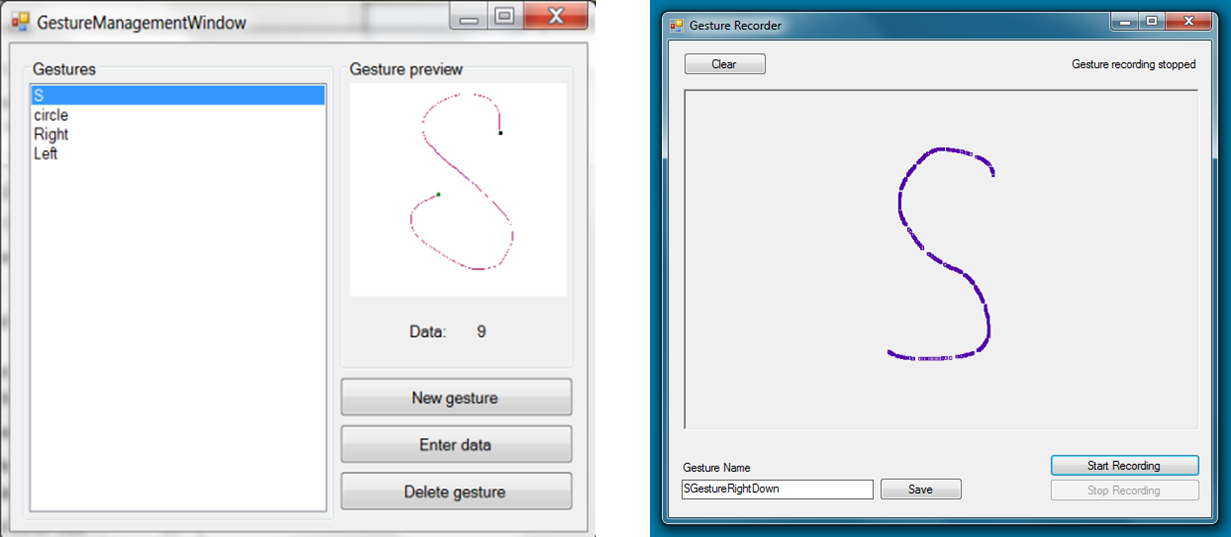
\includegraphics[width=0.7\textwidth]{images/magicbox_data_gest}
\caption{Gesture overview module (left) and gesture recorder (right)}
\label{fig:magicbox_data_gest}
\end{figure}
%Figure 30 Gesture overview module (left) and gesture recorder (right)
An addition of the MagicBox was a generic gesture recognition module based on methods similar to mouse gesture recognition \cite{braun2013capacitive}, albeit adapted for three dimensional locations. The developed debug software allows defining an arbitrary set of potential gestures and adding training data, as shown in Figure \ref{fig:magicbox_data_gest}. The module is looking for matches based on the most recent set of locations. 
\subsubsection{Large-area location tracking}
Using long wire electrodes may result in considerable noise and influence from outside electric fields. Therefore CapFloor requires preprocessing to reduce the noise and achieve a more robust high-level data processing. The localization uses the weighted average algorithm that has been presented previously. 
\begin{figure}[h]
\centering
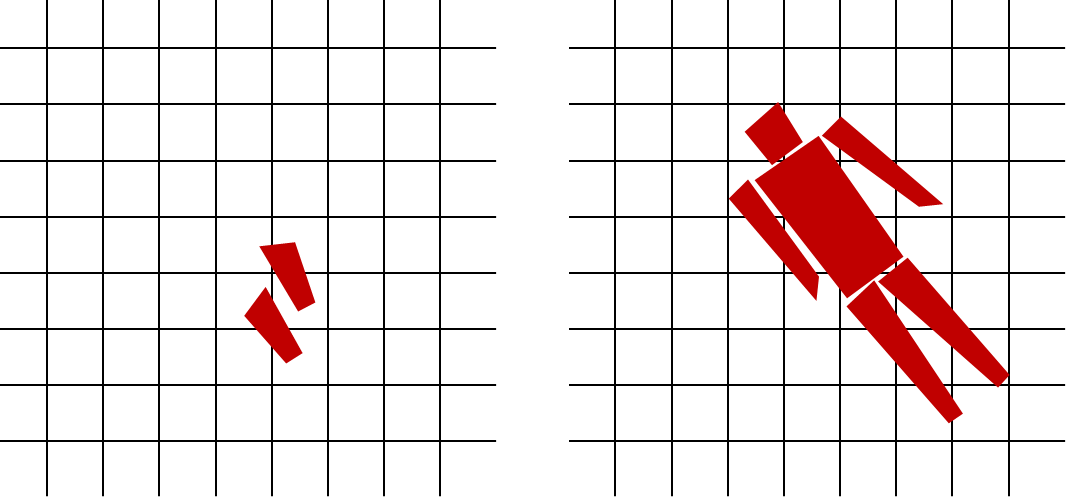
\includegraphics[width=0.8\textwidth]{images/floor_shapes}
\caption{Shapes of a standing and lynig person on top of the CapFloor grid}
\label{fig:capfloor_shapes}
\end{figure}
The fall detection is using a time-series analysis of the aggregated values of the sensors that are currently detecting an object. This method is using the assumption that the overall sensor response is roughly equivalent to the shape of the object that is closest to the surface, resulting in a higher capacitance of the overall system, similar to the plate capacitor model. This effect is shown in Figure \ref{fig:capfloor_shapes}. The sum $s$ of all n sensor values $r$ is the closest equivalent to the system capacitance and therefore a viable measure. If the overall value is beyond a certain threshold $v_l$ we can consider a lying person $p_l$.
\begin{equation}
s=\sum^n_{i=0}{r_i}\ \ \ ,\ \ \ p_l=\left\{ \begin{array}{c}
1,\ \ \ s\ge v_l \\ 
0,\ \ \ s<v_l \end{array}
\right.
\end{equation}
In order to increase the robustness this threshold has to be exceeded for a certain amount of time $t_m$. In consequence a fall $f$ is detected if the following equation is 1.
\begin{equation}
f=\prod^{t_m}_{j=0}{p_{l,t_j}}
\end{equation}
\subsection{Model-driven fitting methods}
\subsubsection{Single-body models}
\begin{figure}[h]
\centering
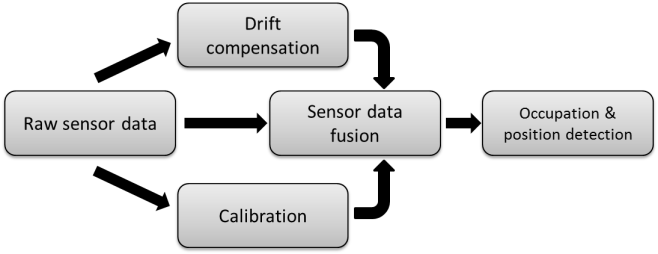
\includegraphics[width=0.7\textwidth]{images/smartbed_proc}
\caption{Data processing components \cite{braun2012context}}
\label{fig:smartbed_proc}
\end{figure}
The different components of the Smart Bed data processing are shown in Figure \ref{fig:smartbed_proc}. Raw sensor data is distributed to three different modules, the calibration which is determining the initial parameters for the sensor data fusion, the drift compensation that alters those parameters according to long term trends and finally the sensor data fusion module that processes the data and does feed it to the occupation \& position detection. Calibration and drift compensation follow the previously presented model \cite{braun2012context}. 
\begin{figure}[h]
\centering
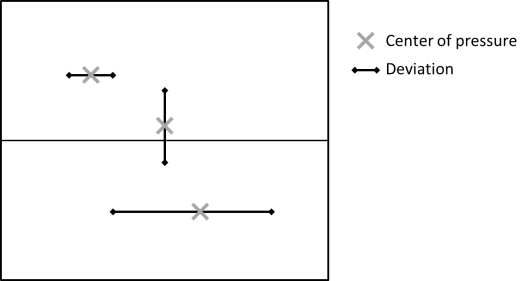
\includegraphics[width=0.7\textwidth]{images/smartbed_cog}
\caption{Calculating centers of pressures and deviation \cite{braun2012context}}
\label{fig:smartbed_cog}
\end{figure}
Occupation and position detection is performed by dividing the two person bed into left and right and individually calculating for each side the total sensor values, assumed center of pressure using weighted average and the standard deviation (Figure \ref{fig:smartbed_cog}). The same calculation is done between the two sides to distinguish where is activity or if one person is lying diagonally.
Using these six intermediate values we can now map various poses. If all activity is on one side and the horizontal deviation is low, we can assume that one person is sitting. We can additionally use the intermediate values to calculate more information, e.g. the exact location a person is sitting at. 
The data processing for the sleep phase recognition is based on detecting the sensor data variations in order to analyze movement. Discriminating between sleep phases using movement is a common approach that has been used in the past \cite{salmi86}. Using a sparse set of sensors it is possible to detect movement by comparing subsequent sensor readings and associate it to different sleep phases using different activity profiles. The system is based on the same prototype as the posture recognition system \cite{Djakow2013movibed}.
\subsubsection{Multi-body models}
\begin{figure}[h]
\centering
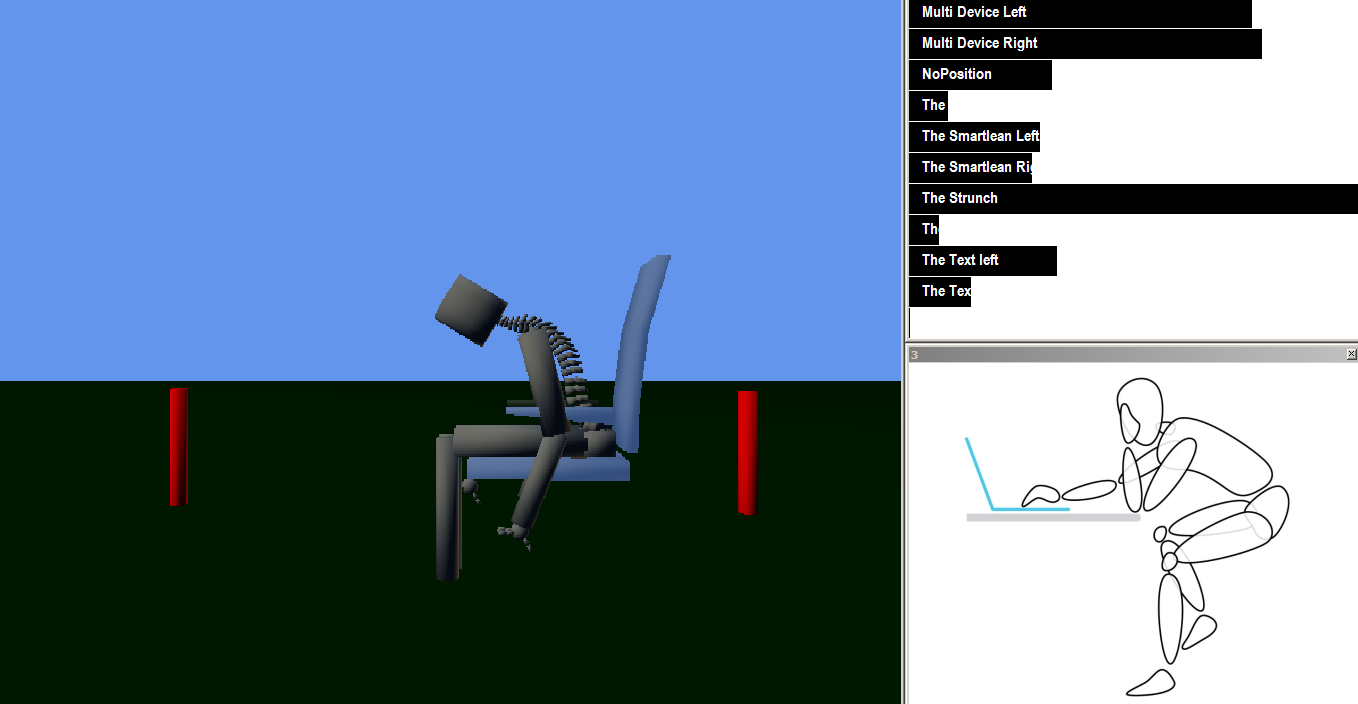
\includegraphics[width=0.7\textwidth]{images/smartchair_software}
\caption{Screenshot of the Capacitive Chair application showing the fitted 3D model on the left, posture detection on the upper right and the recognized posture on the lower right}
\label{fig:smartchair_software}
\end{figure}
In Figure \ref{fig:smartchair_software} we can see a screenshot of the Capacitive Chair debug application. On the left side we see a 3D model that is fitted to a chair model according to the current sensor values, in the middle the results of the machine learning module and the recognized posture and on the right side the currently running breathing rate detection as both Fourier analysis and signal deviation analysis.
All processing methods work on filtered and normalized sensor data. The difference in shape, material and size of the electrodes necessitates slight adaptations to noise filtering and data processing. As an example only the conductive thread backrest electrode is used in the breathing rate detection. 
The 3D model is using a simplified human joint model comprised of 13 connected components. Based on the current sensor readings, single parts or groups of components are fitted to the virtual chair. The process is a mix of posture mapping as found in the smart bed and modification of the dynamic links between the single components \cite{Braun2013ChairAid}.
\begin{figure}[h]
\centering
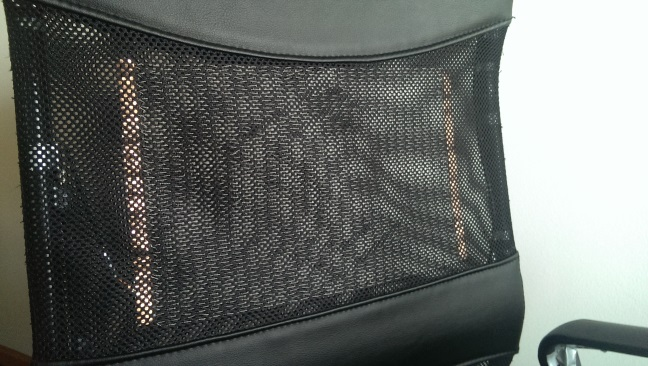
\includegraphics[width=0.7\textwidth]{images/smartchair_thread}
\caption{Screenshot of the Capacitive Chair application showing the fitted 3D model on the left, posture detection on the upper right and the recognized posture on the lower right}
\label{fig:smartchair_thread}
\end{figure}
We use a simple RBF neural network and training data collected by two different persons to match the input from eight sensors to nine potential output postures that are associated to different working situations. An early observation is that certain postures are difficult to distinguish given the limited number of sensors and the similarity of the postures on the rigid chair. Either a higher number of sensors or a more versatile chair could be used that allows gathering additional information required to distinguish the different poses more reliably. 

The breathing rate detection is operating on a single electrode that is integrated into a mesh on the backrest using conductive thread. The setup is shown in Figure \ref{fig:smartchair_thread}. Consequently the surface of the electrode is large and able to pick up the chest movement. Two different methods of data processing are used and fused to get the final breathing rate. Using a fast Fourier transformation the signal is transformed into the frequency space. We are looking for significant signal portions in frequency areas that can be associated to breathing, between $0.2Hz$ and $10Hz$. The second method is to look for zero-crossings of the sensor signal through an adaptive baseline. If a person is breathing in the sensor value will decrease resulting in the signal dropping below the long-term average, and rise above when the person is breathing out. Accordingly the breathing rate can be calculated by counting the zero-crossings.
\subsection{Heterogeneous sensor systems}
\subsubsection{Heterogeneous capacitive arrays}
\begin{figure}[h]
\centering
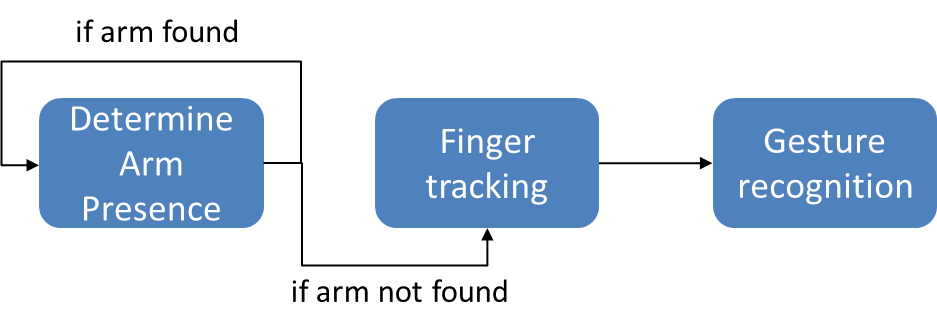
\includegraphics[width=0.4\textwidth]{images/armrest_dataproc}
\caption{Data processing pipeline of Active Armrest}
\label{fig:armrest_dataproc}
\end{figure}
%Figure 25 Data processing pipeline of Active Armrest
As we already mentioned, the Active Armrest electrodes are put into two groups. The data processing for both groups is distinctly different. In order to detect the presence of the arm using the two-electrode group a simple threshold on the accumulated values is used. The six sensor array in the front (touch area) is using the presented weighted average method to calculate finger positions. Additionally a threshold is used to distinguish one and two fingers. Overall there is a data processing pipeline as shown in Figure \ref{fig:armrest_proto}. The finger tracking and gesture recognition will be inactive until it is ensured that no arm is present. 

\subsubsection{Heterogeneous sensor fusion}
\begin{figure}[h]
\centering
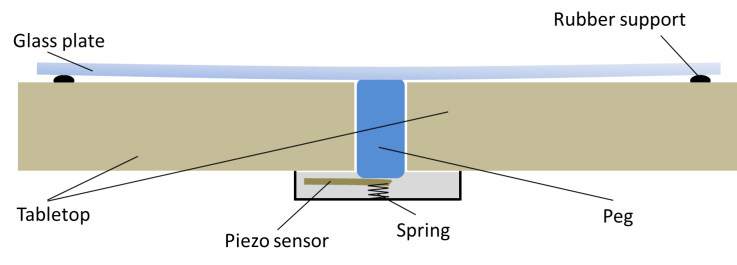
\includegraphics[width=0.7\textwidth]{images/captap_peg}
\caption{Suspended peg knock detection system for CapTap \cite{Braun2013ChairAid}}
\label{fig:captap_peg}
\end{figure}
%Figure 34 Suspended peg knock detection system for CapTap [80]
The hand location of the CapTap is similar to the methods presented for the MagicBox. We add the additional component of knock detection to provide selection events when touching the surface. Figure \ref{fig:captap_sketch} shows a sketch of the knock detection system. The table has a glass plate that is suspended on some rubber supports. In the center of the table we attach a small peg (enlarged in sketch) that creates a connection between the glass plate and a piezo sensor. If the glass plate starts vibrating from a touch we can measure this using the piezo sensor \cite{Braun2013ChairAid}. If a notable vibration is measured we are collecting the next 50 samples, resulting in a window of 250 milliseconds. To distinguish single and double knocks we calculate the weighted average within this window to get a measure for the distribution of sensor values within. If the average is closer to the beginning of the window the resulting event should be a single knock, and a double if the average is closer to the end of the window.
Hand localization and knock detection are working independently and are combined later in the software. It is reasonable to combine this, e.g. to ignore knock events that are occurring without a hand present. They may be indicative of a person doing a strong step close to the table.

\subsection{Image-based processing}
Their ability to detect changes in the electric field over a distance has led to capacitive proximity being regarded as similar to cameras. Smith et al. consequently called their approach electric field imaging, as particularly shunt mode measurements and their constrained electric fields allow applying certain image processing methods, e.g. tomography \cite{Smith1999a}. They were critical of using similar methods for shunt mode, noting the following statement.
\begin{quote}
Loading mode measurements can be likened
to images formed without a lens, since only one "end" of
each field line is constrained by the measurement. \cite{smith1998electric}
\end{quote}
Nonetheless, loading mode has certain advantages, particularly if all electrodes are in a single plane and we would like to have a higher sensitivity at a distance from the plane it is advantageous if there is no receiving potential nearby. One example for this planar electrode setup is large area gesture interaction devices, e.g. a table that is able to track the position of arms and hands in three dimensions. There is a plethora of image-based object detection and tracking algorithms that can be also used for capacitive proximity sensor data processing. There is a short process that I propose to realize this arm and hand tracking that includes some general steps that can be used to identify a variety of objects. The process is distinguished into four distinct steps:
\begin{itemize}
\item Creating a grayscale image from the acquired sensor data
\item Apply a feature-preserving image upscaling method
\item Find the contours of the present objects according to pixel values
\item Analyze the image moments of the contour areas and fit human arms
\end{itemize} 

\begin{figure}[h]
\centering

\includegraphics[width=0.5\textwidth]{images/proc_im_pixels}
\caption{Pixel array mapped from sensor values}
\label{fig:proc_im_pixels}
\end{figure}

The most challenging aspect of the first step is the low resolution of a reconstructed image. In order to achieve a mid-range distance resolution that allows detecting objects within 30 or 40 cm it is necessary to use electrodes that are sufficiently large. Thus, an example device uses an array of 6x4 sensor electrodes, resulting in an image of only 24 pixels. Typically the sensor values are an integer value in a range between 0 and 15000. Accordingly we can create a single-channel image with a channel depth of two bytes. In our case we use a linear mapping of sensor values to pixel intensities. An exemplary result image of this mapping is shown in \ref{fig:proc_im_pixels} (with enlarged pixels). In this format it is difficult to gather information about the exact position of the arms and thus we need to apply further processing before finding the contours and fitting arm objects.
\begin{figure}[h]
\centering
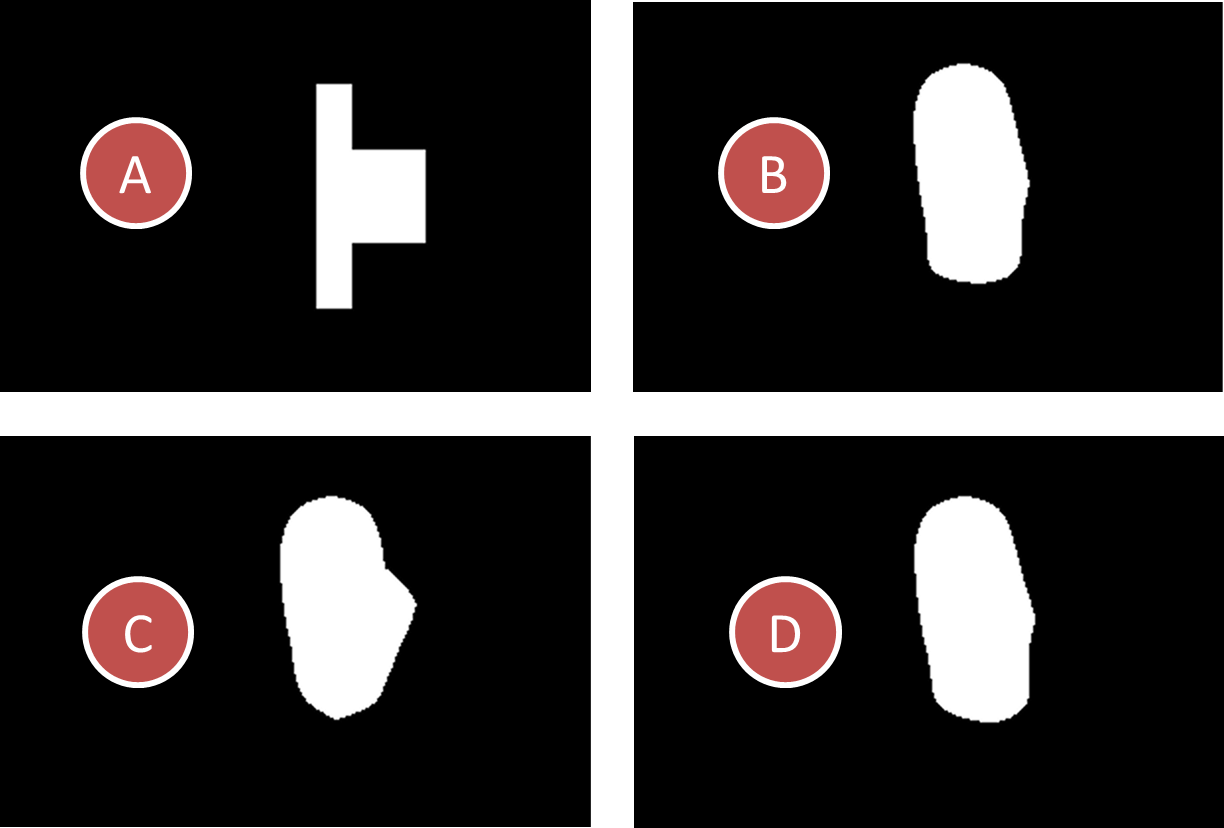
\includegraphics[width=0.9\textwidth]{images/proc_im_interpol}
\caption{Effect of different upscaling methods on shape, (A) nearest neighbor, (B) bicubic, (C) bilinear, (D) Lanczos4 - shown as thresholded binary images (pixel intensity > 30)}
\label{fig:proc_im_interpol}
\end{figure}

\subsubsection{Acquire and optimize contours}
In order to get the relevant contours of objects in the interaction area we have to apply some further processing. The first step is to enlarge the image using a feature-preserving scaling method. As all sensors are prone to environmental noise we apply some thresholding based on the pixel intensities before looking for contours. The result is an enlarged binary image of black and white pixels. We have tested four different image scaling methods, nearest neighbor, bilinear interpolation, bicubic interpolation and Lanczos interpolation. Exemplary results are shown in \ref{fig:proc_im_interpol}. The Lanczos interpolation showed the best results but is most processing intensive. However, since we are dealing with small images it is reasonable for CapTap. The contours are calculated based on those binary images, defined as the borders between black and white regions. For further processing we are looking into the distribution and the intensities of the pixels within the specified region.
\begin{figure}[h]
\centering
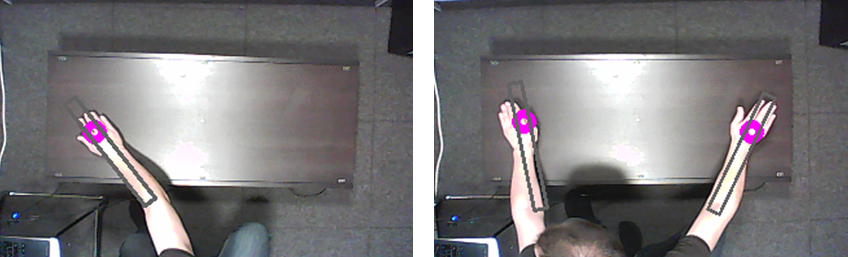
\includegraphics[width=0.9\textwidth]{images/proc_im_arms}
\caption{Overhead camera picture of the scene overlaid with live arm and palm reconstruction for one arm (left) and two arms (right)}
\label{fig:proc_im_arms}
\end{figure}

\subsubsection{Palm and arm fitting}
The last step of identifying and tracking the arms is to fit the position and orientation of the palms and arm into the acquired object contours. For this task we are analyzing the image moments within the contours. These are certain particular weighted averages of pixel intensities, or a function thereof \cite{hu1962visual}. They can be calculated using the following equation, whereas $j$ and $i$ define the order and $I(x,y)$ is the pixel intensity at a given position. We can use this to calculate the center point $(\overline{x},\overline{y})$, leading to the central moments $mu_ji$ that are required to determine the orientation of the contour as angle $\gamma$.
%m_ji=∑_(x,y)▒〖I(x,y) x^j y^i  〗,x ̅=m_10/m_00 ,y ̅=m_01/m_00 
%〖mu〗_ji=∑_(x,y)▒〖I(x,y) (x-x ̅ )^j (y-y ̅ )^i  〗
% γ=0.5∙arctan (2∙〖mu〗_11)/(〖mu〗_20-〖mu〗_02 )
\begin{equation}
m_ji=\sum_{(x,y)}{I(x,y)x^jy^i}
\end{equation}
\begin{equation}
\overline{x}=\frac{m_10}{m_00}, \overline{y}=\frac{m_01}{m_00}
\end{equation}
\begin{equation}
mu_{ji}=\sum_{(x,y)}{I(x,y)(x-\overline{x})^j(y-\overline{y})^i}
\end{equation}
\begin{equation}
\gamma=0.5\cdot arctan\frac{2\cdot{mu_{11}}}{mu_{20}-mu_{02}}
\end{equation}
 
We use the center point and orientation to calculate the estimated position of the palm of the hands. These points are the basis for the subsequent gesture recognition. Additionally, we are using separate Kalman filters for smoothing the different palm positions and arm orientation. The resulting arm reconstruction and the actual arm position in a photo are shown in \ref{fig:proc_im_arms}. We installed a simple webcam above the table and registered the table position to the camera image. 

The arm reconstruction so far is mostly used to determine the arm position. Another potential use of the arm orientation is to improve the merging of two hands. While the system can't distinguish from a single sensor if one hand is close or two hands are further away, we can use the presence of two arms to identify the overall number of objects in the detection range. 
\subsubsection{Intensity-based elevation estimate}
A distinct challenge of the capacitive hand tracking is the considerable directional difference in available resolution. While we can use the presented image analysis to track the planar position of the arms over the whole table area of 80cm width and 50cm depth, estimating the elevation of the arm above the table is restricted by the proximity range of the single sensor. Typically the achievable range maxes out at around 35cm, depending on environmental conditions. In a plate capacitor system the distance $d$ is proportional according to size of the plates $A$ and resulting capacitance $C$. Due to the linear mapping of sensor capacitance measurements to pixel intensities $I$ we can use the image moment within a contour $S$ as estimate of the actual capacitance, and calculate the elevation $e$ according to the following equations:

\begin{align}
d&\propto{\tfrac{C}{A}} & S&\propto{\tfrac{m_{00}}{\int{S}}}
\end{align}

The same thresholds discussed in the contour retrieval phase apply to this step, thus leading to discarding objects at a larger distance that are difficult to detect. Starting from this threshold we normalize the resulting elevation according to a maximum threshold for m00 that denotes a very close object (such as touch). The actual touch recognition is performed using acoustic methods. 
As previously explained the sensors are prone to environmental influences, thus this just allows to get an estimate of the actual elevation and no absolute distance value. Therefore, the interaction should not be designed to require a highly precise discrimination of different elevation values, but instead use more of a 2.5D paradigm. Our take on this will be presented in the application section.

\subsection{Physiological signals in frequency- and time-domain}

\clearpage
\section{Application prototypes}
% Table generated by Excel2LaTeX from sheet 'Tabelle2'
\begin{table}[htbp]
  \centering
  \footnotesize
  \caption{Overview of developed capacitive proximity sensing prototypes}
    \begin{tabularx}{\linewidth}{Xp{3.5cm}Xp{3.5cm}p{3.5cm}}
    \toprule
    \textbf{Name} & \textbf{Description} & \textbf{Application Areas} & \textbf{Measuring Layout} & \textbf{Data Processing} \\
    \midrule
    CapFloor & Capacitive system for indoor localization and fall detection based on electrode grid below the floor. & Indoor Localization & Loading mode, variable number of sensors based on area size & Binary activity association and using geometry for positioning. Monitoring of overall value for falls. \\
    Smart Bed & Capacitive sensors placed below mattress able to determine sleeping postures and breathing rate. & Smart Appliances, Physiological Sensing & Loading mode, four sensors on each side of bed  & Posture fitting using a static model. Fourier analysis for breathing rate recognition. \\
    The Capacitive Chair & Office chair equipped with capacitive sensors to distinguish different typical work postures and stress levels. & Smart Appliances, Physiological Sensing & Loading mode and shunt mode, eight sensors, heterogeneous sensing capabilities & Model fitting using a dynamic model. Fourier analysis for breathing rate detection. Posture recognition using machine learning. \\
    Active Armrest & Heterogeneous system for finger gesture recognition and arm rest identification for automotive applications. & Smart Appliances, Gestural Interaction & Loading mode, heterogeneous layout & Finger positioning using direct calculation. Binary arm presence detection. \\
    MagicBox & Mobile 3D gesture interaction device using an array of electrodes. & Gestural Interaction & Loading mode, six wireless sensor nodes & Geometric detection of hand relative to plane. Adapted mouse methods for gesture recognition. \\
    CapTap & Table capable of detecting 3D gestures and knocks to realize tactile interaction in a living room. & Smart Appliances, Gestural Interaction & Loading mode, 24 capacitive sensors and a single touch detecting microphone & Image-based hand and arm detection. Independent touch detection. Tracking of multiple objects. \\
    \bottomrule
    \end{tabularx}%
  \label{tab:prot_listown}%
\end{table}%

In the last few years I have created a number of different prototypes using capacitive proximity sensors in various usage scenarios within smart environments. They tackle specific application domains and implement one or more of the data processing methods that have been specified in the previous section. A short overview can be found in Table \ref{tab:prot_listown}. During the next few pages I will describe in detail how the prototypes have been created, how they implement the different data processing methods and outline the results of any technical evaluation and usability study that has been performed.
\subsection{CapFloor}
\begin{figure}[h]
\centering
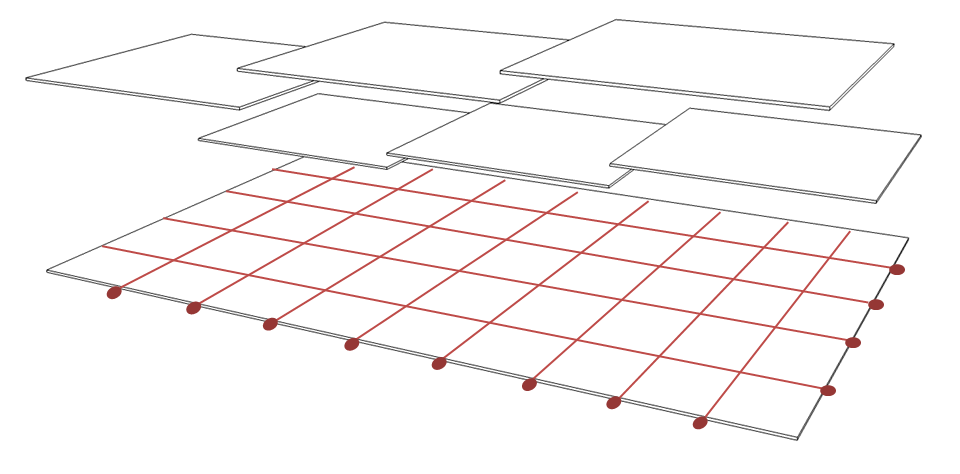
\includegraphics[width=0.8\textwidth]{images/capfloor}
\caption{CapFloor sketch - grid layout of electrodes is placed below a floor layer with sensors attached on the sides}
\label{fig:capfloor_sketch}
\end{figure}

CapFloor is a capacitive system for indoor localization and fall detection that is based on a grid array of sensing electrodes placed below a floor covering \cite{Braun2012CapFloor}. A sketch of the system is shown in Figure \ref{fig:capfloor_sketch}. The grid is comprised of insulated wires that are placed orthogonal to each other. Sensors are placed on two sides of the room. Each sensor is performing loading mode measurements. The system is intended to act as both indoor localization system and fall detector. CapFloor can be placed below any non-conductive material, like wood, tiles and PVC, if the distance between the wires and the floor surface is not too high. It can discriminate between a foot being above an electrode or a whole body. Combining this information from various sensors we are able to get a reliable detection of lying, sitting and standing persons. Using only two sides of the room for sensors it is possible to cut the wires without considerably affecting the signal; allowing easy installation in non-rectangular rooms.
Accordingly CapFloor is able to be used in various application scenarios. Indoor Localization in the home domain can be useful in energy saving and fall prevention by appropriately activating and deactivating the environment lighting. It can also be used in security-restricted areas to detect unauthorized movement. The fall detection should be used in a system that has various levels of escalation. E.g. it is not easy to distinguish between a person doing exercises on a floor and a person that has fallen down. Accordingly the system should query if the person is well and not autonomously call for outside help.

\subsubsection{Evaluation}
\begin{figure}[h]
\centering
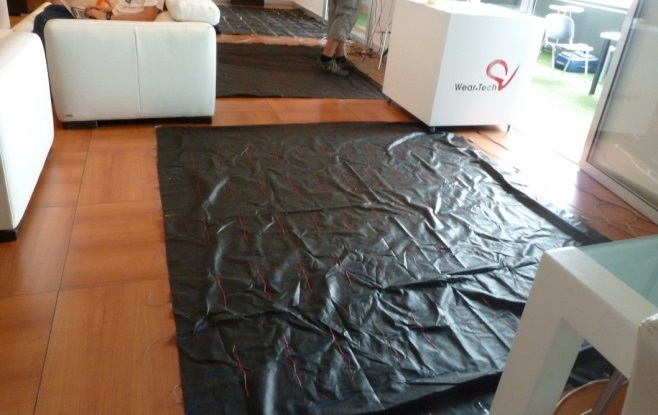
\includegraphics[width=0.8\textwidth]{images/capfloor_evaal}
\caption{Floor mats with integrated CapFloor system used at the EvAAL 2011 competition \cite{Braun2012CapFloor}}
\label{fig:capfloor_evaal}
\end{figure}
The CapFloor system was evaluated in the scope of the Indoor Localization Track of EvAAL 2011, where it participated out of competition \cite{chessa_eval}. In Figure \ref{fig:capfloor_evaal} we can see a picture of the demonstration setup installed in the living lap using the system integrated into different mats that are placed in the environment. The system was tuned to detect a single person and was able to perform this reasonably in the areas covered. The resolution of the system is strongly depending on the given density of electrode wires. While there is a certain measure of proximity, it is not possible to detect objects that are more than a few centimeters away from the wires. Later iterations of the system are using higher voltages and shunt mode measurements to improve the tracking reliability and enhance the fall detection.

\clearpage
\subsection{Smart Bed}
\begin{figure}[h]
\centering
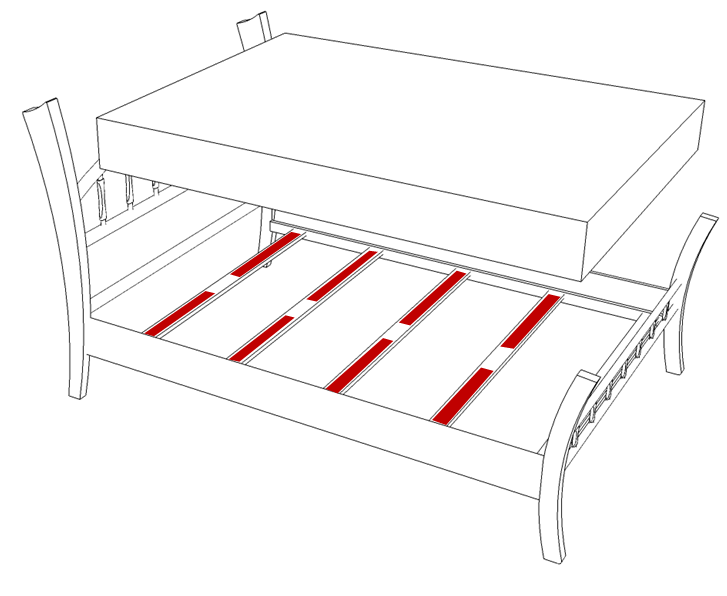
\includegraphics[width=0.7\textwidth]{images/smartbed}
\caption{Smart Bed sketch - flexible plate electrode are attached on spring board}
\label{fig:smartbed_sketch}
\end{figure}
The Smart Bed is a regular bed frame that has been equipped with capacitive proximity sensors in order to determine occupation, posture and sleep phases \cite{braun2012context}\cite{Djakow2013movibed}. A sketch can be seen in Figure \ref{fig:smartbed_sketch}.  The electrodes are comprised of copper foil that is attached to the flexible wooden panels of the slatted frame. This allows the electrodes to be sensitive to both proximity and applied pressure, resulting in a superposed combined sensor value that is considerably higher as opposed to proximity measure on its own. The electrodes are equally distributed, with four being on both sides of the two person bed. The system is able to determine different sitting and lying postures of one or two persons, including less regular lying positions such as diagonal or orthogonal to the long side of the bed. Using an analysis of the movement gathered by variation in the sensor signal the sleep phases can be analyzed, similar to accelerometer-based systems that are popular for smartphones \cite{krejcar2011}.

The Smart Bed can be used for various purposes. A main application is connecting the occupation detection to a home automation system and timer in order to activate ambient lighting if the person is get-ting up in the night, presumably to find the way to the restroom. Accordingly, in a single person household the lights in unoccupied rooms could be turned off in order to conserve energy. In the domain of personal health the Smart Bed is able to give the user a feedback on sleep quality based on the sleep phase measurement performed in the night. Another potential application is to use the acquired pressure distribution as indicator for back-friendly lying positions that may be harmful over a longer period of time \cite{Hamisu2010}.
The occupation and posture detection relies on a simplified body model to approximate the pressure distribution and sensor values to a certain posture \cite{braun2012context}.  

\begin{minipage}{\linewidth}
\centering
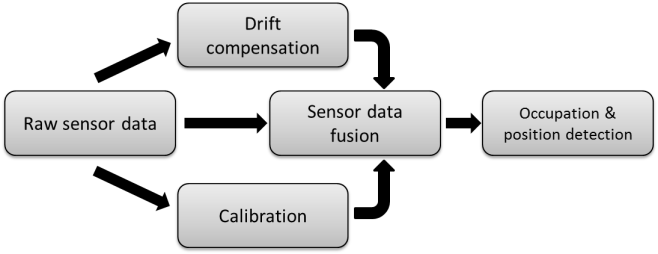
\includegraphics[width=0.7\textwidth]{images/smartbed_proc}
\captionof{figure}{Data processing components \cite{braun2012context}}
\label{fig:smartbed_proc}
\end{minipage}

The different components of the Smart Bed data processing are shown in Figure \ref{fig:smartbed_proc}. Raw sensor data is distributed to three different modules, the calibration which is determining the initial parameters for the sensor data fusion, the drift compensation that alters those parameters according to long term trends and finally the sensor data fusion module that processes the data and does feed it to the occupation \& position detection. Calibration and drift compensation follow the previously presented model \cite{braun2012context}. 

\begin{minipage}{\linewidth}
\centering
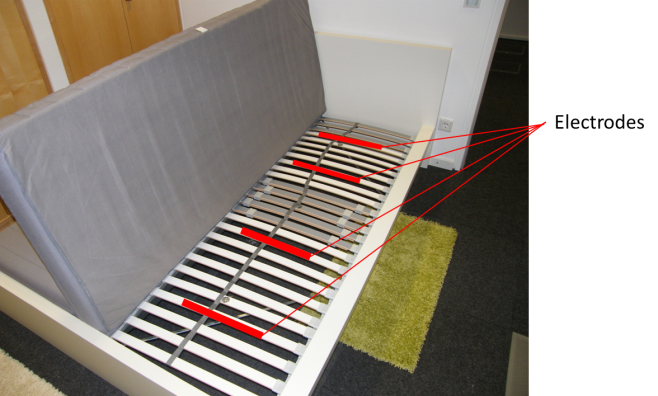
\includegraphics[width=0.8\textwidth]{images/disc_unob_bed}
\captionof{figure}{Electrodes and sensors hidden below mattress of Smart Bed \cite{braun2012context}}
\label{fig:disc_unob_elec}
\end{minipage}

The system prototype is shown in Figure \ref{fig:disc_unob_bed}. The positions of the electrodes on the slatted frame are indicated in red. The picture only shows one side of the bed. The same electrode positions are used on the other half of the bed.

The data processing for the sleep phase recognition is based on detecting the sensor data variations in order to analyze movement. Discriminating between sleep phases using movement is a common approach that has been used in the past \cite{salmi86}. Using a sparse set of sensors it is possible to detect movement by comparing subsequent sensor readings and associate it to different sleep phases using different activity profiles. The system is based on the same prototype as the posture recognition system \cite{Djakow2013movibed}.
 
\subsubsection{Evaluation}
\begin{figure}[h]
\centering
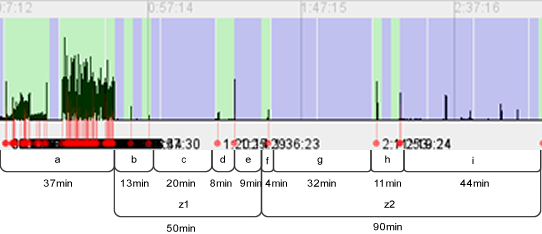
\includegraphics[width=0.9\textwidth]{images/smartbed_sleepphase}
\caption{Sleep movement data over three hours in one night \cite{Djakow2013movibed}}
\label{fig:smartbed_sleepphase}
\end{figure}
The Smart Bed posture recognition is able to successfully distinguish eight typical sitting and lying states. Using adaptation of the intermediate values it is possible to fit the state to an actual position on the bed, e.g. a \emph{person sitting on the right side of the bed} state can be modified to any location on that specific side of the bed. 
Regarding the detection of sleep phases there has been an evaluation and benchmarking of three nights \cite{Djakow2013movibed}. The Smart Bed was able to achieve a comparable performance to smartphone applications that detect sleep phases based on accelerometers. Figure \ref{fig:smartbed_sleepphase} gives an example of movement recordings using the capacitive proximity sensors over one night. The activities are grouped into distinct chunks that are later associated to the sleep phases. Currently breathing rate detection is added to the Smart Bed that can be used to improve the sleep phase detection and also can potentially detect anomalies that may be indicative of a certain health risk.

\clearpage
\subsection{The Capacitive Chair}
\begin{figure}[h]
\centering
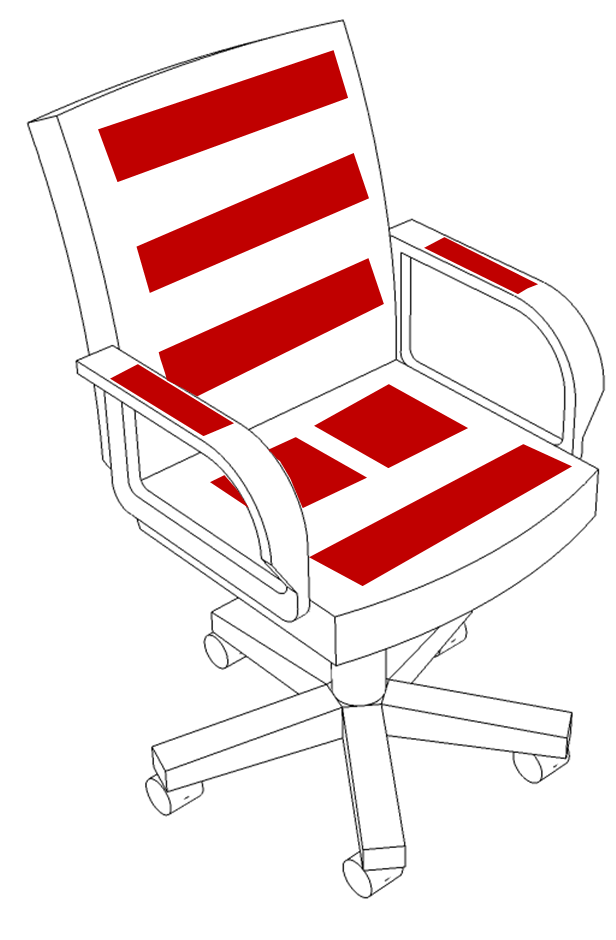
\includegraphics[width=0.4\textwidth]{images/smartofficechair}
\caption{Smart office chair sketch - eight electrodes three in backrest, three on seat and two in armrests}
\label{fig:smartchair_sketch}
\end{figure}
The Capacitive Chair is a regular office chair equipped with eight capacitive proximity sensors that can detect different sitting postures and work-related stress levels by examining movement and breathing rate \cite{Braun2013ChairAid}. Seven solid copper electrodes that are placed below the covering are augmented by a single conductive thread electrode that is placed in a mesh on the backrest. In the past smart chairs have used pressure sensors to infer posture and occupation \cite{tan2001sensing}. Combining presence and proximity sensing it is possible to directly infer postures where parts of the body do not touch the surface, e.g. if the body is arched towards the front, or if an arm is raised from the armrests. Additionally higher area electrodes in the backrest allow detecting the breathing rate by measuring the movement of the chest.

The Capacitive Chair aims at providing different services to a typical office worker and office managers. Using the occupation detection it is possible to advise for some type of physical activity, if the time spent in front of the screen was too long. The system can also advise the user to change to a more back-friendly posture or regularly switch the stance to achieve a more general workout. Using the breathing rate detection we are able to get some sort of measure of the current stress level associated to the given working situation. By adapting the environment it is possible to improve the working atmosphere and reduce stress. The Capacitive Chair uses a multifacetted data processing approach. A machine learning algorithm is associating the sensing data to one of nine different typical sitting positions, inspired by a recent study of sitting positions for modern device usage \cite{globalPosture}. An adaptive body model that is fitted to the current sensor values allows for fine grained adaptation of those postures. Finally a combination of Fourier and data variation analysis is calculating the current breathing rate \cite{Braun2013ChairAid}.

\subsubsection{Capacitive layout}
The Capacitive Chair is based on a single OpenCapSense board that supports eight different electrodes. In order to get the posture measurements we need to distribute the electrodes equally on the different areas of the seat. The measurement of the breathing rate requires a larger electrode near the chest area. Consequently the electrodes are placed as follows:
\begin{enumerate}
\item Electrode on the upper part of the backrest (covered by faux leather)
\item Electrode in the central part of the backrest (using conductive thread)
\item Electrode in the lower part of the backrest (covered by faux leather)
\item Electrode below the right armrest
\item Electrode below the left armrest
\item Electrode for the left hip area below the left part of the seat
\item Electrode for the right hip area below the right part of the seat
\item Electrode for detecting both legs below the front part of the seat
\end{enumerate}

\begin{minipage}{\linewidth}
\centering
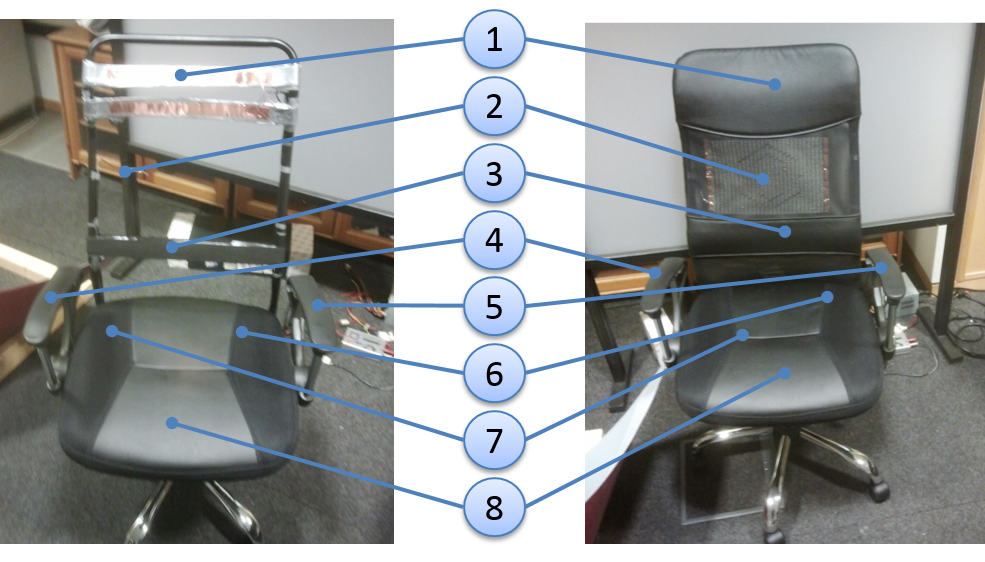
\includegraphics[width=0.8\textwidth]{images/prot_capchair_electrode_layout}
\captionof{figure}{Capacitive Chair electrode positions}
\label{fig:prot_capchair_electrode_layout}
\end{minipage}

The electrode is connected to channel 0 (CH0) of the OpenCapSense evaluation board. The following figure shows the layout of the electrode (2) including sensing electronics (5). The shield electrode is additionally the support structure for the whole setup here. The shield electrode is comprised of copper sheet bedded in duct tape. On the duct tape there are strips of copper sheet applied using conductive glue (2). The copper sheet is the sensing electrode connected to the sensor (5) using the blue wire (4). The shield electrode is connected using the red wire. The frame of the backrest is indicated using the number (6). 
This electrode in the lower part of the backrest is connected to CH2 of the OpenCapSense evaluation board.
The layout is analog to the one on the upper part of the backrest, comprised of shield electrode (2) covered by duct tape and a copper sheet electrode. The electrode on the right armrest is connected to CH3, the one on the left side to CH4 of the OpenCapSense evaluation board. Both electrodes are comprised of a copper sheet fixed to the armrest using duct tape. 
The electrode below the right hip area is connected to CH5, the one below the left hip area to CH6 and the leg electrode to CH7.
The figure above shows the electrodes. All of them are made of unprocessed, two-layer copper PCBs. They are isolated to the environment using duct tape. The electrode for the leg area is comprised of two distinct PCBs (2,3) that are connected using copper wire (5). The hip electrodes (1) are similarly comprised of copper PCBs. The wires are guided through the wooden seat using small drill holes (4,6). The red wire leads to the sensing electrode while the grey wire leads to the shielding.

\begin{minipage}{\linewidth}
\centering
\includegraphics[width=0.8\textwidth]{images/prot_capchair_threadelectrode}
\captionof{figure}{Detail view of conductive thread electrode}
\label{fig:prot_capchair_threadelectrode}
\end{minipage}

The electrode in the central part of the backrest is connected to CH1 of the OpenCapsense evaluation board.
The electrode (1) is comprised of conductive thread that was woven into the covering of the backrest. The ends of the conductive thread are connected to a conductive copper foil. This foil is formed in such a way (4 left) that a terminal (4 right) can be applied and connected to the sensor electronics (3). This type of electrode does not support any shielding. In order to remove the covering the terminal should be disconnected from the electrode first.
 
\subsubsection{Processing}
The first step of data processing is filtering. We have implemented different types of filters, including static average and floating average filters. In this case we are using a median filter that is taking the median value of eight previous samples. After filtering we are building the baseline for each sensor channel. The baseline is the minimal sensor value that is created by sampling the environment without any object present. There is a plausibility check in this step to discard values that deviate too far from the norm. The maximum values of a channel are collected on run-time. Again we are using a plausibility check. The final step of pre-processing is a normalization based on acquired minimum and maximum values. For further processing we additionally need information about short-term value variance that we gather by calculating the difference quotient using a sample of ten average filtered measurements.
Afterwards we are performing a fast fourier transformation (FFT) to get information about the frequency spectrum of the sensor values, in order to perform breathing rate detection. 
\subsubsection*{Breathing rate detection} 
We are using the FFT values of sensors attached to the central backrest to get the current breathing rate. A binning operation is performed to look for significant signals in a reasonable frequency interval (0.1Hz-3Hz).
In order to increase the reliability of the breathing rate detection we use a second method. Based on the normalized values a mean value curve is calculated. The intersection points of this mean value curve and the current sensor values are additionally stored. We are using a dynamically weighted combination of both values to increase the reliability of the breathing rate detection.
\subsubsection*{Posture recognition, kinematics of the human body}
The processed values of all sensors are compared to previously trained sitting positions of a user. The position with the lowest deviation is considered the current posture. Currently the system supports nine different postures; however it can be dynamically extended or reduced.
Based on the normalized sensor values and geometric positions of the sensors the data is interpreted as position of the different joints of a user. 
4.2.4	Output
The GUI allows displaying of raw and processed data. In the following section we are presenting the different forms of interaction.
 
Figure 13 GUI with four opened windows
Figure 11 gives on overview of the GUI. Selecting the desired output in the ToolBox (1) opens the associated window. In this case we can see the data display of sensor channel 1 (2), the recognized breathing rate (4), the FFT of sensor channel 1 (3) and the recognized postures and their deviations (5).
 
Figure 14 GUI with two windows
Figure 12 shows two additional windows. On the left side (1) we can see a picture depicting the currently recognized posture; on the right side (2) we can see the human model with recognized joint positions. The 3D joint recognition is still in strong development and will be remodeled in the future.
Additional screens that have not been shown in this overview are a serial monitor that displays the raw data acquired from the USB connection, the collection of measurements using software queries, the display of all sensor values in table format and a repositioning of the different windows.
\subsubsection*{Distinguish work activity levels}
 
Figure 15 Work Activity aggregation over a single work day (mock-up)
Figure 13 shows a mock-up of a typical work day activity over a single work day. We assume the work day of a typical office worker and support three different aggregated activities: 
Active work as indicated by a certain level of movement while on the chair
Passive work as being present on the chair while not moving a lot
Not present at desk, whereas no one is currently sitting on the chair.


\subsubsection{Evaluation}
The Capacitive Chair was partially supported by the EIT ICT Labs project Cognitive Endurance during 2013. In this scope it was evaluated in two distinct studies. The first aimed at testing the aggregated recognition of working activities with several persons over various days. The second study was testing the posture recognition with various users that were additionally queried about their general impression of the system. In this section we are presenting results of both studies.
\subsubsection*{Working situation recognition}
The sensing chair supports distinguishing two different working situations that are determined using the method described in the previous section. The system also supports sending to the Cognitive Endurance server.
 
Figure \ref{fig:prot_capchair_eval_work} shows an example of this generated activity log. We have performed a test over 3 days between December 4th 2013 and December 6th 2013 on a typical work day in the office. The resulting activity logs were used to generate a chart as shown in the previous section. An example chart is shown in Figure 15.

\begin{minipage}{\linewidth}
\centering
\includegraphics[width=0.8\textwidth]{images/prot_capchair_eval_work}
\captionof{figure}{Example chart of work activity data collected}
\label{fig:prot_capchair_eval_work}
\end{minipage}	

We can clearly see some phases of not at chair - usually for lunch break or some meetings and the work is distributed between active work, such as writing and typing and longer phases of inactivity (such as reading).

\subsubsection*{Posture recognition - test 1}
In a second evaluation we were testing the posture recognition of the chair in a short study with 10 participants. Our system was tuned to distinguish three poses and a non-pose:
\begin{itemize}
\item Sitting upright
\item Sitting hunched
\item “Slouching on chair”
\item Close to chair - disturber
\end{itemize}

The persons were given a short introduction, the different postures were displayed, and finally the persons were asked to perform the postures in order. When testing “close-to-chair” the subjects were asked to rattle at the chair, stand close, move it around and thus disturb the potential sensor readings. Each class was tested for 10 seconds, collecting 200 samples. Some impressions can be found in the following pictures:

\begin{minipage}{\linewidth}
\centering
\includegraphics[width=0.8\textwidth]{images/prot_capchair_eval_pos1}
\captionof{figure}{Disturber position of a participant (left) and sitting upright (right)}
\label{fig:prot_capchair_eval_pos1}
\end{minipage}	 

\begin{minipage}{\linewidth}
\centering
\includegraphics[width=0.8\textwidth]{images/prot_capchair_eval_pos2}
\captionof{figure}{Slouching position (left) and sitting hunched (right)}
\label{fig:prot_capchair_eval_pos2}
\end{minipage}

Overall the results were very convincing. Of the 40 different measurements series only two were not achieving 100\% accuracy. The Upright and Disturbance positions were classified correctly for all candidates. A single candidate had an 86\% rating on the hunched posture. A different candidate had a 55\% rating on the slouching position. The average of correctly classified postures is 98,5\%.



\clearpage
\subsection{Active Armrest}
\label{ch:prot_armrest}
\begin{figure}[ht]
\centering
\includegraphics[width=0.4\textwidth]{images/active_armrest}
\caption{Active armrest sketch - six electrodes for finger gesture detection in front, two for arm detection in back}
\label{fig:armrest_sketch}
\end{figure}

Touch screens are by now also a trend in vehicles, with touch screens and touch pads becoming more common. The Tesla Model S provides a large area touch screen that completely replaces conventional button-based interfaces.  However, touchscreens have been identified as potentially distracting for the driver \cite{rumelin2013make}. My idea was to create a gesture input device based on capacitive proximity sensors, and unobtrusively integrate it into the car interior \cite{braun2013ActiveArmrest}. A suitable area for creating an interactive zone is the armrest, as it is the intended resting position in the first place. However, this creates an additional challenge. As the majority of interactions between arm and armrest are not intended to control aspects of the car system, we need concepts to infer the intention of the driver to interact with the car. The method has been described previously in Section \ref{ch:proc_hetero}. A sketch of this concept is shown in Figure \ref{fig:armrest_sketch}. To test the validity of the invisible interactive areas and the two interaction concepts, we have created the Active Armrest, a prototype comprised of an aftermarket armrest with an integrated heterogeneous array of eight capacitive proximity sensors - two using large electrodes for detecting arm proximity and orientation and six using small electrodes to create an interaction area in front of the armrest. The system uses the classification method described in Section \ref{ch:proc_hetero}.

\begin{figure}[ht]
\centering
\includegraphics[width=0.8\textwidth]{images/armrest_proto}
\caption{Active Armrest prototype, left - outside view, right - detail view of electronics \cite{braun2013ActiveArmrest}.}
\label{fig:armrest_proto}
\end{figure}

In order to evaluate the Active Armrest we have built the prototype shown in Figure \ref{fig:armrest_proto}. An aftermarket armrest was equipped with an OpenCapSense toolkit. The kit had to be modified due to the constrained interior and uses fixed wiring instead of USB connections. The demonstration application is based on the SenseKit debug software supplied with the toolkit. As of now there is a simple USB connection to a nearby PC. The gesture recognition framework was implemented in Java using the WEKA machine learning framework for SVM classification. A car interior demonstration application was created using Java and the Swing framework and mimics typical menu systems found on a touch screen.

\begin{figure}[ht]
\centering
\includegraphics[width=0.8\textwidth]{images/armrest_postures}
\caption{Postures of limbs on armrest - resting position (left),  arm raised position (middle), hand raised position (right) \cite{braun2013ActiveArmrest}.}
\label{fig:armrest_postures}
\end{figure}

In Figure \ref{fig:armrest_postures} we can see the three different positions arm and hand can have on the armrest. On the left, arm and hand are in resting position with both close to the surface. The middle image shows the arm raised position and fingers touching the front of the armrest. The right picture shows the arm resting on the back and the hand in proximity of the front area. The system is able to distinguish between the three different positions using the methods presented in Section \ref{ch:proc_hetero}. A set of four different gestures has been defined for both interaction methods. The number is sufficient to control the user interface that was developed and supports both navigation and selection. The type of gestures has been defined after looking at previous research into touch and hand gestures \cite{bragdon2011experimental, wachs2011vision}. For the touch interaction, left and right swipes performed with either one or multiple fingers are supported. Regarding the free-air interaction we are using left and right swipes, as well as planar circles either clockwise or counter-clockwise.

\begin{figure}[ht]
\centering
\includegraphics[width=0.8\textwidth]{images/armrest_demo_app}
\caption{Active Armrest demo software, left - finger tracker, right - OSM based navigation application \cite{braun2013ActiveArmrest}}
\label{fig:armrest_demo_app}
\end{figure}

Figure \ref{fig:armrest_demo_app} shows two screenshots of the created demonstration application. It allows to control radio stations, selecting different audio files and looking at images. It is controlled using the gesture sets explained above. The applications use a Next/Previous pattern for navigation within a UI level and Select/Back gestures to switch between the different levels of the UI.

\subsubsection{Evaluation}
\begin{figure}[ht]
\centering
\includegraphics[width=0.8\textwidth]{images/armrest_eval_confustion}
\caption{Confusion matrices of recognized gestures for touch interaction (left) and free-air interaction (right)}
\label{fig:armrest_eval_confustion}
\end{figure}

We performed a study with 11 participants investigating three different aspects - the detection rate of the gesture recognition system, differences in interaction speed between the two methods and getting a general feedback on the usability of our system. After a short introduction, the participants were asked to perform each gesture 4 times for both sets in alternating starting order. The results are shown in Figure \ref{fig:armrest_eval_confustion}. The touch interaction performed reasonably with a detection rate between $79.5\%$ and $90.9\%$ for each gesture. The detection rates of the free-air interaction were considerably lower, ranging from $45.5\%$ for counter-clockwise circles to $81.8\%$ for swipes to the right. The main issue is distinguishing between single and multi-touches. A personalized threshold that is calibrated to the user might alleviate this issue in future iterations. The interaction zone above the finger area is limited to a range of about 15 cm. While performing the circular gestures the participants often left this area, leading to misattribution to swipe gestures.

In the second part of the evaluation the participants had to perform a task in the presented demonstration application - selecting and playing back a certain music file. We calculated the time required to perform the task. The average time for free-air gestures ($\mu=125.67s, \sigma=95.12s$) was considerably higher than the average task completion time for touch gestures ($\mu=34.26s, \sigma=28.61s$). It is noticeable that there is a very high deviation of the different runs, while the touch gestures fare better in general. While many users were able to quickly perform the task, others had a high number of errors and required several minutes. We can assume that a certain amount of training can reduce the required time. A trained user not participating in the study required 11 s for the touch gestures and 18 s for the free air gestures.

Finally, we asked the participants to fill a general questionnaire on their experience with the Active Armrest comprised of a number of Likert-scale (1-10) questions. There was a strong preference for the touch gestures, in line with the results of the interaction time and gesture recognition study (1=touch gestures, $\mu=1.72, \sigma=0.84$). Most participants could imagine using the system for a longer period of time in their cars (10=strong agree, $\mu=8.00, \sigma=2.00$) and considered the device intuitive to use (10=strong agree, $\mu=8.36, \sigma=1.67$) and is an interesting interaction device (10=strong agree, $\mu=8.63, \sigma=1.26$). The touch interaction pattern was considered easier to use (10=very easy, $\mu=8.00, \sigma=2.45$) than the free-air interaction (10=very easy, $\mu=3.64, \sigma=2.68$). The opinions on the device precision were mixed (10=very precise $\mu=7.27, \sigma=2.43$).


\clearpage
\subsection{Magic Box}
\begin{figure}[h]
\centering
\includegraphics[width=0.6\textwidth]{images/magicbox}
\caption{MagicBox sketch - six electrodes uniformly distributed below surface}
\label{fig:magicbox_sketch}
\end{figure}
%Figure 28 MagicBox sketch - six electrodes uniformly distributed below surface
The so-called MagicBox was our first attempt to create an interaction device based on capacitive proximity sensing. It is using an array of six individual wireless capacitive sensors that communicate to a central station \cite{Braun2011MultiInputDevice}. The electrodes are using a large surface area and are made of aluminum foil. A sketch is shown in Figure \ref{fig:magicbox_sketch}. The system is able to track the position of a single hand in three dimensions up to a distance of approximately $20cm$, and uses different methods to infer gestures from the hand movement. 
It is designed to be a generic interaction device that can potentially be hidden below non-conductive surfaces. As it can be used without touching it is also applicable in sterile environments. A suite of demonstration applications has been created that showcase typical scenarios for the MagicBox. This includes multimedia applications, like image viewer and media player but also a 3D object viewer intended as demonstrator for potential medical applications, allowing a surgeon to check MRT or CT images in a sterile environment without touching any surface.

\subsubsection{Evaluation}
\begin{figure}[h]
\centering
\includegraphics[width=0.8\textwidth]{images/magicbox_proto}
\caption{MagicBox conceptual rendering (left) and detail view of electronics (right) \cite{Braun2011MultiInputDevice}}
\label{fig:magicbox_proto}
\end{figure}
%Figure 31 MagicBox conceptual rendering (left) and detail view of electronics (right) [78]
The MagicBox prototype is based on the Cypress First Touch starter kit \cite{cypressfirst} and combines six capaci-tive sensors communicating wirelessly to a single base station, that are put together with a USB-rechargeable power supply into a casing. A concep-tual rendering showing the interaction area and a detail view of the prototype electronics are shown in Figure \ref{fig:magicbox_proto}.
\begin{figure}[h]
\centering
\includegraphics[width=0.8\textwidth]{images/magicbox_eval}
\caption{MagicBox demonstration application - 3D object viewer (left) and image viewer (right) \cite{Braun2011MultiInputDevice}}
\label{fig:magicbox_eval}
\end{figure}
%Figure 32 MagicBox demonstration application - 3D object viewer (left) and image viewer (right) [78]
The different iterations of the MagicBox have been evaluated in conjunction with various demon-stration applications. A usability study with 18 per-sons led to general approval of the system \cite{Braun2011MultiInputDevice}. Two of the applications used in this study are shown in Figure \ref{fig:magicbox_eval}. On the left is a 3D object viewer that has to be controlled by a combination of menu and direct manipulation of the screen content. On the right side there is an image viewer that was controlled by gesture to trigger the next/previous images or perform zooming operations. The most common positive remarks gathered in this study can be roughly put into three groups:
\begin{itemize}
\item{The device very intuitive to use}
\item{The idea of interacting this way is novel and interesting}
\item{It is easy to control applications with those gestures}
\end{itemize}
Likewise we identified three main groups for negative comments about the prototype:
\begin{itemize}
\item{The device is not very precise}
\item{The interaction speed is slow}
\item{It can be tiring for the arm}
\end{itemize}
Later iterations have been trying to improve some of the weaknesses presented above, e.g. by using a more sophisticated gesture recognition system and faster sensor refresh rates. Accordingly there were fewer complaints about interaction speed and precision \cite{braun2013capacitive}. However, the final complaint about the device being tiring for the arm, requires a different approach, that we are investigating in the final prototype to be presented in this system.

\clearpage
\subsection{CapTap}
\begin{figure}[h]
\centering
\includegraphics[width=0.7\textwidth]{images/captap_v2}
\caption{CapTap sketch - 24 electrodes placed under table surface and a single detector for touch events}
\label{fig:captap_sketch}
\end{figure}
A general insight of free-air gestural interaction that became apparent even in early works is the physical demands of prolonged interaction with such systems \cite{Baudel1993, lenman2002} and the difficulty to adapt selection events to gestural input - the latter typically being realized by time- or position-based gestures \cite{Baudel1993,Krum2002}. There is no trivial solution to this challenge and any approach has to take into account the specific application scenario covered. Some systems attempt to provide specifically adapted graphical interfaces, while others include additional input devices assisting the interaction \cite{Wu2003,zimmerman1987hand}. A major point is decreasing the required time for interaction, e.g. by adding a tactile feedback to the interaction system, preventing time-based selection gestures. CapTap is a regular living room table that includes a capacitive proximity sensor array for tracking the position of one or more arms. As it is difficult for this sensor category to detect touch, if the interaction surface is at a distance from the electrodes, a hidden acoustic system is added that allows recognizing different touch events. CapTap tracks hand and arm position using the image-based object recognition previously presented and fuses this data with different touch events generated by a single contact microphone that analyzes the audio signals in frequency space. This allows to significantly reduce interaction time, as opposed to systems relying on time-based dwell gestures. The system was created in 2013 and 2014 with collaboration of several students, most notably Sebastian Zander-Walz and Stefan Frank \cite{Braun2013captap}. It is used and further developed within the European research project POSEIDON that aims at providing technical solutions to help persons with Down's syndrome on planning their day, as input device that allows interaction regardless of motoric skill level.
\subsubsection{Capacitive layout}
\begin{minipage}{\linewidth}
\centering
\includegraphics[width=0.8\textwidth]{images/prototype_views_new}
\captionof{figure}{Detail views of the prototype system: left - electrodes and sensors, right - audio interface and contact microphone}
\label{fig:prototype_views_new}
\end{minipage}	
 
Our goal with CapTap is to enable tracking of hands and arms that move above a table. Therefore, the electrodes are placed in an uniform array that provides similar sensing properties for the whole surface. It is realized as a prototype installed in a regular living room table. It is comprised of an array of capacitive proximity sensors, a contact microphone for touch event detection and a miniature PC. All devices can be integrated into the table in a way that it is not distinguishable from the not-augmented piece of furniture. Figure \ref{fig:prototype_views_new} shows some detail views of the disassembled prototype. The left image shows the back of the wooden tabletop. The electrodes are arranged in a 6x4 array and each one is attached to a single sensor. The right picture shows the touch detection microphone. It is attached in the center of the surface, as to avoid non-uniform sound distribution over the surface area that would be more difficult to train. Placing the microphone below the surface has no strong influence. However, a specific training phase is required for any novel surface that is equipped with the touch detection devices. 

\begin{minipage}{\linewidth}
\centering
\includegraphics[width=0.8\textwidth]{images/captap_schematics}
\captionof{figure}{Abstract view below the surface of the prototype including capacitive sensing electrodes and touch detection microphone}
\label{fig:captap_schematics}
\end{minipage}

The setup is visualized in Figure \ref{fig:captap_schematics}. The system is comprised of 24 electrode \& sensor pairs that are connected to three different measurement boards. The microphone is attached to a USB Audio Interface. Overall there are four different boards connected via USB to a  PC that executes and merges the different types of data processing and links it to the software suite. The prototype is based on OpenCapSense, a more advanced prototyping system presented by Grosse-Puppendahl et al. \cite{grosse2013opencapsense}. The boards are performing some prefiltering, whereas the image-based hand tracking is realized on an attached PC. The microphone is attached to an USB audio interface (M-Audio M-Track Quad) that transfers data acquired by up to four microphones and provides various pre-sampling functions. All four devices are attached to a Mini-PC that is performing subsequent data processing and is running the demonstration and testing applications. 
 
\begin{minipage}{\linewidth}
\centering
\includegraphics[width=0.8\textwidth]{images/table_final_view}
\captionof{figure}{Views of final prototype, complete view (left), top view with markers for touch evaluation (right)}
\label{fig:table_final_view}
\end{minipage}

The final table prototype can be seen in Figure \ref{fig:table_final_view}. On the left side the table is seen without any additional markers - on the right side we see the table equipped for the evaluation using a set of markers for different touch and swipe events. The debug software was developed with C\# using the .NET 4.5 framework. We are using the Emgu CV library based on OpenCV for image processing and application of the Kalman filter to the determined palm locations. The sound processing is implemented in C++ and Java using a modified version of ChucK for audio sampling and the WEKA framework to apply the machine learning on top. We are using sockets to transfer data between the different modules. The debug application allows a fine control of the various processing steps in both image and audio signal processing.

%\begin{minipage}{\linewidth}
%\centering
%\includegraphics[width=1.0\textwidth]{images/alltouch}
%\captionof{figure}{64 sample FFTs and photo for a knock event (A), a finger tap (B), a finger swipe (C) and a hand swipe (D)}
%\label{fig:alltouch}
%\end{minipage}

\subsubsection{Processing}
CapTap is using the image-based algorithm for tracking palms and arms that was presented in the processing section. An addition is the touch recognition based on acoustic tracking. The method was inspired by the works of Harrison et al. \cite{harrison2011tapsense} with various modifications to allow identifying both impact and swipe events. At first the audio signal is acquired using a 96kHz sample rate and a feature extraction rate of 375Hz (using a  Hanning type sliding window of 4096 (and 256 samples overlapping) samples per extraction. In order to perform a classification over this signal we have to look at a variety of different features.
\subsubsection*{Feature vector}
The signal differences are most significant in the frequency domain, thus we are performing a FFT over 4096 samples, looking at the first 512 of 2048 magnitude values, thus covering the frequency range up to 12kHz. We are collecting the mean value, the standard deviation and the index of the highest value within the frequency range. This process is repeated for a downsampled FFT of 64 values, similar to the method used by Harrison et al. Another frequency domain-feature we are using is the centroid, i.e. the weighted mean of the present frequencies. Additionally, we are using two time-domain features, the RMS power (root mean square), i.e. the average magnitude within the current frequency band and the number of zero crossings of the signal. 
\subsubsection*{Classification}
We have to distinguish two different classifiers that are used for impact and swiping events. Even though knocks and taps are temporal gestures they are short in duration, while the swipe gestures are constant for a longer time period. Example 64-value FFTs are shown in Figure \ref{fig:alltouch}, with impact events and their low-frequency peaks on the left and swipe events and their fairly constant value on the right. For impact events we are using some metrics to identify the point at which the features shall be analyzed. A simple preprocessing identifies increasing power in lower frequencies and begins to store all feature vectors until a maximum is reached or the power is decreasing again. Not relevant secondary power increases (that are prevalent on stronger knocking events) are ignored. The feature vector corresponding to the maximum is then put into the classifier. This is a trained SMO classifier comprised of a support vector machine and a polynomial kernel that matches five different impacts - single knock, double knock, single finger tap, single double tap, and stomps that are classified but not used any further.
The classification of different swipe events is realized using a sliding window over a set of previous feature vectors. The derived feature set is comprised primarily of average and standard deviations of the single items within the previous feature vectors. The FFT values are most relevant. This combined feature set is fed into a decision tree that is using several thresholds to decide if the swipe was performed by a finger or the whole hand. We are using the effect that swipes have fairly constant values in the frequency band between 2kHz and 8kHz. This classification is performed each 256 samples. In order for a swipe gesture to be identified a number of subsequent positive classifications have to occur. For example 10 classifications that indicate a constant movement of 26ms or more are identified as a swipe gesture.

\subsubsection{Evaluation}
In order to evaluate our system we have performed a combined study by 10 users who were invited to test the accuracy of the touch detection and benchmark the interaction speed. They predominantly had plenty of experience with touch devices (all questionnaire questions refer to Likert-scale 1 to 10, $\mu=9.40, \sigma=1.90$). Experience with gesture interaction systems like the Kinect or Leap Motion was less prevalent and had a higher variation ($\mu=6.00, \sigma=2.71$).
 
\begin{minipage}{\linewidth}
\centering
\includegraphics[width=0.8\textwidth]{images/eval_touch_v2}
\captionof{figure}{Finger tap (blue), knuckle knock (green), finger swipe (purple), hand swipe (orange) and stomping (red) spots relative to tabletop.}
\label{fig:eval_touch_v2}
\end{minipage}

\subsubsection*{Touch detection accuracy}
One of the main interesting aspects for us is the accuracy of the touch detection with a classification that is only trained by a limited number of users. Six different types of touch events are tested by the different users - finger tap, double finger tap, knuckle knock, double knuckle knock, finger swipe and hand swipe. In addition we want to get an idea if outside influences can disturb the signal, thus we are letting the users stomp at three different locations in close proximity of the table. Overall we have 12 different areas on the table that have to be touched in different ways by the users. These are executed three times each, leading to 54 touch samples and 9 stomp samples. The locations shown in Figure 12  are (double) finger taps (1,2,3), (double) knuckle knocks (4,5,6), finger swipes (7,8,9), hand swipes (10,11,12) and  stomps (13,14,15). The main purpose of this evaluation was to test a pre-trained algorithm that does not require any training efforts by the user. The subjects were shown all different supported touch gestures just once in a live example. The results are shown in Table \ref{tab:prot_captap_eval_knock}. The system was very well capable of recognizing the different taps having a success rate of 96\% or more. The results were not as good for knock detection, with only 81\% correct classification of single knocks and 60\% correct classification of double knocks. However, it should be noted that there was a high variance in results.
 
\begin{table}[htbp]
  \centering
  \caption{Results of touch detection for single and double taps (SFT, DFT), knocks (SKK, DKK), finger swipe (FS), hand swipe (HS) and stomp (STO). Noted are the overall samples, errors, no event errors, wrong classification errors and the percentage of correct classification.}
    \begin{tabular}{lccccccc}
    \toprule
          & \textbf{SFT} & \textbf{DFT} & \textbf{SKK} & \textbf{DKK} & \textbf{FS} & \textbf{HS} & \textbf{STO} \\
    \midrule
    \textbf{Samples} & 90    & 90    & 90    & 90    & 90    & 90    & 90 \\
    \textbf{Errors} & 1     & 3     & 17    & 36    & 18    & 2     & 22 \\
    \textbf{No event} & 1     & 0     & 0     & 0     & 6     & 0     & 0 \\
    \textbf{Wrong Class} & 0     & 3     & 17    & 36    & 12    & 2     & 22 \\
    \textbf{Percentage correct class} & 98,89 & 96,67 & 81,11 & 60    & 80    & 97,78 & 75,56 \\
    \bottomrule
    \end{tabular}%
  \label{tab:prot_captap_eval_knock}%
\end{table}%

Two users accounted for half the errors of double knock recognition as none of their double knocks were recognized. Thus with some additional training and adaptation it should be possible to detect all knocks. The classification of finger swipes showed similar results. The majority of errors (15 of 18) were produced by a small set of subjets (3 of 10), leading to a detection rate of only 80\%. Again, training the different gestures should lead to an improvement. The results for hand swipe were very favorable with a detection rate of almost 98\%. Stomps were able to disturb the system in about 25\% of all events. However, in practical applications they are not highly relevant, as we can rule out any events where no hand is present above the table. Our tests showed that it is also very important to consider the uniformity of the table. The recognition rate of finger swipes at position 8 (93.33\%) was considerable better than the recognition at positions 7 and 9 (73.33\% for both), indicating that it is important to test each touch gesture at various positions and adjust the algorithm accordingly.
\subsubsection*{Hand tracking and interaction speed}

\begin{minipage}{\linewidth}
\centering
\includegraphics[width=0.8\textwidth]{images/tracks}
\captionof{figure}{Tracks generated by Kalman filtered palm position, a sine wave (A), a rectangle (B), a circle (C), and a diagonal swipe (D)}
\label{fig:tracks}
\end{minipage}

In order to properly identify gestures the recognized paths of the hands are the most important measure. We have added a visualization module to the registered camera image introduced previously that allows us to show the tracks followed by one or more hands. Figure \ref{fig:tracks} shows several of the paths that were generated this way using single hand tracking. The hand is in this case moving about 10-15 cm above the table surface. While we have not connected the system to a generic path-based gesture recognition system, we can see that the system can create smooth trajectories that can be analyzed further.

A major point of interest for us was to check if users could successfully use the layer interaction pattern introduced before and if the option for adding unobtrusive touch detection would have any influence on the interaction speed. For this we used a small game whereas the participants had to put a cursor into a box and perform either a dwell (approximately 300ms) or touch activity for selection. The cursor reflected the current interaction layer by color coding. We counted the time it took to complete a run of 15 boxes.

\begin{minipage}{\linewidth}
\centering
\includegraphics[width=0.8\textwidth]{images/eval_speed}
\captionof{figure}{Interaction speed evaluation. Different types of boxes for near layer (N), knock (K), far layer (F), and disturber (X).}
\label{fig:eval_speed}
\end{minipage}

Some example boxes are shown in Figure \ref{fig:eval_speed}. There were six different types referring to dwelling in the three different layers, knock, tap and disturber. Each participant performed four runs. First a training run, then a run with all interaction layers and the two touch events, then a run with dwelling boxes only (without layers), and finally a run with tap boxes only. The dwell and tap runs also included some disturber boxes to slightly increase the challenge. The order of the runs were switched equally between the different participants. Regarding the full interaction run we wanted to know if the user understands the different layers and can achieve a good interaction speed. The main hypothesis we wanted to test was that tapping improves the interaction speed as opposed to dwelling and may reduce the overall interaction times, thus reducing potential fatigue. We expected the tap run to be shorter than the dwell run as selection events can be performed faster. All runs had the same overall distance and the last two had inverse order to account for Fitts’ law.

\begin{table}[htbp]
  \centering
  \caption{Results for interaction time in the different runs of the interaction speed test}
    \begin{tabular}{lccc}
    \toprule
          & \textbf{Full run} & \textbf{Dwell run} & \textbf{Tap run} \\
    \midrule
    \textbf{Average Time} & 40.12 & 37.97 & 33.42 \\
    \textbf{Shortest Run} & 27.28 & 32.20 & 24.29 \\
    \textbf{Longest Run} & 51.38 & 48.11 & 47.72 \\
    \textbf{Standard Deviation} & 7.22 & 5.27 & 7.93 \\
    \bottomrule
    \end{tabular}%
  \label{tab:prot_captap_eval_intspeed}%
\end{table}%

The results are shown in Table \ref{tab:prot_captap_eval_intspeed}. Running a paired t-test on dwell and tap run the resulting p value is 0.0071, indicating a high statistical significance that the interaction using taps is faster than the interaction using dwelling. This fits expectations from literature [24]. While this can be countered by reducing the dwell time, the risk of wrongful selection of nearby objects increases significantly.
Questionnaire
Finally, we asked all participants to fill in a questionnaire with Likert questions in the style mentioned at the beginning of this section. Most users considered the device to be easy and precise enough to use ($\mu=8.1, \sigma=1.52$) and considered it highly intuitive ($\mu=8.9, \sigma=0.74$). Regarding the layer model they had no problem using it in the full test run ($\mu=8.6, \sigma=0.97$) but were critical to adding more layers ($\mu=3.9, \sigma=2.08$). They clearly preferred ($\mu=2.6, \sigma=2.72$) finger taps (Likert score 1) to knocks (Likert score 10). There was no clear preference for finger swipes (score 1) or hand swipes (score 10) ($\mu=4.6, \sigma=3.06$). The participants considered CapTap to be an interesting interaction device ($\mu=9.1, \sigma=1.20$) and could even imagine using it for longer periods ($\mu=6.9, \sigma=1.97$). Asking for particular points that they liked about the current version of CapTap the comments mentioned the ease of use and the high variety of different input commands that are supported. Points that were disliked are the usage of knocks that were considered unpleasant after a short while, even during the 10 minute study that only included few knocks. The hand tracking at this point is sometimes disturbed by the user’s knees that enter the generated electric field around the table.



\clearpage
\section{Other capacitive prototypes}
\label{ch:prot_otherprot}
In collaboration with other partners from industry and different students some additional prototypes have been created that are discussed briefly in this section. 

\begin{figure}[ht]
\centering
\includegraphics[width=0.4\textwidth]{images/other_proto_capdisp}
\caption{CapDisp sketch - TV on a stand equipped with capacitive sensors hidden below a plastic cover}
\label{fig:other_proto_capdisp}
\end{figure}

CapDisp is a presentation display augmented with capacitive sensors to enable touch-free control of several applications. It was created as a prototype for Hessen IT GmbH in 2010. The system is comprised of six Cypress CY3271 capacitive sensors that are powered via USB and interfaced to a Mini-PC that is attached behind a 42" display on a presentation stand, as shown in a sketch in Figure \ref{fig:other_proto_capdisp}. The display is set in an additional case that hides the six electrodes that are made of copper foil. As shown in Figure \ref{fig:other_proto_capdisp}, they are placed on the bottom and right part of the screen, allowing to detect four different swiping gestures, left and right on the bottom of the screen, up and down on the left side of the screen. The gestures can be performed at a distance of up to 20cm in front of the electrodes. Since the primary purpose of this device is showing presentations, some additional dwell gestures were added, that allow jumping to the first or to the last slide by holding the hand in front of a specific sensor for a certain time. Additionally, two other applications were included, a gesture-controlled image viewer and a video player.

\begin{figure}[ht]
\centering
\includegraphics[width=0.8\textwidth]{images/other_proto_smartcouch}
\caption{\emph{Top left}Person lying on the couch. \emph{Top right}Resulting sensor value visualization. \emph{Bottom left}Rendering of recongized posture. \emph{Bottom right}Position of electrodes within the couch.}
\label{fig:other_proto_smartcouch}
\end{figure}

The smart couch was created by then-student Tobias Grosse-Puppendahl in scope of a practical course in 2010/11, supervised by Alexander Marinc and me. The results were later published at the AmI 2011 conference \cite{Couch2011}. Using an array of eight capacitive proximity sensors that are unobtrusively placed inside a couch it is possible to determine the posture of one or more persons that are currently occupying the system. The sensor readings are calibrated and normalized and fed into the WEKA machine learning framework for classification. Three different classifiers have been tested, decision trees, Na\"{i}ve Bayes and RBF networks, whereas the latter provided the best results. The system was evaluated with 18 users and 8 resulting postures (6 with one person, 2 with two persons), such as sitting left or right, or lying in a specific direction. The resulting measurements was distinguished in a training set from 9 persons and a test set from 9 persons. The resulting precision was 97.5\%, the recall 97.2\%. The system is still working as a demonstrator in our living lab, implicitly controlling different networked systems based on the detected postures, e.g. activating ambient lighting as soon as the person is lying down.

\begin{figure}[ht]
\centering
\includegraphics[width=0.8\textwidth]{images/other_proto_honeyfish}
\caption{\emph{Top left} Rendering of Honeyfish device and hands. \emph{Top right} Image of developed GUI and pointer. \emph{Bottom left} Swiss cheese algorithm predicting objects in interaction space. \emph{Bottom right} Evaluation of Honeyfish at a student fair.}
\label{fig:other_proto_honeyfish}
\end{figure}

Honeyfish is a gesture interaction device based on capacitive proximity sensors operated in shunt mode. It was created by Tobias Grosse-Puppendahl in scope of his Master's thesis that I supervised in 2012. It led to two different publications focusing on the provided contributions in multiplexing and object detection \cite{grosse2012honey}\cite{grosse2013swiss}. The system is using eight different transmitters and two receivers, leading to a set of 16 virtual sensors that are set in the middle of each receiver-transmitter combination. As shown in Figure \ref{fig:other_proto_honeyfish} on the top left, the receivers are in the center and the transmitters are placed on the outside. Using a frequency division multiplex it is possible to generate 50 samples from each virtual sensor. The system is using a method of object tracking that extends on a proposal by Smith, dubbed Swiss-cheese, which is based on the premise that each sensor not recognizing an object or a distant object is cutting a (ellipsoid) hole in the object presence probability space, thus leading to a probability distribution visually resembling a Swiss cheese \cite{Smith1996a}. The remaining probability space can be analyzed to fit hand shaped objects, thus enabling gesture detection. A particle filter is used to track the position of the hands. The system is able to track multiple hands and was used to control applications ranging from an image viewer, the GNU TuxRacer game to a remote-controlled vehicle.
\begin{figure}[ht]
\centering
\includegraphics[width=0.8\textwidth]{images/other_proto_gestdisp}
\caption{\emph{Top left} Concept image of GestDisp in a car with outlined electrodes. \emph{Top right} GestDisp prototype installed in front of a monitor. \emph{Bottom left} Screenshot of demonstration application music player. \emph{Bottom right} Association of gestures to functions in the demonstration application.}
\label{fig:other_proto_gestdisp}
\end{figure}

GestDisp is the final prototype discussed in this work. It was created by Yannick Berghöfer in 2013 as part of his Master's thesis that was supervised by me and Tobias Grosse-Puppendahl. The basic idea is to enable gestures performed in front of a screen by applying capacitive proximity sensors on the screen surface. Consequently a different type of electrode material has to be used, that combines conductivity and transparency. Different materials have been evaluated, including ITO (indium-tin oxide) and PEDOT:PSS (a conductive polymer) in order to find a suitable electrode candidate. ITO was chosen and attached to the screen including shielding electrodes, reducing the effect of the electric components used to create this display. Nonetheless, the complex and highly disturbing environment drastically limits the distance in which gestures may be performed. The gestures are recognized using a Hidden-Markov-Model classifier that was trained by the developers.  Using this, it was possible to distinguish swipe gestures in four directions, selection gestures as indicated by dwelling at a certain position and combined swipe-and-hold gestures, whereas the hand is resting in the interaction area after performing a swipe, e.g. used for continuous scrolling or increasing the volume. The gesture recognition includes a specific garbage-gesture that allows to distinguish arbitrary movements in the interaction area from deliberate gestures and has to be trained separately. This approach allows a precision and recall of about 95\% on a collected training set. A demonstration application was created that mimics a multimedia system in a car, allowing to control different radio stations or select music of choice.  

\clearpage
\section{Capacitive prototypes from related work}
% Table generated by Excel2LaTeX from sheet 'Tabelle1'
\begin{table}[htbp]	
	\centering
  \footnotesize
  \caption{Measuring layout and data processing of different prototypes from related works}
    \begin{tabularx}{\linewidth}{Xp{3.5cm}Xp{3.5cm}p{3.5cm}}
    \toprule
    \textbf{Name} & \textbf{Description} & \textbf{Application Areas} & \textbf{Measuring Layout} & \textbf{Data Processing} \\
    \midrule
    SensFloor \cite{lauterbach2009} & System for indoor localization and fall detection as floor underlay & Indoor Localization & Loading mode, variable number of sensors based on area size & Individual coding of zones on floor - analysis of activity based on trajectories \\
    TileTrack \cite{Valtonen2009a} & Indoor localization using transmitters below floor and receiver electrodes in wall or furniture & Indoor Localization & Transmit mode, large transmitter electrodes below floor, different receiving electrodes & Location by calculating center-of-gravity on most active tiles \\
    Touché \cite{Sato2012} & Swept-frequency sensing to detect different types of touches on a conductive material & Smart Appliances & Swept-frequency sensing, single electrode & SVM classification using features in different frequency ranges \\
    Botanicus Interactus \cite{poupyrev2012botanicus} & Using plant tissue as conductive material as application for swept-frequency sensing & Smart Appliances & Swept-frequency sensing, electrode coupled to plant tissue & SVM classification of touches that are transferred to input events \\
    Active capacitive sensing \cite{cheng2010active} & Conductive textile electrodes to sense different parameters of the human body, based on location & Physiological Sensing & Loading mode, single electrode attached to body part & Different filtering methods, based on electrode position, activity classification using LDA \\
    Spread spectrum sensor \cite{MacLachlan2004} & Single electrodes using a spread spectrum technique for improved sensitivity & Physiological Sensing & Loading mode, single electrode placed remotely & Spread spectrum technique to improve SNR, amplitude measurement for respiratory rate \\
    School of Fish \cite{Smith1999a} & Array of shunt mode sensors that can track 3D position and orientation of two hands  & Gesture Interaction & Shunt mode, flexible array of sensors & Modeling hands as collection of spheres and fit into area based on sensor values and position \\
    Thracker \cite{Wimmer2006} & Four electrodes placed around display that can sense spatial position of hand in front of display and certain gestures & Gesture Interaction & Loading mode, four electrodes placed spatially around display & Position based on distance to electrodes or gesture based on nearest object to electrode \\
    GestIC \cite{microchip2013} & Shunt mode array enabling near distance gesture interaction above sensing area & Gesture Interaction & Shunt mode, four or five receiver electrodes & Positioning based on single proximity values and HMM-based gesture recognition \\
    \bottomrule
    \end{tabularx}%
  \label{tab:related_cap_proto}%
\end{table}%

While I already have presented capacitive systems in the related work section, they are briefly revisited here, to classify them given the specified application domains. Similar to the created prototypes I will give some additional detail regarding their measuring layout and data processing. The prototypes are shortly listed in Table \ref{tab:related_cap_proto}.

\subsection{Indoor localization}
One example system based on capacitive sensing is the previously presented TileTrack that uses a combination of transmit mode and center-of-gravity calculation between different floor tiles to calculate the position of multiple persons \cite{Valtonen2009a}. A second, already commercialized system is SensFloor that uses an integrated solution of capacitive sensors and wireless communication hidden below a floor covering that is able to detect the position of several users and other parameters such as falls, based on analyzing activity above single sensor areas or the movement trajectories over time \cite{lauterbach2009}.
\subsection{Smart Appliances}
Sato et al. have presented Touché, a swept-frequency capacitive sensor that allows distinguishing different types of touches on any suitable surface and medium \cite{Sato2012}. Some examples include recognizing different hand postures in liquids and touching different body parts to control mobile devices. Their system is based on analyzing a broader range of frequencies that have a different effect on the resulting capacitance. Using a classification method they are able to distinguish different categories of events. An-other example of this technology is touching different parts of a plant to control an interactive art installation  \cite{poupyrev2012botanicus}. Capacitive sensing provides the ability to add interactive features to many different appliances and allows for unobtrusive placement.
\subsection{Physiological sensing}
Capacitive proximity sensors can be used to measure various physiologi-cal parameters that are related to movement of dif-ferent body parts, including internal organs, most notably the heart. Cheng et al. have presented a system that allows measuring motions and shape changes of body parts using capacitive sensors em-bedded in garment \cite{cheng2010active}. They were able to detect swallowing and breathing rate. One example for an industrial application is non-contact electrocardiogram (ECG) sensing in cars, intended to detect drowsiness in drivers. MacLachlan presented a system that detects the respiratory rate of a person lying on a bed from a distance of up to 50cm using a single electrode and a highly sensitive sensing method based on spread spectrum methods that are commonly used in wire-less communication \cite{MacLachlan2004}.
Generally, capacitive proximity sensing is a powerful technology that is able to gather physio-logical information over a distance, while being unobtrusively integrated into various appliances. In applications that require this information, e.g. to detect the state of alertness or fitness of a user it is a viable alternative to body-worn sensors that are more intrusive by nature. \subsection{Gestural interaction}
Throughout the years there have been various at-tempts to enable the tracking of gestures in free air. Capacitive proximity sensors have been first presented almost 100 years ago by the Russian physicist Leon Theremin, who invented the eponymous touch-free electronic instrument [60] The theremin uses two electrodes to control pitch and volume of a generated sine wave. Capacitive hand tracking has been a research interest at MIT in the 1990s \cite{Smith1999a} and has been investigated recently by other groups, enabling touch control even through thick-er non-conductive materials [32], [61]. 
We introduced Thracker in section 2.6.2, that allows to either detect moving hand ges-tures or detect grasp actions in front of a screen  \cite{Wimmer2006}.

\begin{minipage}{\linewidth}
\centering
\includegraphics[width=0.5\textwidth]{images/gestic}
\captionof{figure}{GestIC® Sabrewing prototyping board \cite{microchip2013}}
\label{fig:prot_rel_gestic}
\end{minipage}

GestIC® by Microchip Technologies Inc. is a controller for electric near field 3D tracking based on capacitive proximity sensing \cite{microchip2013}. A prototyp-ing board is shown in Figure \ref{fig:prot_rel_gestic}. Using a set of several electrodes and on-board processing it is capable of tracking the 3D position of a hand and provides gesture recognition at a distance between 0 and 15 cm. 


\chapter{Classification of capacitive proximity sensors in smart environments}
Chapter description
\section{Classification of capacitive proximity sensors}
Classification
\section{Comparison to other sensing technologies}

% Table generated by Excel2LaTeX from sheet 'Tabelle1'
\begin{table}[htbp]
  \centering
  \footnotesize
  \caption{Add caption}
    \begin{tabularx}{\linewidth}{Xp{4cm}XXXX}
    \toprule
    \textbf{Name} & \textbf{Application Domains} & \textbf{Environmental Influences} & \textbf{Detection Range} & \textbf{Processing Complexity} & \textbf{Unobtrusiveness} \\
    \midrule
    \textbf{Capacitive proximity sensing} & indoor localization, smart appliances, physiological sensing, gestural interaction & electric fields, conductive objects & near distance   (< 100cm) & Few high dynamic range data sources  & invisible integration possible \\ \addlinespace
    \textbf{Capacitive touch sensing} & smart appliances, physiological sensing, gestural interaction & electric fields, conductive objects & touch  & Few binary sensors & thin cover above electrodes \\ \addlinespace
    \textbf{RGB cameras } & indoor localization, smart appliances, physiological sensing, gestural interaction & occlusion, external lights & far distance     (> 10m) & Complex image processing based on resolution & pinhole lenses \\ \addlinespace
    \textbf{Infrared cameras} & indoor localization, physiological sensing, gestural interaction & occlusion, external infrared light & medium distance (< 5m) & Complex image processing based on resolution & infrared source and camera \\ \addlinespace
    \textbf{Ultrasound sensing} & indoor localization, smart appliances, gestural interaction & acoustic occlusion, absorbing materials & medium distance (< 5m) & Few low dynamic range data sources & emitter and senders with exposed pinhole speaker, microphone \\ \addlinespace
    \textbf{Microphone arrays} & indoor localization, smart appliances, physiological sensing & environmental noise, absorbing materials & medium distance (< 5m) & Very high dynamic range data sources & exposed pinhole microphones \\ \addlinespace
    \textbf{Radiofrequency sensing} & indoor localization, smart appliances, gestural interaction & other RF devices & far distance     (> 10m) & Few low dynamic range data sources & hidden emitters and senders possible \\
    \bottomrule
    \end{tabularx}%
  \label{tab:addlabel}%
\end{table}%



In order to properly place capacitive proximity sensing in the smart environment domain it is neces-sary to include a comparison to other sensing tech-nologies. We have chosen systems that have a broad applicability and have been used in various smart environment applications. A short overview can be found in Table 7. We have included a comparison of application domains, environmental influences, de-tection range, processing complexity and unobtru-siveness of the technology. 
Capacitive touch sensing, as opposed to capacitive proximity sensing relies on an electrode being touched instead of an object being in proximity and is ubiquitous in touch screen applications.
RGB cameras are a class of image sensors operating in the same frequency domain as the human eye. They are capable of processing different colors.
Infrared cameras operate in near light frequencies that are invisible to the human eye. This allows for application in dark environments and we can project infrared light into the scene without disturbing the user.
Ultrasound sensing is using a low frequency range just above the audible limit of human hearing. The waves propagate similar to sound signals and we can perform reflection measurements or time-of-flight methods.
Microphone arrays detect signals in the range of human hearing, and thus work with audible signals, such as human speech.
Radiofrequency (RF) sensing uses signals in a range between several hundred kHz up to 5GHz, typically used for wireless communication. Commonly the signal strength or time of flight is used to gather information about the environment.
Most technologies are capable of supporting multiple application domains. Some non-intuitive examples include WiSee that enables whole-body gestural interaction using WiFi signals [86] or MoGees that uses a single microphone to enable gesture interfaces on various surfaces [87]. 
Capacitive sensors are disturbed by conductive objects and electric fields, whereas cameras struggle with occlusion and additional light sources. Occlusion is a weak point, and a line of sight is required. Sound sensors are prone to dampening materials and environmental noise interfering with the signal. RF signals usually propagate well through most materials and only external sources may be an issue. 
The detection range of the technologies varies strongly. RF ranges before light, sound and electric fields. However, this again strongly depends on apxplication and layout of the sensing devices.
It is not easy to find a good measure about the processing complexity associated to a different sensing technology. We are using a simplified model, taking the dynamic range of a sensor and the number of sensors typically required. Dynamic range is the difference between the smallest detectable value and the largest detectable value. Microphones have a high dynamic range measuring over a larger frequency scale, whereas touch sensors only have two different states. 
Finally capacitive sensors and RF sensors can be applied completely invisible. Cameras, microphones and ultrasound need a direct connection to the out-side world. However, there are very small variants available that are barely visible to the naked eye.


\section{Discussion}
In the previous sections we have presented back-ground information on capacitive proximity sensors and various prototypes of this technology in different application domains within smart environments. In the following section we are building on the collected information to perform a meta-analysis of the acquired data, discussing benefits and limitations of the technology, compare it to competing technologies and give some guidelines to parties interested in developing further applications in this domain. 
\subsection{Limitations}
\begin{table}[htbp]
  \centering
  \caption{Overview of capacitive proximity sensing limitations}
    \begin{tabular}{p{4cm}p{6cm}}
    \toprule
    \textbf{Name} & \textbf{Examples} \\
    \midrule
    \textbf{Environmental influence} & Static electric fields, dynamic electric fields, temperature, humidity, conductive objects \\
    \textbf{Physical range} & Small differences in capacitance, reduction due to influences, physical limitations \\
    \textbf{Object detection} & Small number of data points, a priori knowledge \\
    \bottomrule
    \end{tabular}%
  \label{tab:cap_limitations}%
\end{table}%

Despite the potential that has been described in the previous sections there are various limitations of capacitive proximity sensing that we can put into the different groups of environmental influence, physical range and object detection that will be described in more detail in the following section. A short overview is given in Table \ref{tab:cap_limitations}.
\subsubsection{Environmental Influence}
One of the main limitations of capacitive proximity sensors is their sensitivity towards environmental influences. Any factor that modifies an electric field will also affect the measurement of a capacitive sensor. The current environmental parameters, like temperature and humidity are having a considerable effect on the atmosphere in which the electric field propagates. However, those changes are usually over a longer period of time and can be compensated using a factor for drift, as described in the previous sections about noise reduction. A more challenging factor is the other electric devices in the environment that emit stronger electromagnetic fields. While persistent sources, such as permanent electric installations can usually be countered using a galvanic isolation there are other non-obvious challenges. E.g. we noticed that certain plasma TVs are able to disturb the measurement and increase noise levels consider-ably. This change is even varying according to screen content. A minor effect is the presence of high-frequency fields that are getting more prevalent in modern IT equipped environments. Instead of the 2.4GHz and 5GHz ranges that are often used in wire-less communication, capacitive proximity sensors can operate in the range of a few kHz to one MHz. 
An additional issue might arise when placing sensors close to each other. The created electric fields may disturb the measurement if some electrodes are charged and create fields to adjacent electrodes while they are discharged for measurement. Consequently, specific charge-discharge cycles or multiplexing methods have to be used to counter this effect. 
A major challenge is dealing with conductive objects that are permanently placed in the immediate sensing environment. It is difficult to distinguish the object we want to detect from a disturbing object, if their influence on the electric field is similar. Long term data analysis may help in performing a successful detection.
The CapFloor prototype is affected by environmental influences the most, given the small size of the electrodes relative to the interaction area and the changing environment on top of the floor. We are using a strong noise reduction algorithm and drift compensation to create a more stable result while reducing the detection range.
\subsubsection{Physical Range}
\begin{figure}[h]
\centering
\includegraphics[width=0.6\textwidth]{images/limit_distance.png}
\caption{Reduced angular resolution on smaller, distant objects}
\label{fig:disc_ang_resolution}
\end{figure}
The physical range of the generated electric field is one of the main limiting factors of capacitive proximity sensing. In order to detect objects that are further away we have to increase the electric field strength sufficiently. This is easier the larger the electrode is, as its potential capacitance is higher. However, this also leads to distant objects having an ever smaller influence on the overall capacitance, and we need more precise measurement circuits and longer measurement times to improve the signal-to-noise ratio. Additionally, looking at smaller objects the angular resolution will decrease as shown in Figure \ref{fig:disc_ang_resolution}. This makes it more difficult to get a precise localization as the immanent noise leads to an angular error. While this can be compensated using more sensors, the far distance would require us to use large electrodes that have to be placed further apart resulting in a huge area that would have to be equipped with sensor electrodes.
In general the achievable resolution is not comparable to vision based system and has to be taken into consideration when designing the specific application. A balance between electrode size, physical range and achievable resolution has to be found.
The MagicBox size does not allow an integration of very large electrodes. Instead we are optimizing the available space in order to achieve a detection that lets us detect hands in a distance between 15 and 20 centimeters.
\subsubsection{Object Detection}
\begin{figure}[h]
\centering
\includegraphics[width=0.6\textwidth]{images/limit_detection.png}
\caption{Same response to differently sized objects (left), different response to varying materials (right)}
\label{fig:disc_obj_detection}
\end{figure}
Object detection using capacitive sensors can be partially compared to object detection using camera systems, with a single sensor being equivalent to a single photo sensor. The light intensity measure is comparable to field intensity and likewise we can't distinguish if the measurement is caused by a weak source in close proximity or a strong source at a further distance. As a practical example the capacitive sensor can't decide if one hand is close to the sensor or two hands are a bit further away. This effect makes it challenging to provide object detection and we usually have to combine the information from various sensors to get a good idea about object shape and size. Due to the presented challenges in physical range and electrode size, capacitive proximity sensing systems do not have the same level of scalability as opposed to cameras, where millions of photo sensors can be placed in very small areas. 
Additionally, the effect of an object on the electric field is not always closely correlated to the object dimensions, but instead based on conductivity, material and other factors. We may get the same response to different objects at different distances or get a varying on similarly sized objects made of different materials, as shown in Figure \ref{fig:disc_obj_detection}. 
The Active Armrest has gestures for one and two fingers that are distinguished using a simple threshold. If another object is entering the field or the person has larger fingers the system will fail to properly differentiate gestures. Accordingly some other compensation methods should be used.
\subsection{Benefits}
\begin{table}[htbp]
  \centering
  \caption{Overview of capacitive proximity sensing benefits}
    \begin{tabular}{p{4cm}p{6cm}}
    \toprule
    \textbf{Name} & \textbf{Examples} \\
    \midrule
    \textbf{Versatility} & Flexible electrode design, scalability, different sensing methods \\
    \textbf{Unobtrusiveness} & Invisible application, non-disturbing frequency range \\
    \textbf{Processing Complexity} & Small number of sensors, variable dynamic range \\
    \bottomrule
    \end{tabular}%
  \label{tab:cap_benefits}%
\end{table}%

After discussing the various limitations of capacitive proximity sensing, the following section will give an overview of the benefits.  Similar to the previous section we have three groups, namely versatility, unobtrusiveness and processing complexity. Some examples within these groups are shown in Table 6.
\subsubsection{Versatility}
A main benefit of capacitive proximity sensing is the versatility in which they can be applied. The flexibility of electrode materials, size and geometry allows specifically creating highly individual applications. Example electrodes include transparent metal oxide layers, woven conductive thread, copper wires, PCB boards or simple aluminum foil. 
The sensors systems are also highly scalable. By choosing appropriate voltages and frequencies it is possible to add a high number of sensors to a single object. Using smart measurement windows and different multiplexing methods, sensors can be placed close together and electrodes may act as both sender and receiver.
The different sensing methods presented - loading mode, shunt mode and transmit mode enable a variety of different sensing patterns. The human body can be used as both sender and receiver and smart electrode layouts allow using a smaller number of processing units. 
In conclusion, it is possible to add capacitive sensing to most everyday objects to enable different forms of interaction, create natural interfaces and smart objects. Our prototypes are using different electrode materials, flexible or solid electrodes, conductive thread, wires, shielded or non-shielded layouts. 
\subsubsection{Unobtrusiveness}
 \begin{figure}[h]
\centering
\includegraphics[width=0.6\textwidth]{images/disc_unob_bed.png}
\caption{Electrodes and sensors hidden below mattress of Smart Bed}
\label{fig:disc_unob_elec}
\end{figure}
Electric fields are not usually perceived by persons, unless they are of exceptional strength. Furthermore they propagate through many materials that we are typically using in our environment, including most plastics, wood or tiles. This allows us to invisibly apply capacitive proximity sensors without a strong effect on the measurement. Application below several centimeters of covering is possible, if the electrodes are designed properly for sensing in this distance.
The frequency range in which the sensors are operating is usually not in an interval that disturbs other electronic systems. Thus it is feasible to use capacitive sensing even in environments, where non-disturbance is a main requirement.  Additionally the used frequencies are not considered to be biologically active, and good results can be achieved using small currents. 
It is possible to equip most conductive objects directly with capacitive proximity sensors and hide them below non-conductive objects with minimal spatial requirements. Our Smart Bed and Active Armrest prototypes are using sensor sets that are completely invisible from the outside and communicate wirelessly to a PC only using a power supply. Figure \ref{fig:disc_unob_elec} shows the electrodes and sensors hidden below the mattress of the Smart Bed.
\subsubsection{Processing Complexity}
An appropriate analogy of capacitive proximity sensors is a single photodiode. As opposed to a light intensity we are measuring capacitance. While the information we can gain from such a measurement is limited, the processing required to analyze the signal is also low. Performing signal analysis on an array of 16 capacitive sensors is comparable to processing the image of a 4x4 pixel camera. Therefor it is easy to create highly integrated systems with very low-power devices for performing any subsequent data analysis. While it is possible and in many cases beneficial to use complex data processing algorithms for object detection it is in most cases still possible to replace them with simpler methods for a comparable result.
In many applications it is even viable to opt for a quantized capacitance measurement. In the case of a touch sensor a single binary measure is sufficient. However, it is also possible to select various different levels and reduce the dynamic range to an easily computable value that is 4 or 8 Bit long. Depending on the chosen algorithm this dynamic range reduction can occur either in pre-processing or high level processing.
With the exception of the Capacitive Chair our prototypes are using simple data processing methods that can be easily applied on embedded systems. A preferred method for object localization is the weighted average algorithm. Regarding model-based data processing, even very simple cylindrical models, such as the one used for the Smart Bed, are capable to reliably predict numerous postures that are relevant in real world applications. In general, the low requirements for data preprocessing, allows dedicating more resources to high level data processing algorithms if the specific application is resource con-strained. 
The OpenCapSense toolkit that is the base for most of our prototypes has a fairly powerful micro-controller that is able to implement all of the processing steps - thus enabling highly integrated, low-power capacitive proximity sensing prototypes that can be used in smart environment applications.
\subsection{Guidelines}
After discussing the limitations and benefits of capacitive proximity sensors, the final section of this chapter will give some general guidelines on their application. The first step of this process is a decision if capacitive sensors technology is suitable for the given application. This part should be driven by three questions.
What do I need to measure in my application scenario?
Capacitive proximity sensors can measure the presence and properties of conductive, grounded objects. This includes the various application scenarios shown in the previous sections. However, if the application requires measuring properties of unsupported objects that are non-conductive, a different technology should be chosen.


\textit{What sensing technologies are supporting the required measurements?}


It may be the case that multiple technologies sup-port the measurements required in this specific applications. Cameras often can provide similar recognition as capacitive sensors, e.g. in indoor localization applications. In this step all potential sensing technologies should be collected.
Are capacitive proximity sensors beneficial for my scenario?
An evaluation of the different candidates is the final step and should lead to a decision about the most suitable sensing technologies. If the distance is too high for capacitive proximity sensors or enough processing power is available and lighting conditions are static, cameras might be more suitable. This should be driven by the different benefits and limitations of  the technologies.
If there is a decision in favor of capacitive sensors the next step is to design the specific electrode layout. Similar to technology selection we can use a few basic questions to get an idea of what layout to use.


\textit{How many sensors are required to get the measurement?}


The number of sensors required is depending on the area we want to cover, the specific object parameters that have to be determined and the desired resolution. The electrodes are inherently limited in size, as a single sensor can only charge and discharge to a specific maximum capacity. Therefore, if a large area has to be covered more electrodes and sensors are necessary. If we just want to measure the presence of a hand a single electrode may suffice. If orientation and position are interesting we need to combine measurements from various sensors.


\textit{What should be the size and geometry of the electrodes?}


This is closely related to the previous question. If the application is not restricting the available space, the electrode should be approximately of the same size as the object that is to be detected. This generates the highest difference in capacitance when the distance is changing. 


\textit{What is the best electrode material to use?}


Copper is always a good first choice to create electrodes. If elasticity is necessary we can use copper foil and solid copper if that is of no concern. For transparent electrodes we will have to use one of the previously presented materials, such as ITO. If electrodes have to be integrated into cloth, conductive thread is a good candidate. Any conductive material will act as an electrode, thus the application and budget should be the primary driver of this decision.


\textit{Does my application require any shielding?}


Shielding allows detecting only objects approaching from a certain direction. If the application re-quires this additional hardware, because it is anticipated that other objects might disturb the measurement, shielding should be used.
Finally, if the hardware is designed as desired the different variations of data processing have to be chosen and configured according to the application.
Using baseline calibration is beneficial in the vast majority of applications. Having a distinct starting point simplifies all further steps of high-level data processing, such as normalization and setting different thresholds. This step may only be omitted in very stable environments and if the system has sufficient a priori information to operate on raw data. Drift compensation should be handled in a similar fashion. The common methods are not computationally expensive and having a stable baseline over time allows the same algorithms to be applied in a more robust fashion. The method and configuration of noise reduction are strongly depending on the specific case. Some form of noise reduction might be required in most applications. Yet, according to the type of noise different methods can be used. If outliers are an issue a median filter is appropriate; if a smoother signal is desired an average filter can be used. 
Regarding high-level data processing there are manifold variations of methods. Data-driven machine learning algorithms are a good method if we have a small set of potential outcomes of our applications, e.g. the different postures that could be recognized on a chair or couch. If our application has many different potential outcomes, e.g. the thousands of potential locations in a hand tracking system, it is typically beneficial to use a model-driven approach. However, these models may be supported by data-driven algorithms, such as particle filters. One example is the Swiss-Cheese object tracker by Grosse-Puppendahl et al. \cite{grosse2013swiss}. The data processing examples shown in the previous sections give an idea of the decision rationale in various application domains.
We can say in conclusion that capacitive proximity sensors are a viable, or even, ideal solution for a considerable number of different applications. However, a certain level of preparation is required in the design process to create a system that benefits from the technology.

\chapter{Indoor localization in smart environments}
\section{Background}
\subsection{Technologies}
\subsection{Smart Environment applications}
\section{AmbiTrack}
\subsection{EvAAL}
\subsection{System Design}
\subsection{Prototype}
\subsection{Evaluation}
\chapter{Conclusions and Future Work}
\label{ch:conclusion}

This chapter summarizes what a great job you did and what could be done if you could do as a second PHD thesis :)

\begin{appendix}
\chapter{Evaluation results}
This section will give an overview of the raw results gathered by the evaluations performed on the different prototypes.
\section{Capacitive chair posture recognition}
\label{ch:app_capchair_eval}
This section provides raw data of the first posture recognition test performed using the capacitive chair. 
\subsection{Evaluation setup}
Short study with 10 participants. Three poses and a non-pose:
\begin{itemize}
\item Sitting upright
\item Sitting hunched
\item Slouching on chair
\item Close to chair - disturber
\end{itemize}

The persons were given a short introduction, the different postures were displayed, and finally the persons were asked to perform the postures in order. When testing “close-to-chair” the subjects were asked to rattle at the chair, stand close, move it around and thus disturb the potential sensor readings. Each class was tested for 10 seconds, collecting 200 samples. 

\subsection{Raw results}
\begin{table}[htbp]
  \centering
  \caption{Percentage of correctly classified postures using manually set classifier}
    \begin{tabularx}{\linewidth}{XXXXXXXXXXXX}
    \toprule
          & S1    & S2    & S3    & S4    & S5    & S6    & S7    & S8    & S9    & S10   & Avg \\
    \midrule
    Upright & 100   & 100   & 100   & 100   & 100   & 100   & 100   & 100   & 100   & 100   & 100 \\
    Hunched & 100   & 100   & 100   & 100   & 86    & 100   & 100   & 100   & 100   & 100   & 98,6 \\
    Slouch & 100   & 100   & 100   & 100   & 100   & 100   & 100   & 100   & 55    & 100   & 95,5 \\
    Disturber & 100   & 100   & 100   & 100   & 100   & 100   & 100   & 100   & 100   & 100   & 100 \\
    \bottomrule
    \end{tabularx}%
  \label{tab:app_eval_chair_raw1}%
\end{table}%
\subsection{Postures}
\begin{minipage}{\linewidth}
\centering
\includegraphics[width=0.8\textwidth]{images/app_eval_chair1}
\captionof{figure}{\emph{Top left} upright posture. \emph{Top right} hunched posture. \emph{Bottom left} slouched posture. \emph{Bottom right} disturber posture}
\label{fig:disc_unob_elec}
\end{minipage}

\section{Capacitive Chair - working situation recognition}
\begin{minipage}{\linewidth}
\centering
\includegraphics[width=0.6\textwidth]{images/workact_day1}
\captionof{figure}{Work activity day 1}
\label{fig:workact_day1}
\end{minipage}

\begin{minipage}{\linewidth}
\centering
\includegraphics[width=0.6\textwidth]{images/workact_day2}
\captionof{figure}{Work activity day 2}
\label{fig:workact_day2}
\end{minipage}

\begin{minipage}{\linewidth}
\centering
\includegraphics[width=0.6\textwidth]{images/workact_day3}
\captionof{figure}{Work activity day 3}
\label{fig:workact_day3}
\end{minipage}


\section{CapTap evaluation}
\subsection{Questionnaire}
\begin{itemize}
\item G1 Experience with touch screen systems (none = 1, daily usage = 10)
\item G2 Experience with gesture recognition systems (none = 1, daily usage = 10)
\item Q1 Do you agree that the required tasks were easy and precise to perform? (Not agree = 1, Strong agree = 10)
\item Q2 Was the CapTap to be intuitive in its usage? (Not agree = 1, Strong agree = 10)
\item Q3 I could control the different layers in the painter application? (Not agree = 1, Strong agree = 10)
\item Q4 I could control the different interactions in the test run? (Not agree = 1, Strong agree = 10)
\item Q5 Do you prefer finger swipes or hand swipes?
(Finger swipe = 1, Hand swipe = 10)
\item Q6Do you prefer finger taps or knuckle knocks? (Finger taps = 1, Knuckle knocks = 10)
\item Q7 The CapTap should support more than three interaction layers? (Not agree = 1, Strong agree = 10)
\item Q8 Do you agree that CapTap is an interesting form of interaction device? (Not agree = 1, Strong agree = 10)
\item Q9 Would you consider using an input device like CapTap for a longer period of time? (Not at all = 1, I would like to use it = 10)
\item Q10 What did you particularly like about the CapTap?
\item Q11 What did you particularly dislike about the CapTap?
\end{itemize}

\subsection{Raw results}
The table denotes the results of the different touch points as explained in the descriptive section. The T's refer to the times of the three different interaction speed runs.

\begin{landscape}
\begin{table}[htbp]
  \footnotesize
  \centering
  \caption{CapTap evaluation raw results}
    \begin{tabular}{rrrrrrrrrrrrrrrrrrrrrrrrr}
    \toprule
    Subject & 1     & 1D    & 2     & 2D    & 3     & 3D    & 4     & 4D    & 5     & 5D    & 6     & 6D    & 7     & 8     & 9     & 10    & 11    & 12    & 13    & 14    & 15    & T1    & T2    & T3 \\
    \midrule
    S1    & 3     & 3     & 3     & 3     & 3     & 3     & 1     & 3     & 2     & 0     & 1     & 2     & 3     & 3     & 3     & 3     & 3     & 3     & 3     & 3     & 3     & 45,38 & 41,57 & 33,94 \\
    S2    & 3     & 3     & 3     & 3     & 3     & 3     & 3     & 3     & 3     & 3     & 3     & 3     & 3     & 3     & 3     & 3     & 3     & 3     & 3     & 3     & 3     & 43,12 & 41,83 & 36,94 \\
    S3    & 3     & 2     & 3     & 3     & 3     & 3     & 3     & 2     & 2     & 2     & 2     & 2     & 2     & 3     & 0     & 3     & 3     & 3     & 1     & 3     & 3     & 51,38 & 34,42 & 31,33 \\
    S4    & 3     & 3     & 3     & 3     & 3     & 3     & 3     & 3     & 3     & 3     & 3     & 3     & 3     & 3     & 3     & 3     & 3     & 3     & 3     & 3     & 3     & 27,28 & 34,17 & 24,29 \\
    S5    & 3     & 2     & 2     & 3     & 3     & 3     & 3     & 1     & 3     & 3     & 3     & 1     & 2     & 3     & 3     & 3     & 3     & 3     & 2     & 3     & 2     & 34,66 & 48,11 & 45,35 \\
    S6    & 3     & 3     & 3     & 3     & 3     & 3     & 3     & 3     & 3     & 2     & 2     & 1     & 3     & 3     & 3     & 3     & 3     & 3     & 1     & 3     & 1     & 39,28 & 42,62 & 47,72 \\
    S7    & 3     & 3     & 3     & 3     & 3     & 3     & 3     & 3     & 3     & 2     & 3     & 3     & 0     & 1     & 3     & 1     & 3     & 3     & 1     & 3     & 1     & 40,87 & 33,56 & 25,95 \\
    S8    & 3     & 3     & 3     & 3     & 3     & 3     & 2     & 0     & 1     & 1     & 3     & 0     & 3     & 3     & 3     & 3     & 3     & 3     & 3     & 3     & 1     & 47,14 & 37,43 & 32,72 \\
    S9    & 3     & 3     & 3     & 3     & 3     & 2     & 2     & 3     & 1     & 0     & 2     & 2     & 0     & 3     & 0     & 3     & 3     & 3     & 1     & 3     & 2     & 39,71 & 33,78 & 26,63 \\
    S10   & 3     & 3     & 3     & 3     & 3     & 3     & 2     & 0     & 3     & 0     & 2     & 0     & 3     & 3     & 1     & 3     & 3     & 3     & 2     & 1     & 1     & 32,35 & 32,2  & 29,31 \\
    Ergebnis & 30    & 28    & 29    & 30    & 30    & 29    & 25    & 21    & 24    & 16    & 24    & 17    & 22    & 28    & 22    & 28    & 30    & 30    & 20    & 28    & 20    & 40,117 & 37,969 & 33,418 \\
    \bottomrule
    \end{tabular}%
  \label{tab:app_eval_captap_raw_quant}%
\end{table}%
\end{landscape}
\begin{landscape}
% Table generated by Excel2LaTeX from sheet 'Tabelle3'
\begin{table}[htbp]
  \footnotesize
  \centering
  \caption{CapTap questionnaire results}
    \begin{tabular}{rrrrrrrrrrrrm{4.5cm}m{4.5cm}}
    \toprule
    Subject & G1    & G2    & Q1    & Q2    & Q3    & Q4    & Q5    & Q6    & Q7    & Q8    & Q9    & Q10   & Q11 \\
    \midrule
    S1    & 10    & 5     & 6     & 9     & 9     & 8     & 8     & 1     & 6     & 10    & 9     & unsichtbare Sensorik im vertrauten Möbelstück, Gesten über Tisch & Präzision nicht gut genug \\
    S2    & 10    & 9     & 6     & 8     & 6     & 8     & 7     & 3     & 3     & 7     & 6     & Nice idea of embedding interaction into everyday furniture & area is too large, interaction is exhausting, demonstrator table not suitable \\
    S3    & 10    & 4     & 10    & 10    & 5     & 10    & 10    & 1     & 1     & 10    & 7     & tactility, intuitive and invisible & some areas hard to reach when sitting in front \\
    S4    & 10    & 8     & 8     & 9     & 8     & 9     & 2     & 1     & 4     & 10    & 8     &       & some errors in interaction \\
    S5    & 10    & 3     & 10    & 8     & 8     & 8     & 2     & 1     & 6     & 9     & 8     & touchpad like control on table & knocking, interaction disturbed by knee \\
    S6    & 10    & 8     & 8     & 9     & 7     & 8     & 3     & 3     & 3     & 9     & 8     & unobtrusive integration in furniture, intuitive interaction & delay in recognition \\
    S7    & 10    & 10    & 10    & 10    & 5     & 10    & 3     & 2     & 5     & 10    & 8     & Eingaben mit und ohne Kontakt, Auswahl über Tap intuitiv, Schnelle Eingewöhnung in Layer mit Farben & Beine werden erkannt, große Interaktionsarea, Verzerrungen im Zeichenprogramm \\
    S8    & 10    & 3     & 7     & 8     & 7     & 9     & 2     & 2     & 1     & 7     & 4     & ease of use, low learning curve, big variety of input modalities & interaction less precise in some areas \\
    S9    & 10    & 3     & 8     & 9     & 4     & 7     & 7     & 10    & 3     & 9     & 3     & knockin on heaven's door & tap didn't work - required more than one tap to recognize \\
    S10   & 4     & 7     & 8     & 9     & 7     & 9     & 2     & 2     & 7     & 10    & 8     & different interaction possibilities & detection of knees, difficulty to stay in layer \\
    Ergebnis & 9,4   & 6     & 8,1   & 8,9   & 6,6   & 8,6   & 4,6   & 2,6   & 3,9   & 9,1   & 6,9   &       &  \\
    \bottomrule
    \end{tabular}%
  \label{tab:app_eval_captap_raw_quest}%
\end{table}%
\end{landscape}

\section{Active Armrest evaluation results}
\subsection{Questionnaire}
\begin{itemize}
\item G1 Experience with touch screen systems (none = 1, daily usage = 10)
\item G2 Experience with gesture recognition systems (none = 1, daily usage = 10)
\item Q1 Do you agree that the required tasks were easy and precise to perform? (Not agree = 1, Strong agree = 10)
\item Q2 Was the Interactive Armrest to be intuitive in its usage? (Not agree = 1, Strong agree = 10)
\item Q3 Do you prefer multi-touch or basic gestures?
(Multi-touch = 1, Basic gesture = 10)
\item Q4 Is the Interactive Armrest with Multi-touch easy to use? (Not Agree = 1, Strong Agree = 10)
\item Q5 Is the Interactive Armrest with basic gestures easy to use? (Not Agree = 1, Strong Agree = 10)
\item Q6 Do you agree that the Interactive Armrest is an interesting form of interaction device? (Not agree = 1, Strong agree = 10)
\item Q7 Would you consider using an input device like the Interactive Armrest for a longer period of time? (Not at all = 1, I would like to use it = 10)
\item Q8 What did you particularly like about the Interactive Armrest?
\item Q9 What did you particularly dislike about the Interactive Armrest?
\end{itemize}

\section{CapFloor @ EvAAL 2011}
\begin{minipage}{\linewidth}
\centering
\includegraphics[width=0.6\textwidth]{images/eval_evaal_aoi}
\captionof{figure}{Recognition rate of CapFloor on selected areas of interest}
\label{fig:eval_evaal_aoi}
\end{minipage}

\begin{table}[htbp]
  \centering
  \caption{Best case scores of CapFloor @ EvAAL 2011}
    \begin{tabular}{rrr}
    \toprule
          & \multicolumn{2}{c}{Availability} \\
    \midrule
          & Run 1 & Run 2 \\
    Number of wrong samples & 210   & 258 \\
    Number of total received samples & 328   & 437 \\
    T     & 0.3597561 & 0.40961098 \\
    Accuracy Score & 3.59756098 & 4.09610984 \\
        \midrule
          & \multicolumn{2}{c}{Accuracy} \\
    Available samples & 358   & 437 \\
    Expected samples & 452   & 452 \\
    Availability & 0.7920354 & 0.96681416 \\
    Availability score & 7.92035398 & 9.66814159 \\
    \bottomrule
    \end{tabular}%
  \label{tab:evalres_capfloor}%
\end{table}%

\section{Smart Bed sleep phase recognition results}
\begin{minipage}{\linewidth}
\centering
\includegraphics[width=1.0\textwidth]{images/eval_sleep_phase}
\captionof{figure}{Recognition of sleep phases over three nights}
\label{fig:eval_sleep_phase}
\end{minipage}




\chapter{Publications and Talks}
The thesis is partially based on the following publications and talks:
%-------------------------------------------------------------------------------------
\section{Publications}

%\pagestyle{empty}
%\chapter*{Publications}
%\thispagestyle{empty}



\begin{enumerate}
\item publication 1
\item publication 2
\item ....
\item publication x
\end{enumerate}

\newpage
%-------------------------------------------------------------------------------------
\section{Talks}

\begin{enumerate}
\item talk 1
\item ...
\item talk n
\end{enumerate}

\chapter{Supervising Activities}

The following list summarizes the student bachelor, diploma and master thesis supervised by the author. The results of these works were partially used as an input into the thesis.

\section{Diploma and Master Thesis}

\begin{enumerate}
\item Große-Puppendahl, Tobias - Multi-hand Interaction Using Custom Capacitive Proximity Sensors - MSc TU Darmstadt 2012 
\item Berghöfer, Yannick - Human-Machine-Interfaces in Automotive Environments using Capacitive Proximity Sensors - MSc TU Darmstadt 2013
\item Krepp, Stefan - Unobtrusive Surface Touch Recognition using Acoustic Tracking - MSc TU Darmstadt 2014
\end{enumerate}

\section{Bachelor Thesis}

\begin{enumerate}
\item Fischer, Arthur - Unterstützung von zielbasierter Interaktion durch gestenerkennende Zeigegeräte - BSc TU Darmstadt 2012
\item Majewski, Martin - Visual-aided Selection of Reactive Elements in Intelligent Environments - BSc TU Darmstadt 2012
\item Neumann, Stephan - Automotive interfaces using an interactive armrest - BSc TU Darmstadt 2014
\end{enumerate}

\chapter{Curriculum Vitae }

\begin{cv}{}
  \begin{cvlist}{\textbf{Personal Data}}
 % \vspace{0.3cm}
  \item[Name] Andreas Braun
  \item[Birth date \& place] 04.10.1982 Aschaffenburg, Germany
	\item[Nationality] German
\end{cvlist}

\vspace{1cm}

\begin{cvlist}{\textbf{Education}} 
  %\vspace{0.3cm}
\item[2008 -- 2010] Master of Science in Computational Engineering at Technical University of Darmstadt, Germany
\item[2004 -- 2008] Bachelor of Science in Computational Engineering at Technical University of Darmstadt, Germany
\item[2002 -- 2004] Study of Physics at Julius-Maximilians Universität in Würzburg, Germany
\end{cvlist}

\vspace{1cm}

\begin{cvlist}{\textbf{Work Experience}}
%  \vspace{0.3cm}
\item[2010 --] Researcher, Competence Center Interactive Multimedia Appliances, Fraunhofer Institute for Computer Graphics Research, Darmstadt, Germany, Focus: HCI applications in smart environments
\item[2008 -- 2009] Student Assistant, Competence Center Interactive Multimedia Appliances, Fraunhofer Institute for Computer Graphics Research, Darmstadt, Germany, Focus: Sensor applications and interactive systems
\end{cvlist}

\date{}
\end{cv}






 

\end{appendix}






\bibliography{../../Sources/Dissertation}
\bibliographystyle{eg-alpha}
\end{document}
